\documentclass
[
  a4paper,
  11pt,
  oneside,
%  openright,
  chapterprefix,
%  draft,
  bibtotoc,
  idxtotoc,
  BCOR12.0mm,
  DIV11,
%  liststotoc,
%  bigheadings,
] {scrbook} %scrreprt}


\usepackage{amsmath}
\usepackage{amssymb}
\usepackage{enumerate}
% DO NOT use amsthm. Most of its functionality is in ntheorem anyway.

\usepackage{parskip} %Supposed to tidy up space if using space between pars
  % tex-archive/macros/latex/contrib/other/misc/parskip.sty

\usepackage[amsmath,thmmarks]{ntheorem}
  % macros/latex/contrib/supported/ntheorem/
  % To install this package, download ntheorem.ins and ntheorem.dtx
  % These can be found from www.tex.ac.uk
  % run latex ntheorem.dtx
  % Copy the files ntheorem.sty and ntheorem.std to the same
  % folder as your latex source.

\usepackage{setspace}
  % tex-archive/macros/latex/contrib/supported/setspace/

%\usepackage{multicol}

\usepackage[compact]{titlesec}
  % tex-archive/macros/latex/contrib/supported/titlesec/


  % There's probably loads of packages needed by various people.
\usepackage[perpage,symbol*,hang]{footmisc}
\usepackage{url}
\usepackage{pdfsync}
\usepackage[T1]{fontenc}
\usepackage[utf8]{inputenc}
\usepackage{subfigure}
\usepackage{graphicx}
\usepackage[pdftex,usenames,dvipsnames]{color}
\usepackage[hang, small, bf, margin=20pt, tableposition=top]{caption}
\setlength{\abovecaptionskip}{0pt}
\usepackage{fancyhdr}
\usepackage{palatino}
\usepackage{a4}
\usepackage{listings}
\usepackage{booktabs}
\usepackage{makeidx}
\usepackage[square, comma, numbers, sort&compress]{natbib}
\usepackage[light,first,conditional]{draftcopy}
\usepackage[plainpages=false,pdfpagelabels,pdftex]{hyperref}
\usepackage[figure,table]{hypcap} % Correct a problem with hyperref
\hypersetup{
   bookmarksnumbered,
   pdfstartview={FitH},
   citecolor={black},
   linkcolor={black},
   urlcolor={black},
   pdfpagemode={UseOutlines}
}
\usepackage[style=super,cols=2,toc=true,hyper=true,number=none]{glossary} % hyper=true for hyperrefs
\graphicspath{{graphics/}}

% include some often used commands
%% make a superscript (R) registered sign
\newcommand{\trademark}{${}^{\mbox{\scriptsize\textregistered}}$}

%Extra things that are included for simplicity.

\newcommand{\ie}{\emph{i.e.\@} }
\newcommand{\eg}{\emph{e.g.\@} }
\newcommand{\vs}{\emph{vs.\@} }
\newcommand{\etc}{\emph{etc.\@} }

\storeglosentry{glo:API}{
  name={API},
  description={\emph{Application Programming Interface}}
}

\storeglosentry{glo:MSC}{
  name={MSC},
  description={\emph{Message Sequence Chart}}
}

\storeglosentry{glo:DHCP}{
  name={DHCP},
  description={\emph{Dynamic Host Configuration Protocol} (RFC~$2131$)}
}

\storeglosentry{glo:DNS}{
  name={DNS},
  description={\emph{Domain Name System}}
}

\storeglosentry{glo:MAC}{
  name={MAC},
  description={\emph{Media Access Control}. MAC addresses are uniquely
    assigned identifiers () for network interface cards (NICs). No two
    network adapters must have the same MAC when communicating
    within the same physical network. Each manufacturer of NICs }
}

\storeglosentry{glo:XEN}{
  name={Xen},
  description={\emph{Xen virtual machine monitor} \cite{xen}}
}

\storeglosentry{glo:VM}{
  name={VM},
  description={\emph{Virtual Machine}},
}

\storeglosentry{glo:VMM}{
  name={VMM},
  description={\emph{Virtual Machine Monitor}}
}

\storeglosentry{glo:MLS}{
  name={MLS},
  description={\emph{Message Layer Security}}
}

\storeglosentry{glo:FTP}{
  name={FTP},
  description={\emph{File Transfer Protocol} (RFC~$959$)}
}

\storeglosentry{glo:HTTP}{
  name={HTTP},
  description={\emph{HyperText Transfer Protocol} (RFC~$2616$)}
}


\storeglosentry{glo:TLS}{
  name={TLS},
  description={\emph{Transport Layer Security}. The protocol allows client/server
    applications to communicate in a way that is designed to prevent
    eavesdropping, tampering, or message forgery (taken from abstract of
    the RFC~$4346$).
  }
}

\storeglosentry{glo:virtmem}{
  name={virtual memory},
  description={Virtual memory is an addressing scheme implemented in
    hardware and software that allows non-contiguous memory to be
    addressed as if it is contiguous.},
  sort={M}
}

\storeglosentry{glo:multi-programming}{
  name={multi--programming},
  description={
    In multiprogramming systems, the running task keeps running until it
    performs an operation that requires waiting for an external event
    (\eg reading from a tape) or until the computer's scheduler forcibly
    swaps the running task out of the CPU. Multiprogramming systems are
    designed to maximize CPU usage.},
}

\storeglosentry{glo:time-sharing}{
  name={time--sharing},
  description={The term \emph{time-sharing} refers to sharing a given computing resource
    among different users by multitasking.}
}

\storeglosentry{glo:multi-tasking}{
  name={multitasking},
  description={\emph{Multitasking} is a method by which multiple tasks share
    common processing resources.},
}

\storeglosentry{glo:extracode}{
  name={extracode},
  description={
    The term \emph{extracode} was used  in the Atlas computer system to allow
    new  instructions being  added in  software (that  what is  now called
    firmware).
  },
}

\storeglosentry{glo:supervisor}{
  name={supervisor},
  description={
    A supervisory program or supervisor is a computer program, usually
    part of an operating system, that controls the execution of other
    routines and regulates work scheduling, input/output operations, error
    actions, and similar functions and regulates the flow of work in a
    data processing system.
  }
}

\storeglosentry{glo:virtualization}{
  name={virtualization},
  description={
    Virtualization in  computing describes a technique for hiding the
    physical characteristics of computing resources.
  }
}

\storeglosentry{glo:BLAST}{
  name={BLAST},
  description={\emph{\textbf{B}asic       \textbf{L}ocal      \textbf{A}lignment
    \textbf{S}earch \textbf{T}ool}
  }
}

\storeglosentry{glo:OS}{
  name={OS},
  description={\emph{Operating System}. Refers to the conglomerate of
    \emph{kernel}, as the central layer between hardware and software,
    and \emph{system-software} that render the whole system usable in
    the first place.}
}

\storeglosentry{glo:image}{
  name={image},
  description={The  term  \emph{image}  relates  in  this  work  to  a
    file-system image  (\ie a regular file, that for  example contains an
    \texttt{ext2} partition).  Those image-files  must be mountable by the
    standard UNIX-command \texttt{mount}.
 }
}

\storeglosentry{glo:kernel}{
  name={kernel},
  description={A \emph{kernel} refers to the most central component of an
    operating system. It mediates between user applications and the
    hardware on which the operating systems run, \ie it assigns the CPU,
    available memory and other resources to processes running on top of
    the \gls{glo:OS}.}
}

\storeglosentry{glo:initrd}{
  name={initrd},
  description={The  term  \emph{initrd}  refers to an \emph{initial
      ramdisk}. This disk is loaded into memory, hence the name, during
    the boot process of a kernel and can contain additional device
    drivers and setup routines.
 }
}

\storeglosentry{glo:JSDL}{
  name={JSDL},
  description={The    \emph{Job     Submission    Description    Language}
    \cite{jsdl-spec},  an   upcoming  standard  for   the  description  of
    computational jobs.  It is designed to  be used in but  not limited to
    grid environments.
  }
}

\storeglosentry{glo:POSIX}{
  name={POSIX},
  description={The \emph{Portable Operating System Interface} \cite{posix}
    is  a   collective  name  for  a  family   of  specifications.   These
    specifications  for  instance  describe  standard  library  functions,
    system behaviour and many more,  so that applications, which make only
    use of  library functions defined in the  specifications, are supposed
    to run on all POSIX-compliant systems.
  }
}

\storeglosentry{glo:BES}{    name={BES},    description={The   \emph{Basic
      Execution  Service}  \cite{ogsa-bes} describes  the  semantics of  a
    Web-Service,  which   is  responsible   for  the  execution   of  some
    \emph{activity}.   The  specification  does  not consider  the  actual
    execution  of any  activity but  it defines  the operations  and their
    semantics that such a service must implement.}
}

\storeglosentry{glo:OGSA}{
  name={OGSA},
  description={The \emph{Open Grid Service Architecture}, see \cite{ogsa}
    for more information.}
}

\storeglosentry{glo:TCP}{
  name={TCP},
  description={The \emph{Transmission Control Protocol} is a
    connection-oriented stream-based protocol which guarantees an ordered,
    loss-free and correct (\ie checksummed) transport of packets in
    packet-switched computer networks.
    For detailed information have a look at RFC~$793$.
  }
}

\storeglosentry{glo:MQS}{
  name={MQS},
  description={A \emph{Message Queue Server} is a server which provides
    access for message-oriented services. This kind of server is mainly
    used in \emph{message-oriented middlewares}.}
}

\storeglosentry{glo:MOM}{
  name={MOM},
  description={\emph{Message Oriented Middleware}}
}

\storeglosentry{glo:NAT}{
  name={NAT},
  description={\emph{Network Address Translation} or \emph{Network Address
    Translator} (RFC~$1631$) is used to multiplex one official IP address
  to a whole network of private network addresses (contact the site of the
  IANA for a list of IP addresses that are reserved for private use only).}
}

\storeglosentry{glo:URI}{
  name={URI},
  description={A \emph{Uniform Resource Identifier} is a compact string of
  characters for identifying an abstract or physical resource (taken from
  RFC~$2396$).}
}

\storeglosentry{glo:SSH}{
  name={SSH},
  description={The \emph{Secure SHell} can be used to gain access to a
    remote computer in a secure manner (\ie encrypted).}
}

\storeglosentry{glo:XenBEE}{
  name={XenBEE},
  description={\emph{Xen-Based Execution Environment}}
}

\storeglosentry{glo:xbe}{
  name={xbe},
  description={\emph{Xen-Based Execution (command line client)}. This is a
  proof of concept implementation of a client to the Xen-Based Execution
  Environment.}
}

\storeglosentry{glo:xbed}{
  name={xbed},
  description={\emph{Xen-Based Execution Daemon}. This daemon is running
    on a Xen-host and represents the ``heart'' of the Xen-Based Execution
    Environment.}
}

\storeglosentry{glo:xbeinstd}{
  name={xbeinstd},
  description={\emph{Xen-Based Execution Instance Daemon}. The daemon that
  is running on each virtual machine. It is used to control the execution
  of an application on this virtual machine.}
}

\storeglosentry{glo:X509}{
  name={X.509},
  description={X.509 is an ITU-T standard for public-key infrastructures
    (PKI). Among other things, X.509 defines the format of public-key
    certificates and a certificate validation path.}
}

\storeglosentry{glo:PKI}{
  name={PKI},
  description={\emph{Public Key Infrastructure}. Certificates and a
    Certificate Authority can be used to build up a PKI. Certificates,
    which have  been  signed by a trusted authority are trusted, too.}
}

\storeglosentry{glo:CA}{
  name={CA},
  description={\emph{Certificate Authority}. A CA issues certificates to
  users it trusts (\eg after verifying their particulars). Users can then
  rely on the validity of a certificate if it has been issued (\ie signed)
  by a trusted CA.}
}

\storeglosentry{glo:XML}{
  name={XML},
  description={\emph{eXtensible Markup Language}}
}

\storeglosentry{glo:UUID}{
  name={UUID},
  description={\emph{Universal Unique IDentifier}. Have a look at RFC~$4122$
  for more information.}
}

\storeglosentry{glo:STOMP}{
  name={STOMP},
  description={\emph{Streaming Text Oriented Messaging Protocol}}
}

\storeglosentry{glo:FSM}{
  name={FSM},
  description={\emph{Finite State Machine}}
}

\storeglosentry{glo:SQL}{
  name={SQL},
  description={The \emph{Structured Query Language} is a standardized
    language that is used to interact with relational database
    systems. The language provides semantics to create, retrieve, update
    and delete data from such a database system.}
}


\storeglosentry{glo:chroot}{
  name={chroot},
  description={The term \emph{chroot} refers to the UNIX system-call
    \texttt{chroot}, that changes the root of the file system for the
    process that executed this call. In UNIX systems, the file-system is
    a hierarchical tree, starting with \texttt{``/''}. If a process
    changes its root to, say, \texttt{``/tmp''}, it is no more allowed to
    access files outside of \texttt{``/tmp''}.}
}

\storeglosentry{glo:chrootenv}{
  name={chroot environment},
  description={A \emph{chroot environment} is a file-system directory
    structure that contains all libraries and programs which a specific
    application needs to run. The application is then executed after
    issuing a \texttt{chroot} to that directory.}
}

\storeglosentry{glo:base64}{
  name={base64},
  description={A data encoding scheme that uses a base of $64$. The $64$
    ``numbers'' can be represented by using printable ASCII characters
    only. It can often be found as the encoding of email attachments.}
}


%%% Local Variables: 
%%% mode: latex
%%% TeX-master: "main"
%%% End: 


% Tweak the margins to match requirements. Seems to work OK.
\topmargin-0.5cm
\footskip1cm
\oddsidemargin0.5cm
\evensidemargin0cm
\textwidth16cm
\textheight22cm
\vfuzz1pc
\hfuzz1pc

\parindent 0pt

% Tweak the url-package
%% Define a new 'ap' style for the package that will use a smaller font.
\makeatletter
\def\url@apstyle{%
  \@ifundefined{selectfont}{\def\UrlFont{\sf}}{\def\UrlFont{\small\ttfamily}}}
\makeatother
%%% Now actually use the newly defined style.
\urlstyle{ap}

% Tweak the listings-package
\lstset{basicstyle=\small,
  stringstyle=\ttfamily,
  showstringspaces=false
}

% Tweak tables
\renewcommand{\arraystretch}{1.2}  % more space between rows

% Tweak hyphenation
\hyphenation{mid-dle-ware}

% COLOR definitions
\definecolor{listingcolor}{named}{White}

% prevent latex from putting figures all too often on a single page
\renewcommand{\topfraction}{0.85}
\renewcommand{\textfraction}{0.1}
\renewcommand{\floatpagefraction}{0.75}

% limit the table of contents to chapters and sections
\setcounter{tocdepth}{1}

\pagestyle{fancy}
\fancyhf{}                                %Clears all header and footer fields, in preparation.
\fancyhead[LE,RO]{\textbf{\thepage}}      %Displays the page number in bold in the header,
                                          % to the left on even pages and to the right on odd pages.
\fancyhead[RE]{\nouppercase{\leftmark}}   %Displays the upper-level (chapter) information---
                                          % as determined above---in non-upper case in the header, to the right on even pages.
\fancyhead[LO]{\nouppercase{\rightmark}}  %Displays the lower-level (section) information---as
                                          % determined above---in the header, to the left on odd pages.
\renewcommand{\headrulewidth}{0.5pt}      %Underlines the header. (Set to 0pt if not required).
\renewcommand{\footrulewidth}{0pt}      %Underlines the footer. (Set to 0pt if not required).
\renewcommand*{\partpagestyle}{empty}
\renewcommand*{\chapterpagestyle}{empty}

%\makeindex
\makeglossary

\begin{document}
%  T I T L E   P A G E
\titlehead{{\Large University of Kaiserslautern
    \hfill WS 2006/2007\\}
  Department of Computer Science \\
  Building 48, Room 375\\
  Erwin-Schr\"{o}dinger-Str.\\
  67663 Kaiserslautern}
\subject{Diploma Thesis}
\title{Design and Implementation of a Xen-based Execution
  Environment\footnote{XenBEE: see {\small\texttt{http://xenbee.berlios.de}}}}
\author{Alexander Petry}
\date{\large\today}
\publishers{%
  \begin{tabular}{rl}
    \small Advisor: & \small Juniorprof.~Peter Merz\\
    \small Co-Advisor: & \small Dipl.~Ing.~(Inf.) Mathias Dalheimer
  \end{tabular}%
  \vspace{2cm}
  \vfill%
  
\includegraphics[height=1.5cm]{ITWM_rgb_200x80px}%
  \hfill
  
\includegraphics[height=1.5cm]{TU-KL-CMYK}%
  \hfill
}
\maketitle


% \begin{titlepage}

%   \vspace*{0.1in}
%   \begin{singlespace}
%   \begin{center}
%     \begin{doublespace}
%       {\Huge{\sc{Design and Implementation of a Xen-based Execution Environment}}}
%     \end{doublespace}
%     \vspace{0.5in}
%     by\\
%     \vspace{0.5in}
%    {\Large{\sc{Alexander Petry}}}\\
%     \vspace{1.5in}
%     A thesis submitted to\\
%     The University of Kaiserslautern\\
%     for the degree of
%   \end{center}
%   \vfill
%   
\includegraphics[height=2cm]{ITWM_rgb_200x80px}
%   \hfill
%   \parbox{2.8in}{Department of computer science\\
%                  University of Kaiserslautern\\
%                  April 2007}
%   \end{singlespace}

% \end{titlepage}

%%% Local Variables: 
%%% mode: latex
%%% TeX-master: "main"
%%% End: 


\frontmatter
%  P R E F A C E
\setchapterpreamble[o]{%
  \dictum{\textit{Virtualization  is a  concept that  one cannot  think  away from
    computer science anymore.}}}

\chapter{Preface}
\thispagestyle{empty}

This work  is about  the execution of  arbitrary applications on  a remote
system exploiting virtual machines. It addresses the problem that multiple
potentially  broken applications  are typically  executed on  remote hosts
side by  side ---  if one application  behaves ``wrong''  (e.~g.~CPU cycle
consumption,  memory  leakage, etc.)  it  may  involve other  applications
running on the same host.

\textbf{Motto:} \emph{Secure execution by separation with virtual machines.}
\vfill

% chapter overview
\begin{description}
\item[Chapter   \ref{cha:intro}]   The   first   chapter   contains   some
  introductory material that you should  read if you are not familiar with
  virtualization  technologies   and  especially  the  \emph{\gls{glo:XEN}
    hypervisor}.
  
\item[Chapter \ref{cha:requirements}] In  this chapter the requirements of
  the execution environment are discussed.
  
\item[Chapter \ref{cha:design}] This chapter  deals with the design of the
  \emph{\gls{glo:XEN}-based Execution Environment} and its components.
  
\item[Chapter  \ref{cha:comm-prot}]  The   fourth  chapter  discusses  the
  protocols  used for  communication between  the different  parts  of the
  system.
  
\item[Chapter  \ref{cha:secur-cons}]  In  this  chapter  security  related
  topics are discussed, such as  securing the messages sent between client
  and server  using \emph{Message Layer Security}  (\gls{glo:MLS}) and how
  the executing  of user-supplied  scripts are secured  using \emph{chroot
    environment}.
  
\item[Chapter \ref{cha:results}] This chapter  shows some results of using
  the  \emph{\gls{glo:XEN}-based Execution  Environment}  and compares  it
  against running the same programs on a stand-alone machine.
  
\item[Chapter   \ref{cha:conclusions}]  The   final  chapter   draws  some
  conclusions about  the work  that has been  done and provides  ideas for
  future development.
  
\end{description}

\clearpage

%%% Local Variables: 
%%% mode: latex
%%% TeX-master: "main"
%%% End: 


%  A C K N O W L E D G E M E N T S

\chapter{Acknowledgements}
\thispagestyle{empty}
So long and thanks for all the fish.
\clearpage

%%% Local Variables: 
%%% mode: latex
%%% TeX-master: "main"
%%% End: 


%  C O N T E N T S ,   T A B L E S  ,   F I G U R E S

\newpage
\pdfbookmark[0]{Contents}{contents} % Sets a PDF bookmark for the contents page
\tableofcontents
\thispagestyle{empty}
\clearpage

\listoffigures
\thispagestyle{empty}
\clearpage

\listoftables
\thispagestyle{empty}
\clearpage

\mainmatter
%\setcounter{page}{1}

%  C H A P T E R S
% Each chapter is in its own file that starts
% with \chapter{Things And Widgits}

\setchapterpreamble[o]{%
  \dictum[Intel Corporation]{``Virtualization is a paradigm shift; it
    changes how you think about your resources.''}}

\chapter{Introduction}
\label{cha:intro}

The  title  of  this  work   is  ``Design  and  Implementation  of  a
\gls{glo:XEN}-based  Execution  Environment''.  So, why  should  someone
implement such a system if  there are already productive grid middle-wares
such as Globus or Unicore?

Cluster or Grid environments usually accept tasks or work-flows (such as a
complex  computation) from  a user  and  execute them  on a  more or  less
arbitrary node somewhere in the cloud of nodes.  The problem with that is,
that  our user's  job need  not be  the only  one being  executed  on that
particular node.

This sharing of computation power may introduce problems with security and
availability. To  make that clear,  imagine two jobs from  different users
that are being executed on the same (logical) node\footnote{with logical I
  mean, that  the node could also be  a virtual node}. Further  let one of
the jobs have a memory leak,  which is a common programming mistake as you
probably know  --- so this task  will eventually eat up  all the available
memory.  So,  what is  going to happen  to the  other task?  To  match the
increasing  memory requirements,  the  operating system  has  to page  out
memory  areas or  even  kill arbitrary  processes.   As you  can see,  the
problematic task also  imposed problems on the other task  and that is not
desired.

One solution to this problem is: separation. A simple approach would be to
modify the scheduler  and let him only  assign one task at a  time to each
node. While this is not bad as long as each task uses its assigned node to
full capacity, but that is rarely the case. A more modern approach to that
may  be  called  ``separation  through virtualization''.   So  instead  of
assigning each  task to a  physical node, assigning  it to a  virtual node
makes  better use  of available  resources. That  is  where virtualization
technologies such as Xen come into play.

\section{The history of virtualization technologies}
\label{sec:virtualization-history}

The history of virtualization starts  with a paper entitled ``Time sharing
in  large,  fast  computers''  \cite{Strachey59}  written  by  Christopher
Strachey in  1959. His idea bases  on a single-CPU  system which processes
jobs one  after each  other. If  a program blocks  due to  some peripheral
access the  next program in the queue  gets started and will  be run until
the next peripheral  access occurs and so forth.   The system presents the
user with  a \emph{logical CPU} and  a scheduler assigns  this logical CPU
transparently  for   the  user  to   a  physical  CPU.   His   concept  of
``time-sharing''  is now  known  as \emph{\gls{glo:multi-programming}}  as
Christopher Strachey states in a letter to Donald E. Knuth in 1974.

This very simple scheduling strategy maximizes the utilization of the most
worthy resource  to that time  --- the CPU  --- and provides the  base for
current scheduling strategies such as \gls{glo:multi-tasking}.

\subsubsection{The Atlas Project}

Later on  in the  early 1960s,  the ``Atlas project''  --- a  joint effort
between the  University of Manchester and  Ferranti~Ltd.~has been founded.
The Atlas  computer has been the  most powerful mainframe  computer in the
world in  those days.   It provided spooling  mechanisms and  pioneered in
\emph{demand  paging}  and  \emph{supervisor  calls}, they  also  invented
``\gls{glo:virtmem}'' --- called ``one-level store'' in
the Atlas system.

The  supervisor calls  where activated  through interrupt  routines  or by
so-called \emph{\gls{glo:extracode}}  instructions within an object
program.  Atlas made use of two ``virtual machines'' --- one executing the
\gls{glo:supervisor}  and   the  other   was  used  to   run  user
programs\cite{virtualization-overview}.

\subsubsection{The M44/44X Project}

The IBM Watson  Research Center has been the home  for the M44/44X Project
in the  mid 1960s. The goal of  this project was to  evaluate the upcoming
concepts of  \gls{glo:time-sharing}.

The research team, led by R.~A.~Nelson, developed a way of partitioning an
IBM 7044 machine into sub-machines that  were each images of the 7044 with
less memory  --- the  main machine was  called M44, the  sub-machines 44X,
thus the project's name\cite{virtualization-overview}.

Especially David  Sayre and Belady made extensive  experimental studies to
evaluate the  performance of  \gls{glo:virtmem}, load control  and various
scheduling policies\cite{Belady66,denning81}.

\subsubsection{IBM virtual machines and the ``virtual machine monitor''}

IBM    has   been   perhaps    the   most    important   force    in   the
\gls{glo:virtualization} area  and a  number of IBM-based  virtual machine
systems were developed: the CP-40  (for a modified version of IBM 360/40),
the CP-67 (for  the IBM 360/67) and of course the  famous VM/370, and many
more.

These  virtual  machines  were   typically  identical  ``copies''  of  the
underlying  hardware. A  special  component called  the ``virtual  machine
monitor''  (\gls{glo:VMM}) ran  directly  on the  real hardware.   Several
virtual machines could then be created using the VMM by assigning parts of
the hardware to the virtual machine. The virtual machine could then run an
operating system on its own and  only had access to those parts configured
through the VMM.

\begin{figure}
  \begin{center}
  \begin{minipage}{0.75\textwidth}
    \begin{center}
      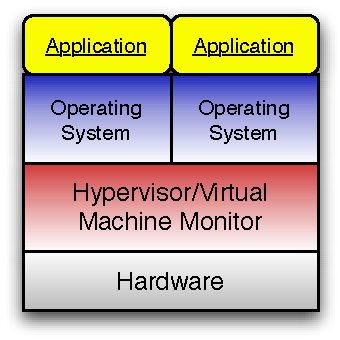
\includegraphics[scale=.75]{architecture-with-virtualization}
    \end{center}
    \caption[Virtualization   architecture]{The   so-called   bare-metal
      virtualization:   A  virtual   machine  monitor   runs   as  small
      ``operating system'' on the  real hardware and provides access for
      virtual machines.}
    \label{fig:arch-virt}
  \end{minipage}
  \end{center}
\end{figure}

This  kind   of  virtualization  is  called   ``full''  or  ``bare-metal''
virtualization  ---  an operating  system  running  in  a virtual  machine
provided by the  VMM thinks it runs on real  hardware. An abstract picture
of such an architecture is shown in Fig.~\ref{fig:arch-virt}.

%%
%% TODO: to be continued
%%

The  virtual machines
(VMs)  ran as  an instance  on the  real hardware  and provided  a logical
machine to  each user. 

Later  on with  the emergence  and  broad availability  of cheap  Personal
Computers  the demand  for virtualization  shrank. But  with the  birth of
dozens of  operating and hardware systems (DOS,  Windows, Linux, Free-BSD,
Mac OS and many more),  the need for virtualization technologies came back
into mind  and today's computers are  powerful enough to  provide VMs. The
main scenario in that case is, that software developers want to be able to
test their applications on many  of these systems without having access to
a physical system.

\subsection{Taxonomy}

There are several software  and hardware solutions available which provide
such a  virtualized platform.  One can distinguish  these attempts  by the
following criteria (see \cite{virtualization-survey}):

\begin{description}
\item[Emulation] An  emulator simulates the complete hardware  and as such
  allows the execution of unmodified guest operating systems. Examples are
  Bochs and Qemu (without its acceleration techniques) for instance.
\item[Native vir\-tu\-ali\-za\-tion] The  virtual machine in this approach
  simulates  enough hardware  to let  an unmodified  guest to  be  run. As
  mentioned earlier, this field was  pioneered within the 1960s with CP-40
  and  CP[-67]/CMS (all  predecessors of  IBMs VM).   Examples  are VMware
  Workstation, VMWare Server, z/VM etc..
\item[Paravirtualization]  In  this case,  the  virtual  machine does  not
  necessarily need to simulate hardware, instead it provides a special API
  to which a guest system has to  be ported. That means one can not run an
  unmodified guest on top of a paravirtualized machine --- modern hardware
  virtualization  techniques  such  as  Intel's  Vanderpool  VT  or  AMD's
  Pacifica make this possible, too. Examples in this field include Xen and
  VMWare ESX Server.
\item[Operating system-level  virtualization] This kind  of virtualization
  uses the same  kernel for the host and all guest  systems --- the guests
  run  ``within''  the  host.   Examples include  Solaris  Containers  and
  Free-BSD Jails.
\item[Application  virtualization] The  Java virtual  machine is  a widely
  known  and used implementation  of this  technique. Programs  written in
  Java are compiled into ``Java byte  code'' which is then executed by the
  Java   runtime   environment   (virtual   machine  plus   an   operating
  environment).  This  approach made it  possible to create  software that
  can  be run  on every  platform for  which a  port of  the  Java virtual
  machine exists.
\end{description}

In this  work I am  dealing with the ``paravirtualization''  technique and
especially with the Xen.

\subsection{Xen --- what's that again?}

Xen  \cite{xen}  is  a  virtualization  technology to  partition  a  given
physical machine into smaller virtual  machines (i.e. VMs).  Each of these
VMs have  their own main memory,  file space and most  important their own
operating system.  Xen belongs  to the paravirtualization group of virtual
machines  and  thus  provides  a  small virtualization  layer  called  the
\emph{hypervisor} or  \emph{Xen Virtual Machine  Monitor}. This hypervisor
provides an API to which a guest operating system must be ported.


\begin{figure}[htbp]
  \begin{center}
    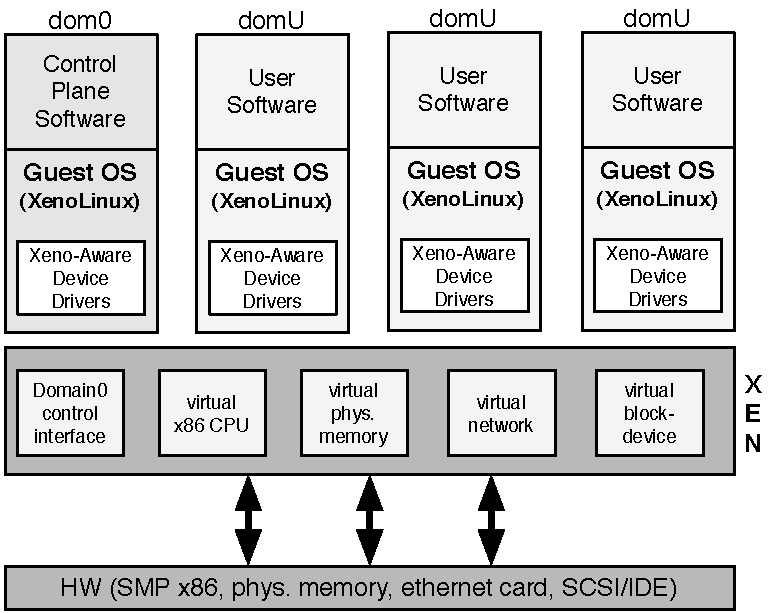
\includegraphics[height=8cm]{xen-architecture}
  \end{center}
  \caption[Xen architecture]{The structure of a system running the Xen
    hypervisor and several user domains (taken from \cite{xen-art})}
  \label{fig:xen-architecture}
\end{figure}

Xen  virtual  machines  (see Fig.~\ref{fig:xen-architecture})  are  called
``domains''  and   the  top-level  or   most  privileged  one   is  called
\texttt{Domain-0} or \texttt{dom0}\footnote{dom-zero} --- this is the only
one, that  is able  to create new  virtual machines.  The  virtual machine
instances  beside  \texttt{dom0} are  called  ``user  domains'' or  called
\texttt{domU}s, they are less privileged  and do not have direct access to
the (real) hardware.

The  operating  system running  within  a  \texttt{domU} accesses  virtual
hardware  provided by  the Xen-architecture  (SCSI or  IDE  controllers to
access  virtual  hard  drives,  network  interface cards  to  be  able  to
communicate with other computers and so on).

\subsection{Nomenclature}

The area of  virtualization needs a small vocabulary, which  I am going to
introduce in this section.  I am only considering Xen as relevant for this
thesis, so I am concentrating especially on vocabulary found in that area.
\begin{description}
\item[image] An image  is a file that contains  a complete file-system and
  can  be  ``mounted'' by  an  operating  system as  if  it  was a  normal
  file-system on  a physical drive.  On  such an image could  be all files
  that are  needed to run  an operating system  for instance or  a special
  application installation.
\item[node] A machine  or a node is in this work  considered as a computer
  that  can be accessed  through Internet  technology, i.e.  it has  an IP
  address and thus speaks TCP.
\item[task] A  task or an application is  a piece of software  that a user
  desires to execute.
\item[URI]   A   URI  is   a   ``Universal   Resource  Identifier''   (see
  \cite{rfc2396}).
\end{description}

\section{Execution environment}

I have already mentioned, that the approach taken in this work is based on
``separation  through  virtualization''.   This  section  deals  with  the
requirements to  the system  and what a  user should  be able to  do.

An \emph{execution environment} should at least meet the following points:
\begin{enumerate}
\item start new tasks
\item stop running tasks
\item list running tasks
\item query the status of tasks
\item reservation of remote resources
\item providing input data for a task
\item retrieving generated data from a finished task
\end{enumerate}

Additionally this work is  about a \emph{Xen based} execution environment,
so that  means that if a user  wants to execute an  application the system
will create a new virtual machine.

The application  need not to  be run  locally, it can  be run on  a remote
system  --- the  only requirement  is, that  the data  can  be transferred
there.  That will be the base functionality of the here designed system:

\begin{quote}
  \emph{``executing applications on remote systems using Xen instances''}
\end{quote}

\paragraph{Starting an application}

To be able to create a virtual  machine on the remote site the user has to
specify not only  the application she wants to run but  also an image that
contains the  required operating  system.  The execution  environment then
takes care of starting up the  virtual machine with the provided image and
eventually execute the application.

For later  reference to the  just created task, the  execution environment
must assign a unique identifier that can  be used by the user to manage or
query the status of that task.

\paragraph{Managing running tasks}

Given  that the user  started a  task earlier,  he may  want to  query the
status of  that task. He could  also want to abort  the task, if  he is no
longer  interested in  it. The  execution  environment gave  out a  unique
identifier with which the user now can refer to the task.

The may also be interested in an overview of tasks that he has started, so
the environment  should present  him a  list of all  his tasks  along with
their states.

\paragraph{Reserving resources}

A more  advanced usage  is the reservation  of resources in  advance. That
means a user can specify everything she  would as if she wanted to start a
new task but additionally she says  for example when the task shall start. 
The execution environments is required to meet that constraint.

\paragraph{Accessing the data}

Computational programs usually work on some input data and generate output
data of differing  amount. The system I am going to  design must offer the
user functionalities  to transfer  input data to  the virtual  machine and
output data back.

\bigskip

We have now sketched the requirements  to the environment and can now have
a look at its building blocks.

\section{Architecture}
\label{sec:architecture}

This  section  introduces  the  desired architecture  of  the  ``Xen-based
execution     environment''.      The     system    as     depicted     in
Fig.~\ref{fig:architecture}   essentially   consists   of  the   following
components:
\begin{enumerate}
  
\item some kind of a user --- that could be a real person using the system
  on  one hand  or  a script  or some  other  program such  as a  ``Calana
  Broker''        (described        in        \cite{dalheimer05agentbased,
    dalheimer06calanaprotocol}) on the other hand.
  
\item a central  managing daemon running on a Xen  \cite{xen} host or more
  concretely within \texttt{dom0}.  This part is, for instance, accessible
  through a command line, a web service or some other interface. A user in
  general  does  only   talk  directly  to  this  part   of  the  system.  
  Fig.~\ref{fig:architecture} shows this part  as the ``Xen Manager''.
  
\item the third component resides  directly on a Xen instance and provides
  several functions to the  managing daemon (``Xen instance controller''). 
  Functionalities  of this component  include: monitoring  and controlling
  the user's  application, mounting external data  locations and providing
  access to generated results.

\end{enumerate}

\begin{figure}[htbp]
  \begin{center}
%    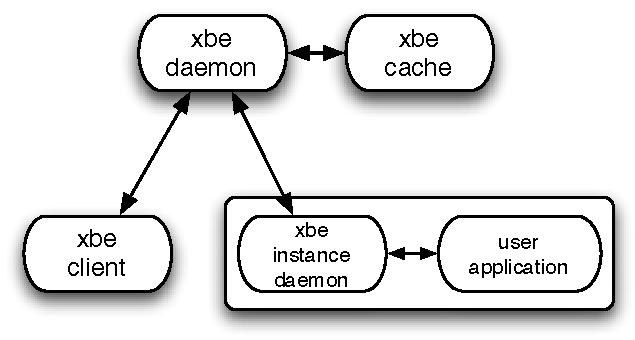
\includegraphics[height=80mm]{architecture-overview}
  \end{center}
  \caption[Architecture overview]{An overview over the conceptual
    architecture}
  \label{fig:architecture}
\end{figure}

The other parts of the figure are storage locations, such as ``image'' and
``data'' locations.   That are those sites  where a user  can store images
with applications  or data  and that  can be accessed  by the  system.

The  application images  for  instance  must be  accessible  by the  ``Xen
Manager'' to be able to boot  up a virtual machine.  Data images, used for
input to  and output from the  application, must be made  available to the
``Xen  instance  controller''.  The  ``image  cache''  can  be seen  as  a
secondary image  location, it can be  used to store images  to access them
faster (``locality of reference'', \cite{locality-principle}).

The next  section deals with  several use cases  that are of  interest for
users and administrators of this system.

\section{Use cases}

In  an  earlier   section  I  have  shortly  described,   what  the  basic
requirements to this  system are and now  I am going to show  you some use
cases and which parts of the architecture are involved in each.

The  big  picture  is  shown  in  \ref{fig:system-usecases},  it  shows  a
compendium of several possible use cases from a very high level.

\begin{figure}[htbp]
  \begin{center}
%    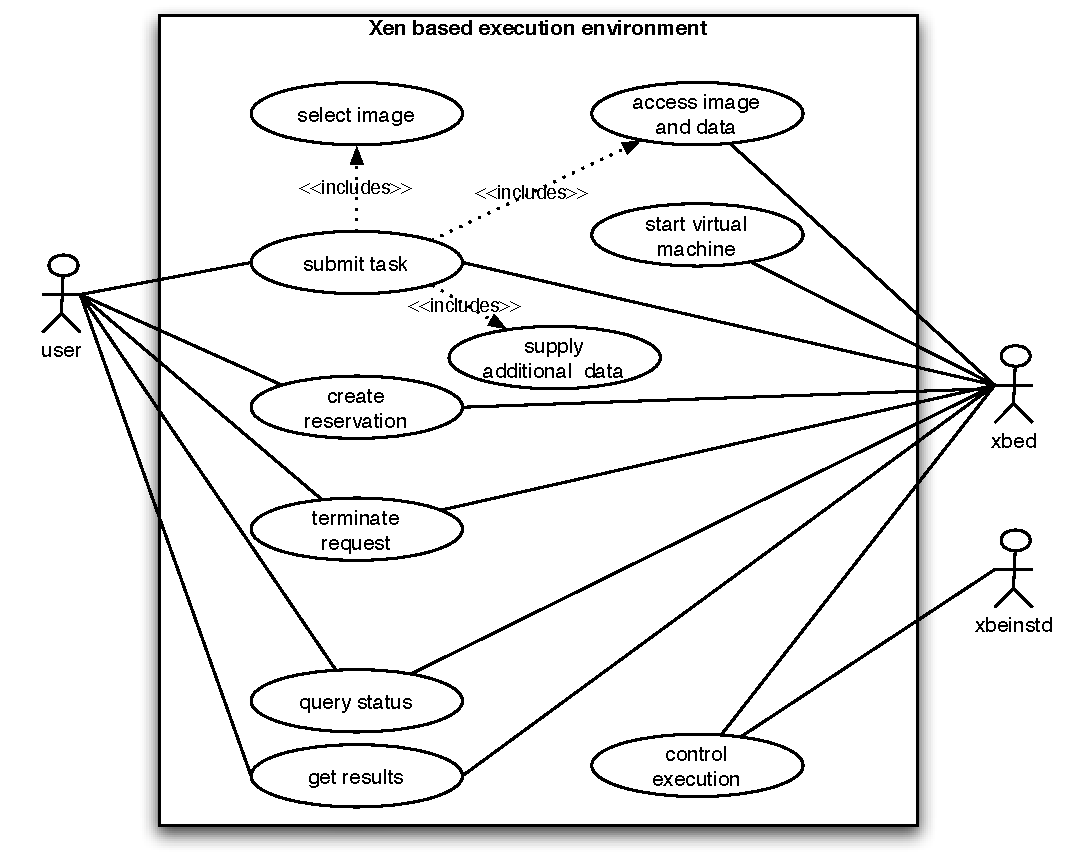
\includegraphics[width=0.9\textwidth]{system-usecase}
  \end{center}
  \caption[Use case overview]{an overview over several possible use cases}
  \label{fig:system-usecases}
\end{figure}

The use cases are split into several scenarios which can arise during that
particular  case. Now  let's go  through each  use case  step by  step and
analyze on that way where possible problems could occur.

\subsection{Use case 1: image submission}
\label{uc:1}

The  first use case  is about  the submission  of images,  that are  to be
executed on a remote host. The main  objective of this use case is how the
user can specify which image he wants to submit and eventually be run.

\subsubsection{Scenario 1.1 --- submitting a single image}

The easiest scenario  is in which the user only has  one image. This image
contains  everything: the  operating  system, the  application and  needed
input  data.  That  means  all needed  information  is within  the image.  
Figure~\ref{fig:arch-uc-1.1} shows the  relevant parts of the architecture
that are involved in this scenario.

\begin{figure}[htbp]
  \begin{center}
%    \includegraphics[height=8cm]{architecture-uc-1-1}
  \end{center}
  \caption[Architecture UC 1.1]{parts of the architecture relevant to use
    case 1.1}
  \label{fig:arch-uc-1.1}
\end{figure}

The user specifies the location (i.e. an URI) of the image and passes this
information to  the ``Xen Manager'' along  with a description  of the task
that  he desires  to execute.  The ``Xen  Manager'' will  then  attempt to
download the  image from the  specified location. 

\begin{figure}[htbp]
  \begin{center}
%    \includegraphics[height=8cm]{sequence-image-submission-1}
  \end{center}
  \caption[Sequence UC 1.1]{sequence diagram for the image submission}
  \label{fig:seq-uc-1.1}
\end{figure}

When the image  has been successfully retrieved, the  ``Xen Manager'' will
create  a  special  Xen  instance  to  run the  image.

\bigskip

\paragraph*{When will the image be started?}

The answer simply  is ``it depends''. That is because  the boot up process
takes some  time and may vary  of course.  Additionally the  image must be
transferred from some  location to the server and  that consumes even more
time. If a user wants to have some guaranty, it will be required, that
\begin{enumerate}
\item the image does already reside on the server
\item a reservation has been made
\end{enumerate}

This  particular topic is  a use  case on  its own  and will  be discussed
later.

\paragraph*{What happens if errors occur?}

Errors can occur  in each step of the  submission.  During the interactive
part (i.e. submission  of the job description) errors  may be communicated
directly back to the user.

If an error  occurs during the transfer of some image,  there is no direct
way  to tell  the user  about it.   But  the user  can check  later on  if
something went  wrong using the  unique identifier she  got.  Additionally
could there be  a notification service, to which  the user subscribes with
the unique identifier. This service could then send out messages to inform
the user.

\subsubsection{Scenario 1.2 --- submitting several images}

In the first  scenario all data had to be within  one image, this drawback
is addressed in this scenario. The components used in this scenario are
shown in Fig.~\ref{fig:arch-uc-1.2}

Along with an  image the user can specify locations  from which input data
may be retrieved  and to which generated data should  be sent --- commonly
known as staging operations. These locations can be any URI as long as the
appropriate operation (read/write) can be executed.

\begin{figure}[htbp]
  \begin{center}
%    \includegraphics[height=8cm]{architecture-uc-1-2}
  \end{center}
  \caption[Architecture UC 1.2]{parts of the architecture relevant to use
    case 1.2}
  \label{fig:arch-uc-1.2}
\end{figure}

\subsection{Use case 2: caching of images}
\label{uc:2}

Imagine a user,  who wants to execute the same  application several times. 
That would  mean he has  to submit the  same image again and  again, which
imposes a heavy load on the network connecting user and provider (i.e. the
host  on which the  Xen Manager  runs). It  is wise  to provide  a caching
mechanism, that allows the user to store his image at server-side.

The    architecture    needed    for     this    case    is    shown    in
Fig.~\ref{fig:arch-uc-caching}.

\begin{figure}[htbp]
  \begin{center}
%    \includegraphics[height=5cm]{architecture-uc-caching-1}
  \end{center}
  \caption[Architecture UC 2]{parts of the architecture relevant for caching}
  \label{fig:arch-uc-caching}
\end{figure}

\paragraph{How gets the image transferred?} There are two answers to this
question, that can be  categorized into ``active'' and ``passive'' caching
from the user's point of view.
\begin{itemize}
\item Prior to any job submission, the user (actively) transfers the image
  to the server  (Fig.~\ref{fig:seq-image-caching-1}).
  \begin{figure}[htbp]
    \begin{center}
%      \includegraphics[width=0.75\textwidth]{sequence-image-caching-1}
    \end{center}
    \caption[Image caching sequence 1]{actively caching an image}
    \label{fig:seq-image-caching-1}
  \end{figure}
  Later  on, when the  user wants  to submit  a job,  he passes  the cache
  location --- represented by a unique identifier --- to the server.
  
\item The user specifies a job description as described in use case 1. The
  Xen Manager  not only  retrieves the  image to start  the job,  but also
  stores it in the cache (Fig.~\ref{fig:seq-image-caching-2}).
  \begin{figure}[htbp]
    \begin{center}
%      \includegraphics[width=0.75\textwidth]{sequence-image-caching-2}
    \end{center}
    \caption[Image caching sequence 2]{an image gets passively cached by
      the Xen Manager}
    \label{fig:seq-image-caching-2}
  \end{figure}
\end{itemize}


\paragraph{How is the cached image referenced?} To efficiently use cached
images, it is required that the user can reference them somehow. More than
one solution is here possible, too.
\begin{itemize}
\item The user uses the unique  identifier he got when he stored the image
  in   the    cache   in   the    first   place,   this   is    shown   in
  Fig.~\ref{fig:seq-image-caching-3}.
  \begin{figure}[htbp]
    \begin{center}
%      \includegraphics[width=0.75\textwidth]{sequence-image-caching-3}
    \end{center}
    \caption[Image referencing]{retrieving a referenced image from the cache}
    \label{fig:seq-image-caching-3}
  \end{figure}
\item The user  queries the Xen Manager to give him  a descriptive list of
  all   cached   images,   that   are   accessible  by   the   user   (see
  Fig.~\ref{fig:seq-image-caching-4}).   Descriptive means here,  that the
  user is presented with some detailed information about the images.
  \begin{figure}[htbp]
    \begin{center}
%      \includegraphics[width=0.75\textwidth]{sequence-image-caching-4}
    \end{center}
    \caption[Image referencing]{retrieving a referenced image from the cache}
    \label{fig:seq-image-caching-4}
  \end{figure}
\end{itemize}

The    components   involved    in    this   scenario    are   shown    in
Fig.~\ref{fig:arch-referencing-images-1}.
\begin{figure}[htbp]
  \begin{center}
%    \includegraphics[height=5cm]{architecture-referencing-cached-images-1}
  \end{center}
  \caption{Architecture of use case 2}
  \label{fig:arch-referencing-images-1}
\end{figure}


\subsection{Use case 3: image deployment}

This use case  deals with the starting process of  images. The Xen Manager
uses the image  that the user specified and starts up  a Xen instance. The
steps  required   to  start   up  such  a   new  instance  are   shown  in
Fig.~\ref{fig:seq-image-deployment-1} and consist of:
\begin{enumerate}
\item  The instance  itself has  to be  started.
\item  During  that an  instance  controller  is  being started  ---  this
  controller  is   responsible  for  starting,   monitoring  and  stopping
  applications and several other housekeeping functionalities.
\item The Xen Manager connects to the instance controller, thus confirming
  that the instance is fully available.
\end{enumerate}

\begin{figure}[htbp]
  \begin{center}
%    \includegraphics[height=5cm]{sequence-image-deployment-1}
  \end{center}
  \caption[Image deployment sequence]{the steps required to be taken to
    start up a new instance}
  \label{fig:seq-image-deployment-1}
\end{figure}

After  successfully  connecting  from  the  Xen Manager  to  the  instance
controller, both  sides are in  the state ``instance  controllable'', that
means that:
\begin{itemize}
\item applications can be started through the controller
\item started applications can be monitored and controlled
\end{itemize}

Additionally  it   is  possible  to   retrieve  the  streams   of  started
applications.        The        architecture       as       shown       in
Fig.~\ref{fig:arch-deployment-1}   is  now   enriched   by  the   instance
controller running on a Xen instance.

\begin{figure}[htbp]
  \begin{center}
%    \includegraphics[height=5cm]{architecture-deployment-1}
  \end{center}
  \caption[Image deployment architecture]{a Xen Manager controlling three
    Xen instances}
  \label{fig:arch-deployment-1}
\end{figure}


\subsection{Use case 4: controlling and monitoring}

A  full-fledged execution  environment demands  mechanisms to  control and
monitor its activities.   At all times the user must be  able to:
\begin{itemize}
\item  query the status  of her  running application  --- the  sequence of
  actions is shown in Fig.~\ref{fig:seq-status-query-1}.
  \begin{figure}[htbp]
    \begin{center}
%      \includegraphics[height=5cm]{sequence-status-query-1}
    \end{center}
    \caption[Querying the status]{a user querying the status of his application}
    \label{fig:seq-status-query-1}
  \end{figure}
\item and  she should also be able  to abort the very  same execution (see
  Fig.~\ref{fig:seq-abort-task-1}).
  \begin{figure}[htbp]
    \begin{center}
%      \includegraphics[height=5cm]{sequence-abort-task-1}
    \end{center}
    \caption[Aborting a running task]{a user requesting the abortion of a
      running task}
    \label{fig:seq-abort-task-1}
  \end{figure}
\end{itemize}

The OGSA-BES  draft \cite{ogsa-bes} defines a  standardized description of
job states (Fig.~\ref{fig:ogsa-bes-model-1})  which can easily be extended
without breaking  components relying on the  ``non-extended'' model.  This
standard  can be used  to describe  the states  of an  application running
within a Xen instance.

\begin{figure}[htbp]
  \begin{center}
%    \includegraphics[height=5cm]{ogsa-bes-state-model-1}
  \end{center}
  \caption{The basic OGSA-BES state model}
  \label{fig:ogsa-bes-model-1}
\end{figure}


\paragraph{What, if the application is not running yet?}

Imagine a  user requesting the current  state of his  newly submitted job,
the Xen  Manager answers all  questions as best  as it can. That  means he
would       for       example       react      as       described       in
Table~\ref{tab:monitor-cases-overview}.
\begin{table}[htbp]
  \begin{center}
    \begin{tabular*}{0.9\textwidth}{p{0.4\textwidth}|p{0.4\textwidth}}
      current situation & state returned \\ \hline\hline
      image not yet available & \texttt{pending} (image loading)\\ \hline
      instance not yet started & \texttt{pending} (instance) \\ \hline
      application not yet started & \texttt{pending} (application) \\ \hline
      image could not be retrieved & \texttt{failed} (image retrieval) \\ \hline
      instance could not be started & \texttt{failed} (instance) \\ \hline
      application could not be started & \texttt{failed} (application)
    \end{tabular*}
    \caption[States returned by the Xen Manager]{States returned by the Xen Manager in several cases}
    \label{tab:monitor-cases-overview}
  \end{center}
\end{table}


\subsection{Use case 5: resource reservation}

An advanced subject is to provide advance reservation. That means that the
user  has the  possibility  to tell  the  Xen Manager,  that  he needs  an
instance for a given  time and at a specific point in  time.  Later on the
user can specify which image the Xen Manager should use.

The steps taken are presumably as follows:
\begin{enumerate}
\item The user  makes a reservation of some resource,  i.e. number of CPUs
  for a given duration --- five hours  for example --- and a point in time
  at       which      the       reservation      may       start      (see
  Fig.~\ref{fig:seq-advance-reservation-1}).
  \begin{figure}[htbp]
    \begin{center}
%      \includegraphics[width=0.75\textwidth]{sequence-advance-reservation-1}
    \end{center}
    \caption{Making a reservation}
    \label{fig:seq-advance-reservation-1}
  \end{figure}
  
\item After obtaining  a (unique) reservation ID, the  user can submit any
  job  he  likes  and  he  is  guaranteed, that  job  will  start  by  the
  reservation's start time.
  \begin{figure}[htbp]
    \begin{center}
%      \includegraphics[width=0.75\textwidth]{sequence-advance-reservation-2}
    \end{center}
    \caption{Submitting a job using a reservation}
    \label{fig:seq-advance-reservation-2}
  \end{figure}
  
\item The  Xen Manager acts as if  it was an ordinary  job submission, but
  this time he waits with starting up the instance until the start time of
  the reservation is reached.
  \begin{figure}[htbp]
    \begin{center}
%      \includegraphics[width=0.75\textwidth]{sequence-advance-reservation-3}
    \end{center}
    \caption{Starting an instance with a reservation}
    \label{fig:seq-advance-reservation-3}
  \end{figure}
\end{enumerate}

So  the  actual submission  of  an  image is  split  into  two parts,  the
reservation  part  and  the  eventual  assignment  of  an  image  to  that
reservation.

It seems  to be  very simple but  there are  some problems that  come into
mind.

\paragraph{What happens if the image is not available?}

This case can easily been run into, if the reservation shall start but the
image is not yet available. The user has to be informed about that and the
job can not be run.

One  solution  to  that  is   to  provide  the  image  before  making  any
reservations or  submissions using that  image, thus the user  makes sure,
that  the image  will be  available when  needed. Another  (less failsafe)
solution  is to  have  enough time  between  submission and  start of  the
reservation  ---  this  highly  depends  on  how fast  the  image  can  be
retrieved.

\paragraph{What if a reservation ends before the application exits}

This may  happen, since  users can not  always exactly foresee  when their
application will  end and thus  may specify a  too short duration  for the
reservation.  Ordinary batch-scheduler usually  give a little more time to
the application and stop it (i.e.  forcing it to quit) eventually.

\begin{figure}[htbp]
  \begin{center}
%    \includegraphics[width=0.75\textwidth]{sequence-advance-reservation-4}
  \end{center}
  \caption{Suspending an instance}
  \label{fig:seq-advance-reservation-4}
\end{figure}

Xen provides  the possibility  to suspend the  instance and  continuing it
later  (Fig.~\ref{fig:seq-advance-reservation-4}).  The  problems involved
with suspension of  a running instance are discussed in  the next use case
``check-pointing''.


\subsection{Use case 6: check-pointing}

In Fig.~\ref{fig:seq-advance-reservation-4} you  have seen how an instance
has been  suspended in the case  of reservation expiry  --- suspension can
also    be    used    to    provide    the   user    with    a    snapshot
(\cite{distributed-snapshots}) or check-pointing mechanism.

The steps taken  are essentially the same ---  suspending the instance due
to some event,  saving the state and resuming it later  --- this is called
an ``offline snapshot''.

\paragraph{What are the events?}

As        in         use        case        ``advance        reservation''
(Fig.~\ref{fig:seq-advance-reservation-4}),   one   event   may   be   the
expiration of a reservation, but there are more:

\begin{itemize}
\item the application itself triggers  an event, indicating that now would
  be a good point to do a snapshot
\item a snapshot is taken regularly by the system
\item  the user  wants to  make a  snapshot (manually  triggered)  --- for
  instance after four hours of computation.
\end{itemize}


\paragraph{Problems that can occur}

One big  problem of taking a  snapshot in this way  are active connections
(e.g.  TCP  connections) from the instance,  those cannot be  saved by the
system  and  must  therefore  be  reinitialized by  the  application  upon
resuming.

The application  does not necessarily need  to know that  the instance has
been suspended, so it  seems to it like a link or  network failure. As you
can  see, the  application  must be  able  to recover  from  that kind  of
failure.

Even worse are connections{\bf to}  the instance, since after resuming the
IP address  of the instance  may have changed.  To overcome this,  the Xen
Manager is required to assign the same address to this instance.

\subsection{Use case 7: updating existing images}

So far,  we were only interested  in how a  user is involved in  the image
execution  process.  But  what  about  an site  administrator  who has  to
administer all the cached or especially provided application images. Those
applications and  operating system distributes  need updates from  time to
time, but there could be plenty of such images residing in the database.

This problem  directly leads to  the need for  an automated task  that can
update the software components within  an image and execute a special test
case designed to confirm that everything is still working.

%%% Local Variables: 
%%% TeX-master: "main.tex"
%%% End:

\setchapterpreamble[o]{%
  \dictum[Lao-tzu]{\textit{``A journey of a thousand miles begins with
      a single step.''}}}

\chapter{Fundamentals}
\label{cha:fundamentals}

This chapter  describes some basic principles,  that are going  to be used
throughout this thesis. For example, the \emph{Extensible Markup Language}
is used  for all  messages, that  are sent between  the components  of the
execution  environment. A special  description language,  called \emph{Job
  Description Language}, will  be used for the submission  of tasks to the
system.   The  tasks' states  are  represented  using  the extensible  job
state-model definition of the \emph{Basic Execution Service}.

The  Calana Grid-scheduling  approach will  be shortly  discussed  in this
chapter, too.  The here proposed  execution environment is supposed  to be
used as a possible back-end resource of the Calana system.

The  final parts  of this  chapter  consider message  security. At  first,
public-key  cryptography will  be  discussed and  then  two available  and
widely used  technologies for  securing communication between  two parties
are discussed. These two  technologies are \emph{Transport Layer Security}
and \emph{Message Layer Security}.

\section[The Extensible Markup Language]
{The Extensible Markup Language (\gls{glo:XML})}
\label{sec:fundamentals:xml}

The Extensible Markup Language \cite{xml}  is a simple, yet very flexible,
plain text based description format. The format represents a subset of the
\emph{Standard  Generalized Markup Language}  (SGML).  It  can be  used in
variety of ways and even more usages are discovered still. Examples of XML
can be found in  \emph{XHTML}, \emph{RSS}, \emph{Atom}, \emph{Math-ML} and
many more.   Due to the  structured semantics of  XML, more and  more file
formats are  nowadays based  on XML,  thus replacing the  old INI  or Unix
\texttt{rc}  files  --- a  very  popular exemplar  in  this  field is  the
\emph{OASIS Open Document Format for Office Applications}.

An XML-file is  an ordinary plain text file, that  could have been created
by any text  editor.  The most important building  blocks of XML-files are
\emph{elements}, \emph{attributes} and \emph{text}.

Elements   are  \emph{logical  structures},   that  can   have  additional
attributes and  sub-elements or \emph{children}, whereas  the children can
either be other elements or text.  The following example shows you a small
XML document. Every XML  document contains \textbf{exactly one} designated
\emph{root} element, which is simply the first element in the document.

For parsing purposes,  an XML document can be represented  as a tree, this
is  shown in Figure~\ref{fig:xml-example}.   A widely  used model  for the
in-memory  representation of  XML documents  is the  \emph{Document Object
  Model} (DOM).  Most  of the available XML parsers,  provide an interface
for parsing a document into  an in-memory representation that follows this
model. The programmer  can then simply add, delete  or modify elements and
attributes by  using an object-oriented  interface.  Using the  example in
Figure~\ref{fig:xml-example}, a programmer could for instance iterate over
all children  of the \texttt{root}-element, that have  a tagname (\ie the
name  of the  element) equal  to ``child''  --- in  this case,  that would
result in just two elements.

\begin{figure}[h]
  \centering
  \begin{tabular}{rc}
    \begin{minipage}[c]{.35\textwidth}
      \begin{lstlisting}[language=XML]
<root foo="bar">
  <child/>
  Some text
  <child>More text</child>
</root>
      \end{lstlisting}%
    \end{minipage} &
    \begin{minipage}[c]{.35\textwidth}
      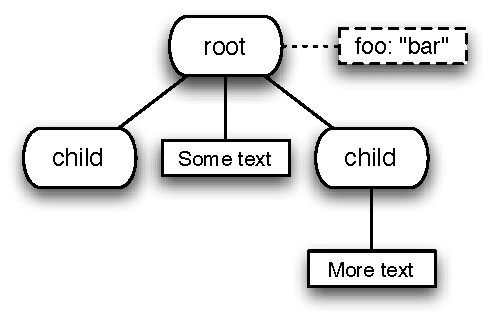
\includegraphics[width=5cm]{xml-example}
    \end{minipage}
  \end{tabular}
  \caption{A simple XML example}
  \label{fig:xml-example}
\end{figure}

\subsection{Namespaces}

XML  documents   may  contain  elements  and   attributes  from  different
vocabularies (\ie different document  types). To resolve ambiguity between
the  involved   vocabularies,  the  W3C  recommends  the   use  of  unique
\emph{Namespaces}  that are  assigned  to each  element.   A document  may
contain a  \emph{default}-namespace to which  all elements belong  that do
not  have  a  special  namespace  assigned.   Within  a  single  document,
namespaces are given  a logical name. The logical  name itself is assigned
the unique Namespace identifier (\eg a \gls{glo:URI}). Some namespaces and
common   ``names''   for  them   are   given   in   the  following   table
(Table~\ref{tab:namespaces}):

\medskip

\begin{table}[h]
  \centering
  \begin{tabular}{@{}ll@{}}\toprule
    logical name        & \multicolumn{1}{l}{namespace URI} \\ \midrule % header
    \texttt{xsd}        & \url{http://www.w3.org/2001/XMLSchema} \\
    \texttt{jsdl}       & \url{http://schemas.ggf.org/jsdl/2005/11/jsdl} \\
    \texttt{jsdl-posix} &  \url{http://schemas.ggf.org/jsdl/2005/11/jsdl-posix} \\
    \texttt{dsig}       & \url{http://www.w3.org/2000/09/xmldsig#} \\
    \texttt{bes}        & \url{http://schemas.ggf.org/bes/2006/08/bes-activity} \\
    \texttt{xbe}        & \url{http://xenbee.berlios.de/schemas/xbe/2007/01/xbe} \\
    \texttt{xsdl}       & \url{http://xenbee.berlios.de/schemas/xsdl/2007/01/xsdl} \\
    \bottomrule
  \end{tabular}
  \caption[XML Namespaces used in this work]{Important namespaces}
  \label{tab:namespaces}
\end{table}

Namespaces  are   specified  in  the  XML  using   the  special  attribute
\texttt{xmlns}.     An   attribute    of   an    element,    which   reads
\texttt{xmlns="www.example.com"}, sets the  default namespace to the given
URI, while  \texttt{xmlns:foo="www.example.com"} makes the  same namespace
known as the logical name  ``foo''. In another document the same namespace
could as well have been assigned the logical name ``bar''.

To specify  that a  given element  belongs to a  namespace other  than the
default namespace, the  element's name is prefixed by  the logical name of
the namespace,  \eg \texttt{foo:child} means, that  the ``child'' element
belongs to the namespace defined by ``foo''.

\subsection{Validation of XML documents}
\label{sec:xml-validation}

A  really nice  and very  useful  addition to  XML is  the possibility  to
\emph{validate}  an XML  document.  There  are two  mechanisms  to provide
validation,    the    \emph{Document    Type   Definition}    (DTD)    and
\emph{XML-Schema}.

\subsubsection{Document Type Definition}

A DTD defines for a particular  document what elements are allowed and how
their attributes look like. The  composition of elements to form container
(\ie parent)   elements  can   be   described  in   a  rudimentary   way.
Unfortunately, the  DTD uses  its own syntax,  that has nothing  in common
with  the syntax of  an XML  document. For  an author  of an  XML document
type\footnote{for example the configuration file format of an application}
that means in particular, that he has to learn two different syntaxes.

\subsubsection{XML-Schema Definition}

XML-Schema is  itself defined  using XML as  its description  language and
obsoletes the  DTD. It is much  more powerful, for instance,  an author is
able  to   restrict  the   actual  data  an   element  or   attribute  may
contain.  Let's for  instance  say, a  given  attribute can  only take  on
non-negative  integers.    To  reflect  this  constraint   in  the  schema
definition,  the   author  would  set   the  type  of  the   attribute  to
\texttt{xsd:nonNegativeInteger}.

There are many predefined data types, an author may use to create new data
type constraints.  An XML-Schema validator complains, if  a document, that
is  supposed to  conform  to  that schema,  contains  the just  introduced
attribute with a negative value, \eg $-1$.

\bigskip

The advantages of XML-Schema over a DTD are obvious.  When using DTDs, the
application  was  responsible to  check  the  validity  of each  used  XML
document  type  itself. That  means,  the  same  functionality had  to  be
implemented over and over again, \ie each time a new application wants to
make use of a given XML document type. While using XML-Schema definitions,
the author of  an XML document type defines  the validity constraints just
once and any application  may rely on that. To make that  clear, here is a
small  example:  Suppose there  is  a  definition  for an  element  called
``\texttt{entry-id}'',  which may  only take  on positive  integer values.
Since a DTD  does not support constraints on  data types, each application
must check  for itself if  the value matches  that type. Now  suppose, the
constraint  for  that  element is  changed,  so  that  the number  $0$  is
included, as  well ---  in each application,  the validation code  must be
modified to match the new constraint.

\section[The Job Submission Description Language]
{The Job Submission Description Language (\gls{glo:JSDL})}
\label{sec:fundamentals:jsdl}

\gls{glo:JSDL} is a very extensible XML-based description language for the
submission  of computational jobs.   With \gls{glo:JSDL}  you are  able to
describe  all requirements  that  a  computational job  may  need for  the
submission to  a remote resource  --- mainly the  \gls{glo:JSDL} addresses
grid resources but it is not limited the latter.

Nearly  every  element of  the  \gls{glo:JSDL}  specification may  contain
arbitrary  many  user-defined  elements  from  other  XML  specifications.
Therefore is the  JSDL fully adoptable to any  upcoming user requirements.
If  the  target  system,  for  instance, requires  a  previously  acquired
reservation ---  represented by an  identification number for  example ---
the  \gls{glo:JSDL} would include  an additional  element which  holds all
information regarding the reservation.  Such extension elements are purely
optional and  systems that are  unaware of a particular  extension element
may just neglect it.

The following section roughly describes the most important components that
are needed to form a useful submission description.

\subsection{``Hello World'' with the JSDL}

A    \gls{glo:JSDL}    document     does    always    start    with    the
\texttt{JobDefinition} element,  which is the top-level  element and holds
all required information about the job.

Let's assume a user wants to execute a small program on a remote resource.
The  program  will  indeed be  very  simple,  it  just prints  the  string
``\texttt{Hello World}'' to the  screen. The execution of this application
on the local computer of our user could be similar to:

\begin{minipage}{0.75\textwidth}
  \begin{lstlisting}[language=ksh]
    $ echo Hello World
    Hello World
    $
  \end{lstlisting}
\end{minipage}

This  excerpt  represents  the   execution  in  a  standard  UNIX  command
shell. Note that the \texttt{echo}  program does nothing more than writing
the parameters passed to it to its \texttt{stdout} stream. Now suppose the
user  desires  to execute  the  same program  on  a  remote resource,  the
\gls{glo:JSDL}  document, he  would  write, will  look  somewhat like  the
document shown in Listing~\ref{lst:jsdl-example}.

\bigskip

\begin{center}
  \begin{minipage}{.75\textwidth}
    \lstinputlisting[captionpos=b,backgroundcolor=\color{listingcolor},frame=lines,numbers=left,numberstyle=\tiny,caption={A
      small ``Hello World''-example written in
      \gls{glo:JSDL}},label={lst:jsdl-example},language=XML]{examples/jsdl-example.jsdl}
  \end{minipage}
\end{center}

Note, that  the shown \gls{glo:JSDL}  document describes exactly  the same
execution  the  user  had  previously  performed  locally.   The  executed
\texttt{echo} program  again writes  its arguments to  its \texttt{stdout}
stream.   Different from the  local execution  is in  this case,  that the
output will  be lost, since the  user did not  specify what is to  be done
with generated output. If the user was interested in the program's output,
he had to specify the redirection of  the output stream to some file and a
staging operation, that transfers the created file to some location he has
access to.

\subsection{Important elements}

A typical \gls{glo:JSDL} document consists  of the following parts --- job
identification,  application description,  resource descriptions  and data
staging elements. Only the first two of them have been used in the example
shown in Listing~\ref{lst:jsdl-example} to keep the example simple.

\subsubsection{Job identification}

The \texttt{JobIdentification}  element is used to  hold information about
the job, such as a descriptive  name, that is mostly interesting for human
beings.  Nonetheless it  may hold additional information that  could be of
interest to  applications processing the document ---  such as annotations
(\eg a  unique task  identification number  could  be stored  in such  an
annotation).

\subsubsection{Application}

With the \texttt{Application} element, a user describes the program itself
---  \ie the  real executable,  that  is going  to  be  used.  A  special
extension --- \texttt{POSIXApplication}, also defined in the specification
\cite{jsdl-spec}   ---   can  be   used   to   describe  executables   for
\gls{glo:POSIX}-compliant   operating  systems  \cite{posix}.    You  have
already      seen     the     usage      of     this      extension     in
Listing~\ref{lst:jsdl-example},  where it  had  been used  to specify  the
execution of the \texttt{echo} command line program.

\subsubsection{Resources}

This element can be used  to describe various resource requirements of the
application. Some of the many resource types one can use are listed below.

\begin{itemize}
\item the number of CPUs the job requires
\item the operating system required by the job
\item amount of virtual memory that must be available for the job
\item file-systems  and their expected  mount-points
\end{itemize}

All  specified file-systems  must  be  made available  for  the job  prior
execution. Every file-system specification  defines a unique name that can
be used to refer to that particular file-system in other elements, such as
staging operations.  Thereby the  user can define \emph{logical names} for
special directories within the execution environment of the task.
  
\subsubsection{Staging operations}

The   \texttt{DataStaging}    element   is   used    to   define   staging
operations.  These operations  can either  be  \emph{Stage-In} operations,
which  refer  to files  that  have to  be  transfered  into the  execution
environment  prior   the  execution  of  the   task,  or  \emph{Stage-Out}
operations, which refer  to transfers that have to be  made after the task
has been executed.

A user may  specify the \texttt{DataStaging} element as  often as he likes
to.   The most  relevant elements  within  a staging  instruction are  the
\texttt{Source}  and \texttt{Target}  elements, both  of them  can  hold a
\texttt{URI}  element  to  specify  a  generic  location.   The  mandatory
\texttt{FileName} element points to  an actual file within the file-system
hierarchy of the execution environment of the task. The actual location of
a file can be given relative  to a previously defined file-system, in this
case the \texttt{FilesystemName} element must be specified and is required
to contain the logical name of \texttt{FileSystem} resource.

\bigskip

As  you can  see,  the  \gls{glo:JSDL} is  a  really powerful  description
language and  it covers many,  if not all,  of the requirements  a typical
computational job  may have. And if it  does not cover a  special topic on
its own,  one is able  to extend the  elements of the  \gls{glo:JSDL} with
user-defined elements.

\section[The Basic Execution Service]{The Basic Execution Service (BES)}
\label{sec:fundamentals:bes}

The \emph{Basic Execution Service} \cite{ogsa-bes} is a specification that
defines  a service (\eg a  web service)  which provides  functionality to
control \emph{Activities}.   A user is able  to submit an  activity to the
execution service and  can later on control and  monitor that activity ---
using web service calls, for instance.

Control  of  the  activity  is   basically  limited  to  a  request  which
\emph{terminates} the  activity. The monitoring of an  activity results in
returning the activity's current state.

The state  of an activity is  modeled using a finite  state automaton. The
specification of the \gls{glo:BES}  incorporates a rather simple, but very
extensible, state  machine for  activities. It comprises  a total  of just
five  states  an  activity  can  be  in  at  any  time:  \texttt{Pending},
\texttt{Running},       \texttt{Finished},       \texttt{Failed}       and
\texttt{Terminated}.

States of the \gls{glo:BES} are represented using a XML specification. The
element  which  represents the  current  state  of  an activity  is  named
\texttt{ActivityStatus} and belongs to  the \emph{bes} namespace as it has
been  defined  in Table~\ref{tab:namespaces},  the  state  itself is  then
specified using the \texttt{state} attribute:

\begin{lstlisting}[language=XML]
  <bes:ActivityStatus state="Running"/>
\end{lstlisting}

The     state     machine,     or     state-model,     is     shown     in
Figure~\ref{fig:bes-basic}. To  reflect the request for  termination of an
activity,  each state,  except the  final  states of  course, provides  an
outgoing transition to the \texttt{Terminated} state.

\begin{figure}[h]
  \centering
  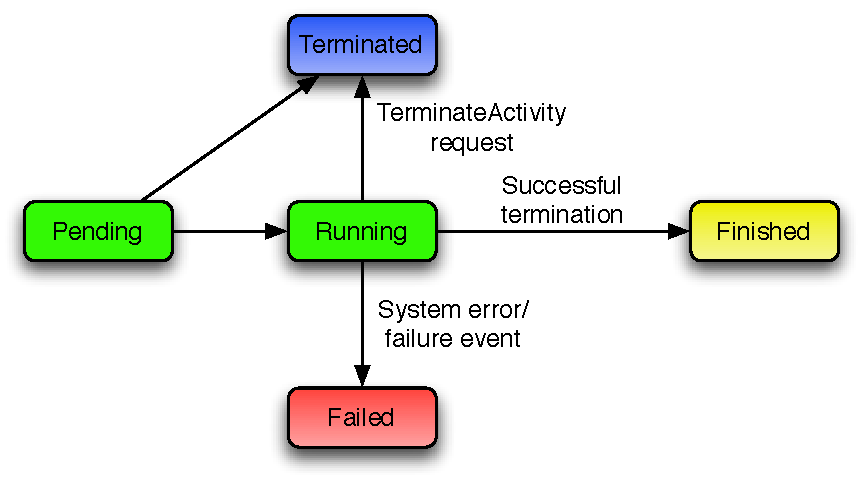
\includegraphics[scale=.6]{bes-basic-job-model}
  \caption[Basic BES Job-State-Model]{This is the job-state-model as it is
    defined in the BES specification \cite{ogsa-bes}}
  \label{fig:bes-basic}
\end{figure}

This very basic state-model represents everything a possible client of the
execution service needs  to know. An actual execution  service may require
to  use  additional  states.   It  can  define both  new  states  and  new
transitions,  as  long  as  it  conforms  to a  rather  simple  rule:  the
\textbf{visual behavior}, as it is experienced by some client, must not be
altered. A breakage of this rule would be the introduction of a transition
from  the \texttt{Running}  state  back into  the \texttt{Pending}  state.
Clearly, the visual behavior a  client experiences, has changed, since the
client  simply  does   not  expect  that  the  activity   is  suddenly  in
\texttt{Pending} again.

\subsection{Extending the state-model}

New states, for  instance, can be added by simply splitting  up one of the
``basic'' states.   Among these sub-states  any number of  new transitions
may be introduced.

Suppose the execution service provides  a way to suspend a given activity.
This  requires  not only  additional  user  requests  --- one  to  request
\emph{suspension} and  one to request  \emph{resumption} --- but  also two
new states. These states are modeled as sub-states of the \texttt{Running}
state, since an  activity may only be suspended  while it already running.
Thus,   the  \texttt{Running}   state   is  now   internally  split   into
\texttt{Executing} and  \texttt{Suspended}. The extended  state machine is
shown in Figure~\ref{fig:bes-suspend-model}

\begin{figure}[h]
  \centering
  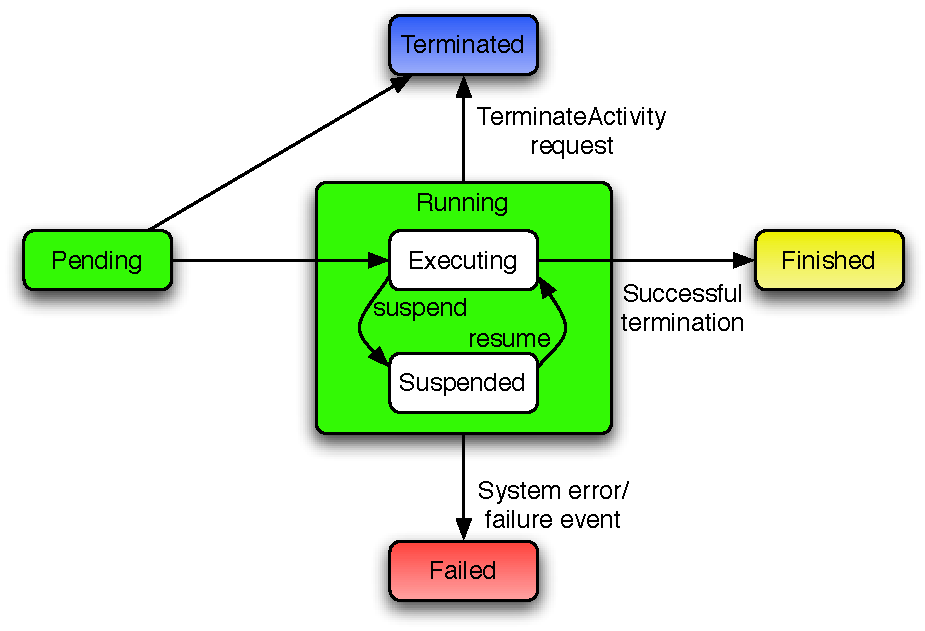
\includegraphics[scale=.6]{bes-suspend-job-model}
  \caption[Extended  BES Job-State-Model]{The  basic state-model  has been
    extended to support suspension.}
  \label{fig:bes-suspend-model}
\end{figure}

The nice  thing about the extensibility  of this state-model  is, that any
client  that  \emph{understands}  the  basic model,  will  understand  any
extended model  as well, that  is because the \emph{visual  behavior} does
not change  and therefore will never ``anything  unexpected'' happen. This
visual  behavior is  directly reflected  in the  XML specification  of the
current state.   Any additional  states are represented  by user-definable
elements attached to  the \texttt{ActivityStatus} element as sub-elements.
Let's  assume   the  extension  modeled   above  defines  its   own  state
representation  using its  own  namespace,  then the  current  state of  a
suspended activity could be written as:

\begin{lstlisting}[language=XML]
  <bes:ActivityStatus state="Running">
     <ext:Suspended/>
  </bes:ActivityStatus>
\end{lstlisting}

As you can see, the state  is still \texttt{Running}, but any client, that
is   aware    of   this   extension,   knows   how    to   interpret   the
\texttt{ext:Suspended} sub-element.

\section[Message Oriented Middleware]{Message Oriented Middleware (MOM)}
\label{sec:fundamentals:mom}

A  typical  way  of connecting  clients  with  some  server  is to  use  a
\gls{glo:TCP}-connection to the server for each client. This is especially
useful if a continuous connection to  the server has to be maintained. For
instance, web (\ie HTTP) and ftp (\ie FTP) servers are usually streaming
a lot of data to the clients.

Communication  in  distributed systems,  however,  can  take place  either
\emph{synchronously}, or  \emph{asynchronously}. The programming  model of
synchronous communication  is called \emph{Remote  Procedure Calls} (RPC),
widespread  implementations  of  this  model  are  CORBA,  RMI  and  DCOM.
Asynchronous   communication  follows   the  emerging   paradigm   of  the
\emph{event-based  communication  model}  \cite{MeCa:2005:Taxonomy}.   The
components that  comprise an application in a  potentially distributed and
heterogeneous   environment   are   asynchronously  interconnected   using
message-passing technologies.

\bigskip

\citet{dad-mom}  state, that  \emph{``Every  DAD (Distributed  Application
  Developer) needs a MOM (Message Oriented Middleware)''}.

Since the communication, which takes  place in the here proposed execution
environment and in  the later discussed Calana Grid  scheduler, is loosely
coupled  and message-oriented,  we  can abstract  from direct  connections
between each party to logical connections.

These logical  connections can be established using  a \gls{glo:MOM} based
on one or more \emph{message-queue servers} (\gls{glo:MQS}).

\gls{glo:MQS}   have  several  very   important  advantages   over  direct
connections between the clients and the server:

\begin{itemize}
\item All messages are  sent to \textbf{logical queues} (\ie end-points),
  that  means   that  the  physical  address  (\eg IP   address)  of  any
  participating  service  (be  it  the  server or  a  client)  may  change
  unnoticeable to the communication partner.
\item All connections are  \textbf{outbound}, which effectively means that
  the server may also reside behind a firewall or a \gls{glo:NAT}-gateway.
  This not only increases the security  of the server (in means of allowed
  inbound  connections),  but  also  targets the  problems  which  typical
  network-policies and  resulting network-layouts of  grid-environments or
  companies impose.
\item The  \gls{glo:MQS} need not  to be on  a single machine, but  can be
  distributed  over  many computers  to  implement \textbf{fail-over}  and
  \textbf{load-balancing}.
\item  Messages  are kept  in  a  \textbf{consistent  storage} within  the
  \gls{glo:MQS}, if they cannot be  delivered right now.  That may happen,
  if the communication partner is temporarily disconnected --- all pending
  messages will be delivered as soon as the end-point connects again.
\item    Multiple   \gls{glo:MQS}   can    be   configured    to   provide
  \textbf{forwarding and  routing} of  messages destined for  a particular
  queue --- that means independence from the actual network-topology.
\item A \gls{glo:MQS} can be configured to provide \textbf{authentication}
  and \textbf{authorization} to limit  access to (\ie send to and receive
  from) particular queues.
\item   Messages   sent   from   one   component   to   another   can   be
  \textbf{transformed}  while passing  the \gls{glo:MQS}.   That  means in
  particular,  that each  component may  send messages  in its  own native
  format and the \gls{glo:MQS}  intelligently transforms the messages into
  the native format of each receiver.
\end{itemize}



\begin{figure}[htbp]
  \centering
  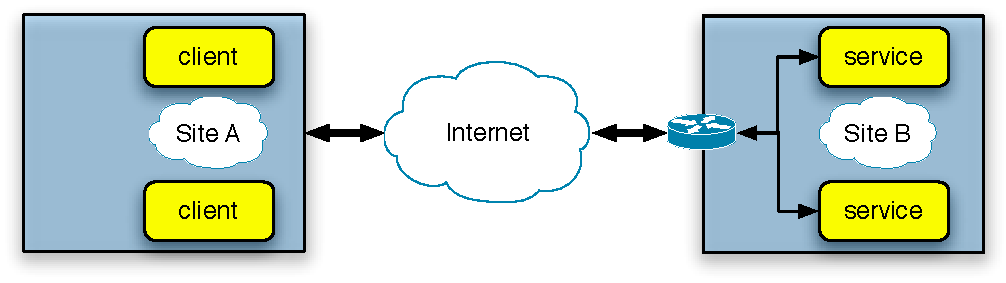
\includegraphics[scale=.5]{mqs-topology}
  \caption[Example MQS topology]{A simple message-oriented system which is
    using a \gls{glo:MQS}.}
  \label{fig:mqs-topology}
\end{figure}

As you can see in  Figure~\ref{fig:mqs-topology}, site B has some services
connected to  a \gls{glo:MQS}.  These services can  be reached  by clients
from site A through an internet connection. The steps involved in building
up this communication scheme are:
\begin{enumerate}
\item  Each service  connects to  the \gls{glo:MQS}  and \emph{subscribes}
  itself to a unique queue (\eg service.\emph{X}).
\item    Clients   subscribe    themselves   to    unique    queues,   too
  (\eg client.\emph{Y}).
\end{enumerate}

Now  that each  party is  subscribed to  its own  unique queue,  a two-way
communication is possible:
\begin{enumerate}
\item A client  that wants to communicate with one  of the services, sends
  its messages  to the unique queue  of that particular  service. The sent
  message  contains a  special \emph{reply-to}  field that  is set  to the
  unique queue of the client
\item Answers from  a service to a connected client are  sent to the queue
  specified in the reply-to field of received messages.
\end{enumerate}

\section{Secure Communication}
\label{sec:secure-communication}

The proposed system  will use message queues to  transfer messages between
clients and the server, that means  all messages that are sent can be read
by any person or system in between any two communication partners. 

A   typical  solution   to  make   the  transfer   secure  is   using  the
\emph{Transport Layer  Security} protocol --- or  \gls{glo:TLS} for short.
\gls{glo:TLS} makes sure that  traffic between two endpoints is transfered
securely --- \ie no eavesdropping, modification or message forgery.

The  \emph{Transport Layer  Security} protocol,  which is  discussed  in a
moment, and the afterwards examined \emph{Message Layer Security} protocol
are  both using cryptographic  certificates such  as \emph{\gls{glo:X509}}
certificates.

The  certificates  are  based  on  public/private  key  pairs,  whereas  a
certificate consists of a  pair's public-key combined with some additional
information, \eg the owner and issuer of the certificate, used algorithms
and  so  on.  Most  importantly  is the  fact,  that  certificates can  be
\emph{cryptographically    signed}     by    a    certificate    authority
(\gls{glo:CA}). The  next passage  will shortly describe  how certificates
can  be  used  in  a  \emph{Public Key  Infrastructure}  using  public-key
cryptography.

\subsection{Public-key cryptography}
\label{sec:fundamentals:public-key}

Public-key  cryptography describes  a form  of cryptography  where  a user
holds  two  different  keys,  a  \emph{private  key}  and  a  \emph{public
  key}.  These two  keys are  mathematically  related to  each other,  but
nobody can practically derive the private key from the public key.

The public key can be made  publicly available without any risk, while the
private key must  be kept very secret. A widely used  algorithm is the RSA
algorithm named  after its  creators \citet*{rivest77method}. It  has been
the first algorithm, that  was suitable for both encryption/decryption and
signing.  For more background information on public-key cryptosystems, you
are encouraged to read \cite{rivest77method,diffie76new}.

The RSA algorithm relies on the fact, that the factorization of reasonably
large numbers is  computationally very hard and no  efficient algorithm is
publicly known.  Especially  hard to factor are numbers  whose factors are
two randomly-chosen prime numbers of sufficient length.

In the following  I am going to describe  how the keys are set  up and how
they are used to encrypt/decrypt or to sign/validate a clear text message.

According  to  \cite{rivest77method},  places  each  user  his  encryption
procedure $E$  in a publicly accessible file  (\eg database).  Using this
public file, any  other user is able to  retrieve the encryption procedure
of   some  other   user  (\ie the   one  he   wants  to   send  encrypted
messages). Each user keeps his decryption procedure $D$ secret.

The mentioned procedures $D$ and $E$ have the following properties:
\begin{enumerate}
\renewcommand{\theenumi}{\alph{enumi}}
\renewcommand{\labelenumi}{(\theenumi)}

\item Deciphering  the enciphered form of  a message $M$  yields $M$. That
  is,
  \begin{equation}
    \label{eq:1}
    D(E(M)) = M.
  \end{equation}
  \label{pubkey-cryptosystem-prop-1}
\item Both $D$ and $E$ are easy to compute.
  \label{pubkey-cryptosystem-prop-2}
\item The user does not reveal an  easy way to compute $D$ if he makes $E$
  publicly available.
  \label{pubkey-cryptosystem-prop-3}
\item  The enciphering  of a  previously ciphered  message $M$  results in
  $M$. That is,
  \begin{equation}
    \label{eq:2}
    E(D(M)) = M.
  \end{equation}
  \label{pubkey-cryptosystem-prop-4}
\end{enumerate}

A                  function                 $E$                 satisfying
(\ref{pubkey-cryptosystem-prop-1})--(\ref{pubkey-cryptosystem-prop-3})   is
said  to  be  a  \emph{``trap-door  one-way function''}  and  if  it  also
satisfies  (\ref{pubkey-cryptosystem-prop-4})  it  is a  \emph{``trap-door
  one-way permutation''} \cite{rivest77method,diffie76new}.

\subsubsection{Key setup}

The \emph{encryption  key} consists  of a pair  of positive  integers $(e,
n)$,  where $e$  is the  \emph{encryption exponent}  and $n$  is  used for
modulo  operations.  The \emph{decryption  key}  is  also  a pair  of  two
integers, where only the exponent differs, thus $(d, n)$ is the decryption
key and $d$  represents the \emph{decryption exponent}. $(e,  n)$ are made
publicly available.

\citet*{rivest77method} suggest the  following approach for the generation
of $(e, n)$ and  $(d, n)$. The fist step is to  compute $n$ as the product
of two very large, ``random'' primes $p$ and $q$:
\begin{equation*}
  \label{eq:compute-n}
n = p \cdot q.
\end{equation*}

Although you  publish $n$, nobody is  able to compute the  factors $p$ and
$q$ in  reasonably time due to  the enormous difficulty  of factoring $n$.
In \cite{rivest77method}  it is assumed,  that the computation of  $p$ and
$q$ from a given $n$ takes $1.5 \times 10^{29}$ operations, given that $n$
has a length  of $300$ digits. If one operation  took one microsecond, the
whole computation takes $4.9 \times 10^{15}$ years.

The  next step  is to  choose  $d$, therefore  one picks  a large,  random
integer that is \emph{co-prime}\footnote{two integers $a$ and $b$ are said
  to be co-prime  if they do not  have a common factor other  than $1$ and
  $-1$, \ie their greatest common divisor  (gcd) is $1$.} to $(p-1) \cdot
(q-1)$.\footnote{the term $(p-1)\cdot(q-1)$ is the result of \emph{Euler's
    Phi} or  \emph{Euler's totient function}  ($\phi$) applied to  $n$} In
other words, $d$ has to satisfy:
\begin{equation*}
  \label{eq:compute-d}
  gcd(d, (p-1) \cdot (q-1)) = 1.
\end{equation*}

Finally,  the integer $e$  is computed  from $p$,  $q$ and  $d$ to  be the
\emph{multiplicative inverse} of $d$, modulo $\phi(n)$:
\begin{equation*}
  \label{eq:compute-e}
  e \cdot d \equiv 1\ \ (mod\ (p-1) \cdot (q-1))
\end{equation*}

\subsubsection{Encryption and Decryption}

If  two  persons,  Alice  and   Bob,  want  to  send  each  other  private
(\ie encrypted)  messages,  they   both  retrieve  the  other's  publicly
available encryption  key first ---  Bob retrieves $(e_a, n_a)$  and Alice
retrieves $(e_b, n_b)$.

Let's say  Alice wants to send a  private message to Bob.   To encrypt the
message, she has to  represent it as an integer between $0$  and $n_b - 1$
(long  messages can  be broken  into smaller  blocks, so  that  each block
fulfills the requirement). Alice then  encrypts the message $M$ by raising
it to the $e_b$th power modulo $n_b$, the result is the cyphertext $C$:
\begin{equation*}
  \label{eq:encrypt-message}
  C \equiv E(M) \equiv M^{e_b}\ \ (mod\ \ n_b).
\end{equation*}

On reception  of the cyphertext  $C$, Bob raises  it to the  $d_b$th power
modulo $n_b$. He  is the only person, who knows $d_b$  and therefore he is
solely able to decrypt $C$:
\begin{equation*}
  \label{eq:decrypt-message}
  M \equiv D(C) \equiv C^{d_b}\ \ (mod\ \ n_b).
\end{equation*}

\subsubsection{Signing and Validating}

Electronic  signatures, \eg in electronic  mail systems,  especially when
used in  business transactions, must  provide provability to  the receiver
that  the message  originated from  the sender.   This is  more  than just
provide  mere \emph{authentication},  where the  recipient of  a digitally
signed message can  verify that the message came  from the sender. Digital
signatures must be  able to be used to convince  a ``judge'', that neither
the recipient did  forge the message, nor the sender  can deny sending the
message.

That means,  an electronic signature must  be \emph{message}-dependent, as
well as  \emph{signer}-dependent. If the  signature did not depend  on the
message itself, a dishonorable recipient  could just change the message or
attach the signature to a  completely different message before showing the
message/signature pair  to a judge. If  the signature would  not depend on
the \emph{signer}, obviously anybody could have signed the message.

\medskip

If   Bob  want  to   send  Alice   a  signed   message,  he   applies  his
\emph{decryption}  function $D_b$  to the  clear text  message  $M$, which
results in the signature $S$:

\begin{equation*}
  \label{eq:compute-signature}
  S = D_b(M).
\end{equation*}

To   perform  this,   the  cryptosystem   has  to   be   implemented  with
\emph{trap-door         one-way        permutations},        \ie property
(\ref{pubkey-cryptosystem-prop-4}) must hold.

This signature  can now  be encrypted using  Alice's public key  to ensure
privacy, there  is no need to  send the message along  with the signature,
since it can  be computed from it. On reception,  Alice first decrypts the
message which  results in the  plain signature $S$ again.   Applying Bob's
\emph{encryption} function to the  received signature (Alice knows who the
presumed sender  of the  message is) makes  perfect sense due  to property
(\ref{pubkey-cryptosystem-prop-4}):

\begin{equation*}
  \label{eq:validate-signature}
  M = E_b(S)
\end{equation*}

Bob cannot  later on deny that he  sent the message, since  nobody but him
could  have generated  the signature  $S$.  Alice  is able  to  convince a
``judge'', that  Bob did send the  message, since $E_b(S) =  M$. But Alice
cannot modify  $M$ or  provide a different  message $M'$ because  then she
would also need to compute $S' = D_b(M')$ as well.

\subsection[Public Key Infrastructure]{Public Key Infrastructure (PKI)}

A  \emph{Public Key  Infrastructure} provides  the authentication  of user
identities using certificates.  The main  aspect is that there are special
\textbf{trusted    third     parties}    (\emph{Certificate    Authority},
\gls{glo:CA}), that are permitted  to \textbf{sign} other certificates. If
a  user\footnote{or some  server, etc.}   wants to  prove his  identity to
another entity,  his certificate is  validated by that entity  against the
CA's certificate, if it is valid, the prove has been successful.

The \gls{glo:CA} is responsible for checking that the public-key contained
in  the certificate  actually belongs  to the  requesting user,  server or
other  entity denoted  in the  certificate. This  checking process  is for
example done by  verifying the credentials of a user  (\eg with help of a
photo identification or something similar).

Any third-party that trusts a given CA will transparently trust any entity
that offers a certificate signed by that particular CA.

\begin{figure}[h]
  \centering
  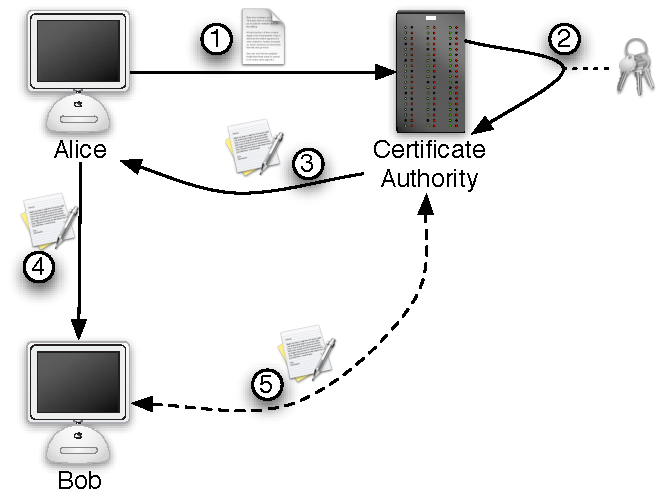
\includegraphics[scale=.75]{pki}
  \caption[Public  Key Infrastructure]{Alice  proofs her  identity  to Bob
    using a certificate  that is signed by a CA that  both, Alice and Bob,
    trust.}
  \label{fig:pki}
\end{figure}

Validation is performed by verifying  that the certificate itself has been
signed  by a  trusted authority  --- the  actual validation  process  is a
little   bit  more  complex,   since  it   involves  checking   against  a
\emph{Revocation List} and  a ``best before'' date (\ie life  time of the
certificate), too.

The  signing  process  uses  the  authority's private  key  to  compute  a
cryptographic signature. This private-key must of course be kept in a very
secure  location  (\eg on a  physically  from  the Internet  disconnected
computer) ---  if it would fall into  the wrong hands, the  whole chain of
trust is compromised.

An  example verification  process  is shown  in Figure~\ref{fig:pki},  the
steps can be described as follows:
\begin{enumerate}
\item \emph{Alice} request the signing of her certificate by a CA and thus
  sends a certificate request to the CA containing her public-key.
\item The CA in turn verifies Alice's credentials and eventually signs the
  certificate with its private key.
\item The signed certificate is sent back to \emph{Alice} for her later use.
\item Now,  \emph{Alice} wants to prove  her identity to a  friend of her,
  \emph{Bob},   therefore   \emph{Alice}    sends   her   certificate   to
  \emph{Bob}.  The   proof  may  be   necessary  to  establish   a  secure
  communication over an insecure channel, \eg the Internet.
\item \emph{Bob}  verifies the received certificate against  the very same
  CA by  which \emph{Alice} had her certificate  signed.  Since \emph{Bob}
  trusts the  CA and the received  certificate states, that  it belongs to
  his  friend \emph{Alice},  he  can be  assured,  that he  is talking  to
  \emph{Alice}.
\end{enumerate}

\bigskip

Both  of  the following  protocols  can make  use  of  a \gls{glo:PKI}  to
authenticate communication partners.

\subsection[Transport Layer Security]{Transport Layer Security (TLS)}
\label{sec:fundamentals:tls}

The \gls{glo:TLS}  protocol is often  offered by web- or  email-servers to
make  the  communication   with  a  client  (such  as   a  browser  or  an
email-client) secure.

On-line   banking,   for   instance,   typically   requires   a   Personal
Identification Number  (PIN) to make sure  that it is actually  you who is
trying to access your accounts.  Using unencrypted transfer of the PIN and
other data would mean, that any  system, which is in between your computer
and the  one of your  bank, is  able to read  your PIN and  probably other
information about you. It is also possible that a \emph{man-in-the-middle}
spoofs or modifies  transactions to withdraw money from  your account. Two
things are  very important in  this case: The  first and most  obvious is,
that the information you and  your bank exchange are encrypted. The second
requirement is,  that you  are able  to verify that  the receiver  of your
messages is actually a computer belonging  to your bank and not to someone
else.

\gls{glo:TLS} uses  certificates on the  server-side, so that  clients can
validate  that  they  are  actually  communicating with  the  server  they
intended to  communicate with.  In  the case of  a bank or  any well-known
service  provider   in  the  Internet,  the  certificates   in  place  are
cryptographically  signed by a  \emph{trusted} authority.   A certificate,
that is signed by such an authority you trust, is automatically assumed to
actually belong to the server where the certificate came from.

\bigskip

Unfortunately, \gls{glo:TLS}  cannot be used in a  message-queue system to
secure the traffic  between clients and servers. That  is because there is
no direct connection between client and server --- both are just connected
to their message-queue server. \gls{glo:TLS} can in this case only be used
to secure  the communication between  any end-point and  the message-queue
server it  is connected to.

After transmitting a message over a with \gls{glo:TLS} secured connection,
the  message is  stored in  clear text  on the  message-queue  server. The
message   will  then   again  be   transmitted  securely   to   the  final
destination. But  any person  or system with  access to  the message-queue
server can read, modify or even spoof transmitted messages --- without the
knowledge of either sender or receiver.

To  secure  the  logical   message-based  communication  between  any  two
end-points, a  different kind of security  layer has to be  used here: the
\emph{Message Layer Security} --- or \gls{glo:MLS} for short.

\subsection[Message Layer Security]{Message Layer Security (MLS)}
\label{sec:fundamentals:mls}

As the name of this protocol  may already suggest, the security focuses on
the transmitted messages not on  the transportation of the messages.  That
means, the transport layer over which  messages are sent is not altered or
secured in any way  --- it can be as insecure as  before.  But even though
the messages are transmitted over a potentially insecure channel, they are
still protected against eavesdropping, tampering and spoofing.

\gls{glo:MLS} too makes use  of certificates to provide authentication and
encryption. To  establish a  secure communication between  a client  and a
server,  the  client  needs  to  \emph{know}  (\ie have  access  to)  the
certificate  of the server.   Since encryption  with a  public/private key
algorithm   is    rather   slow,    in   most   cases    a   \emph{session
  key}\footnote{typically  random data}  will be  negotiated  first.  This
session  key is  then used  to perform  \emph{symmetric} ciphering  of the
messages, which is a lot faster.

\bigskip

The \gls{glo:XenBEE}  must make use  of \gls{glo:MLS} to  provide security
for  its users.   Additionally, as  it is  common  among Grid-middlewares,
\gls{glo:X509}  certificates  are   used  to  authenticate  and  authorize
users. The  server is going  to use a  user's certificate to  validate his
identity and  possibly to send messages  the user --- thus  both sides may
initiate a secure communication.

\section{Calana}
\label{sec:calana}

\emph{Calana} is  a new Grid  scheduler approach proposed  by M.~Dalheimer
\cite{dalheimer05agentbased}.  The  scheduler uses \emph{agents}  that are
responsible for  a single  resource and at  least one  \emph{broker}.  The
broker initiates an \emph{auction} among  the connected agents to assign a
task to some resource.

\begin{figure}[htbp]
  \centering
  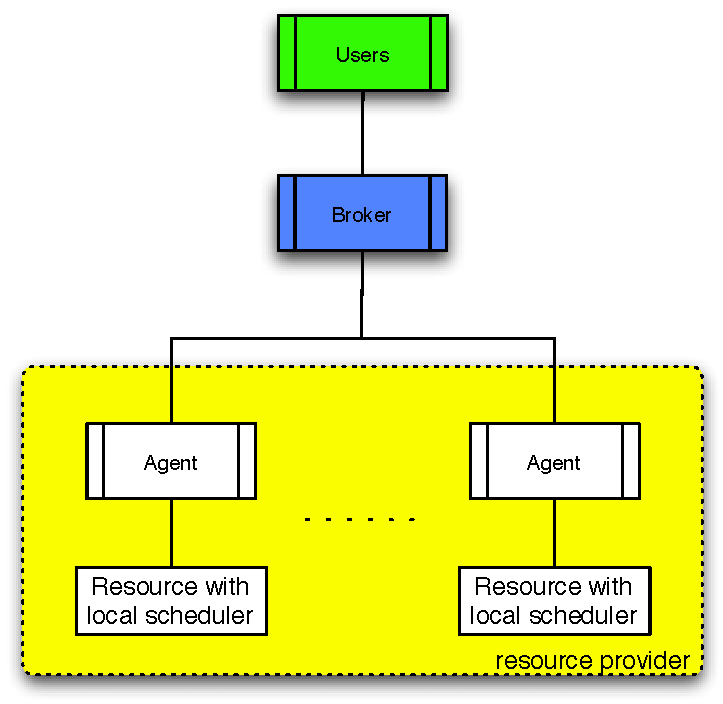
\includegraphics[scale=0.5]{calana-architecture}
  \caption{Architecture of Calana}
  \label{fig:calana-architecture}
\end{figure}

An  abstract   view  over   the  architecture  of   Calana  is   shown  in
Figure~\ref{fig:calana-architecture}.   For a  detailed discussion  of the
Calana-protocol  that  is used  to  perform an  auction,  have  a look  at
\cite{dalheimer06calanaprotocol,petry06}, but  the  main steps  involved
are:
\begin{enumerate}
\item When a user submits a job to the Calana-broker, the broker will open
  up an auction and try to \emph{book} a resource for the task.
\item    For   each   task    an   auction    is   created    by   sending
  \texttt{BookingReq}-messages to the connected agents.
\item The agents will make  one or more \emph{reservations} on their local
  scheduler  and  answer with  a  \texttt{AuctionBid}.   Bids contain  for
  example  the  cost  of   using  the  resource  and  various  reservation
  parameters  such  as  the   earliest  start-time  and  duration  of  the
  reservation.
\item To make a decision, the  broker judges all received bids and chooses
  the     best     one      according     to     some     preference-model
  \cite{dalheimer05agentbased, petry06}.
\item If  the user  accepts the decision,  the broker  \emph{confirms} the
  reservation.
\end{enumerate}

%%% Local Variables: 
%%% mode: latex
%%% TeX-master: "main.tex"
%%% End: 

\chapter{Requirements}
\label{cha:requirements}

This  work deals  with  an  execution environment  that  uses Xen  virtual
machines to run  applications in a secure environment.   In this chapter I
am going to describe, how such an environment can look like and what it is
supposed to provide the users with.

\begin{figure}[htbp]
  \begin{center}
    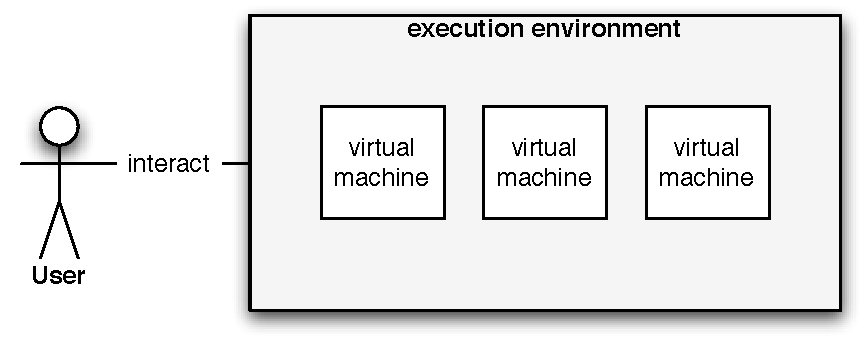
\includegraphics[scale=.5]{concept}
  \end{center}
  \caption[Conceptual overview]{A conceptual overview}
  \label{fig:concept}
\end{figure}

In Figure~\ref{fig:concept},  a conceptual overview  is shown, it  depicts a
single user interacting with the execution environment.

The next sections describe what  I think, an execution environment must at
least provide to be useful. Furthermore, several use-cases are given, that
show possible usage scenarios of the execution environment.

\section{Execution environment}
\label{sec:req-execution-environment}

What should an execution environment  provide, so that users can work with
it?  I  think  the following  list  gives  a  good  idea about  the  basic
requirements any execution environment should fulfill:

\begin{itemize}
\item \emph{Submit new tasks} --- i.e.~inform the system about a new task,
  that it should execute.
\item \emph{Query the status of  tasks} --- i.e.~is the task still pending
  and  waiting for  its execution,  currently  running or  did it  already
  finish.
\item \emph{Stop running tasks} --- i.e.~a user must always have the
  possibility to cancel his own tasks.
\end{itemize}

Typically, tasks  require some input data  to work on  and generate output
data  ---  to describe  such  tasks  we  demand the  following  additional
requirements:
\begin{itemize}
\item Provide a way to specify input data for a task
\item Provide a way to retrieve generated output data from a task
\end{itemize}

The next sections describe each point in more detail --- they also explain
specifications  such  as the  \emph{Job  Submission Description  Language}
(\gls{glo:JSDL}) \cite{jsdl-spec}  and the \emph{Basic  Execution Service}
(\gls{glo:BES}) \cite{ogsa-bes}.

\subsection{Submission of tasks}
\label{sec:req-task-submission}

In  grid environments,  for example,  the user  describes his  job  as the
application he wants to execute,  additional parameters that are passed to
the application, input and output data and many more.

The here proposed execution environment demands a way to describe not only
the tasks, but also  the virtual machine that is going to  be used for the
task.

An upcoming standard for a job description, that is not restricted to grid
environments, but  can be used  in various environments, is  the \emph{Job
  Submission  Description  Language}   ---  or  \gls{glo:JSDL}  for  short
\cite{jsdl-spec}.

I  decided to  use this  description language,  so that  the Xen-execution
environment can  easily be integrated  into various middlewares  that also
use the \gls{glo:JSDL} to describe their jobs.

\subsubsection{Job Submission Description Language (\gls{glo:JSDL})}

\gls{glo:JSDL}  is a  very extensible  XML-based description  language for
computational  jobs.  With  \gls{glo:JSDL} you  are able  to  describe all
requirements that  a computational  job may need  for the submission  to a
resource --- mainly the \gls{glo:JSDL}  addresses grid resources but it is
not limited the latter.

\paragraph{The building   blocks}

A  \gls{glo:JSDL}   document  always  contains   a  \texttt{JobDefinition}
element, which is the top-level element and holds all required information
about the job.

A  minimalistic  example is  shown  in Listing~\ref{lst:jsdl-example},  it
describes the execution of the following command in a standard UNIX shell:

\begin{minipage}{0.75\textwidth}
  \begin{lstlisting}[language=ksh]
    $ echo Hello World
    Hello World
    $
  \end{lstlisting}
\end{minipage}

\lstinputlisting[float=ht,caption={A small ``Hello World''-example written in \gls{glo:JSDL}},label={lst:jsdl-example},language=XML]{examples/jsdl-example.jsdl}

\bigskip

A typical \gls{glo:JSDL} document consists  of the following parts --- job
identification,  application description,  resource descriptions  and data
staging elements:

\begin{description}
\item[\emph{JobIdentification}] This element  is used to hold information
  about the job that is mostly  interesting for human beings --- such as a
  descriptive  name  for the  job.   Nonetheless  it  may hold  additional
  information  that  could  be  of  interest to  machines  processing  the
  document  --- such  as  annotations (e.g.~a  unique task  identification
  number can be stored in such an annotation).
\item[\emph{Application}] With this element,  a user describes the program
  itself  --- i.e.~the real  executable, that  is to  be used.   A special
  extension   ---   \texttt{POSIXApplication},   also   defined   in   the
  specification \cite{jsdl-spec}  --- can be used  to describe executables
  for    \gls{glo:POSIX}-compliant    operating   systems    \cite{posix}.
  Listing~\ref{lst:jsdl-example}   uses  this   element  to   execute  the
  \texttt{echo} program.
\item[\emph{Resources}]  This  element can  be  used  to describe  various
  resource requirements  of the  application. Some examples  for resources
  are:
  \begin{itemize}
  \item the number of CPUs the job requires
  \item the operating system required by the job
  \item amount of virtual memory that must be available for the job
  \item file-systems and their mount-points that have to be made available
    for the job
  \end{itemize}
  The file-system definitions  are placeholder variables for \emph{logical
    places} within  the file-system hierarchy.  They can be used  in other
  elements to refer to some file ``below'' a particular file-system.
\item[\emph{DataStaging}]   The   \texttt{DataStaging}   element  can   be
  specified  arbitrarily often  and  defines both  stage-in and  stage-out
  operations.   A stage-in operation  is a  file-transfer that  must occur
  prior executing  the job (i.e.~it prepares  the input data  for the job)
  and obviously stage-out operations take place after the job has finished
  its execution.

  The  most relevant  elements within  a DataStaging  instruction  are the
  \texttt{Source} and \texttt{Target} elements ---  both can hold a URI to
  specify a  generic location ---  and the \texttt{FileName} element which
  points to an actual file within the file-system hierarchy.
\end{description}

As you  can see, the \gls{glo:JSDL}  is really powerful and  it covers all
requirements  a typical computational  job may  have. And  if it  does not
cover a  special topic, one  is able to  extend the defined  elements with
custom elements.

\subsubsection{Extensions to the \gls{glo:JSDL}}

To be able to create a virtual machine on the remote site, the user has to
specify not only  the application she wants to run  but also a file-system
\gls{glo:image}  that  contains  an  operating system  installation.   The
execution environment then  takes care of starting up  the virtual machine
with  the  provided  \gls{glo:image}   and  will  eventually  execute  the
application.

The  description  of a  virtual  machine cannot  be  done  using only  the
\gls{glo:JSDL},  since one has  to describe  additional locations  for the
\gls{glo:image}, a  kernel and probably an initial  RAM-disk.  Those files
are not directly  related to the description of a job  and one cannot just
use  \texttt{DataStaging}  elements, since  they  act  on the  file-system
hierarchy seen from the job's  point of view, i.e.~from within the virtual
machine.   The extensions  made  to the  \gls{glo:JSDL}  are discussed  in
chapter \ref{cha:design} in more detail.

\subsection{Query the status of tasks}
\label{sec:status-query}

A user  who submitted a task  to some remote system  for execution, surely
wants to observe the current state of his job. The query for the status of
a   job  requires  the   detailed  specification   of  which   states  are
\textbf{allowed  states}  and  how  the \textbf{transitions}  between  the
states look like.

To provide  the possibility to connect the  Xen-execution environment with
other  tools,  a  common  description  for job-states  is  required.   The
\emph{Open Grid Services Architecture} (\gls{glo:OGSA}, \cite{ogsa}) has a
working group which designs such a common state model for job execution in
grid environments  --- the \emph{Basic  Execution Service} (\gls{glo:BES},
\cite{ogsa-bes}).

The OGSA is an approach to  use Web service concepts and technologies in a
Grid  environment. Consequently, the BES defines a Web service, but I will
just make use of the generic job-state-model they define.

\subsubsection{The \gls{glo:BES} state-model}

The  specification  for  the  \gls{glo:BES}  contains  a  very  extensible
state-model for job execution.  The basic model just defines five distinct
states      \texttt{Pending},     \texttt{Running},     \texttt{Finished},
\texttt{Failed} and \texttt{Terminated} ---  the state-model and its valid
transitions are shown in Figure~\ref{fig:bes-basic}.

\begin{figure}
  \begin{center}
    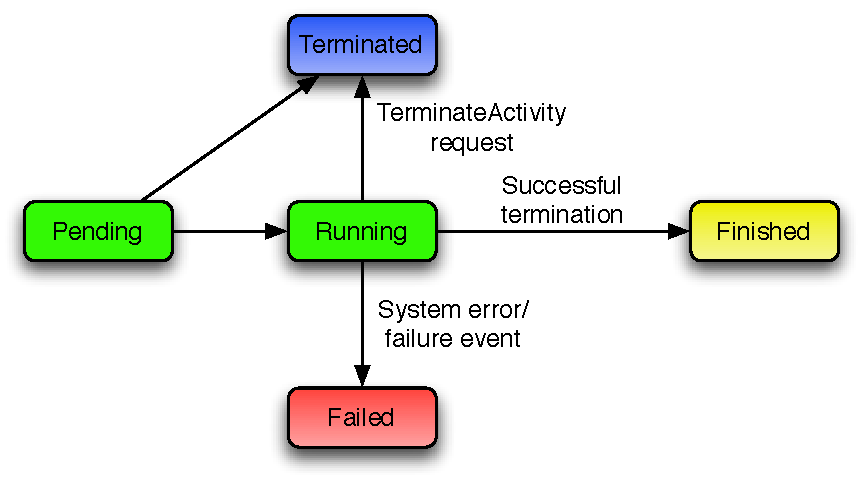
\includegraphics[scale=.75]{bes-basic-job-model}
  \end{center}
  \caption[Basic BES Job-State-Model]{This is the job-state-model as it is
    defined in the BES specification \cite{ogsa-bes}}
  \label{fig:bes-basic}
\end{figure}

A real  application can  specialize this state-model  for its own  use and
define new states and transitions as long as the \textbf{visual behaviour}
stays the same as of the basic state-model --- i.e.~no transitions must be
added that would not be allowed in the basic model.

The nice  thing about the extensibility  of this state-model  is, that any
client that  \emph{understands} the basic model,  will understand extended
model as  well, that  is because  the outer behaviour  did not  change and
therefore ``nothing unexpected'' ever happens.

\subsubsection{Extensions to the BES state-model}

Since the basic  \gls{glo:BES} state-model is a very  minimal one, we need
to  extend   it  to  allow   the  description  of   data-transfer  states.
Fortunately,  the \gls{glo:BES}  provides such  an extended  model  in its
specification, it is shown in Figure~\ref{fig:bes-extended}.

\begin{figure}
  \begin{center}
    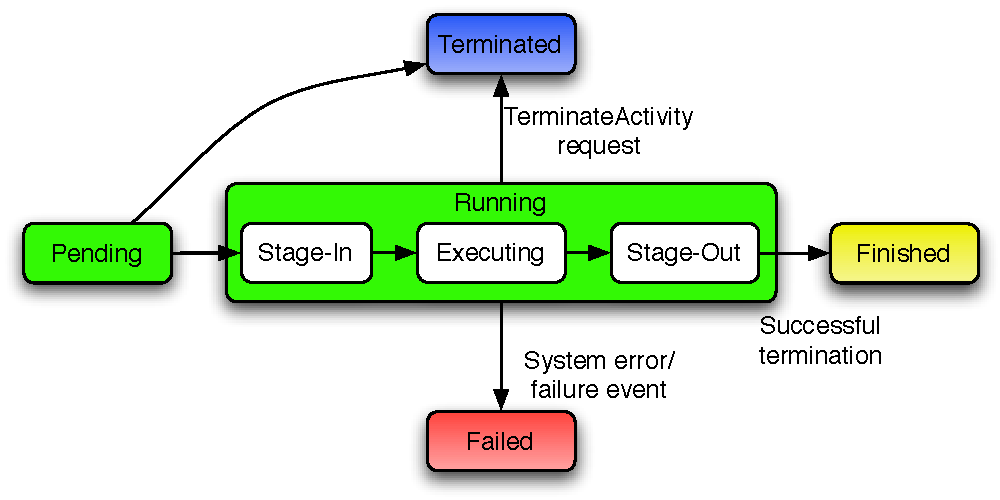
\includegraphics[scale=.75]{bes-staging-job-model}
  \end{center}
  \caption[BES State Model Staging Extension]{The basic BES state-model
    extended with sub-states to describe data-transfers.}
  \label{fig:bes-extended}
\end{figure}

The  \texttt{Running}   state  has   been  split  into   three  sub-states
\texttt{Stage-In}, \texttt{Stage-Out} and \texttt{Executing} --- the first
two describe data-transfer operations and the last one describes the state
in which the task is  actually being executed.  An invalid specialization,
for  example,  would   have  been  the  addition  of   a  transition  from
\texttt{Running:Stage-In} back  to \texttt{Pending}, since  that behaviour
is impossible in the basic state-model.

The  \gls{glo:BES}  specification  as  it  is for  the  JSDL,  defines  an
XML-Schema,  that is  to  be  used for  state  description. The  following
example shows  you the usage  of the state  description using XML  and how
specialized sub-states are represented. The main state is \texttt{Running}
and is  described using the \emph{ActivityStatus}  element, any sub-state,
that may currently be active,  depends on the application and therefore is
described using one or more elements from a different namespace.

\begin{minipage}{0.75\textwidth}
  \begin{lstlisting}[language=XML]
    <bes:ActivityStatus state="Running">
       <n00:Stage-In/>
    </bes:ActivityStatus>
  \end{lstlisting}
\end{minipage}

The example  makes use of  the previously defined  specialized state-model
and  describes an  activity  that is  currently  in the  \texttt{Stage-In}
sub-state of \texttt{Running} --- i.e.~it is waiting for its input data to
be  ready.  Any  client  which  is  not  aware  of  the  \texttt{Stage-In}
sub-state, will only ``see'' that  the activity is in the \texttt{Running}
state.


\subsection{Stopping tasks}
\label{sec:stopping-task}

As  you can  see in  Figure~\ref{fig:bes-extended}, each  non-terminal state
provides  a transition  to  the state  \texttt{Terminated}. That  directly
resembles the requirements for \emph{stopping a task} on user request.

In  case of  this work,  stopping  a task  may involve  shutting down  the
virtual  machine,  terminating active  data  transfers  and releasing  any
acquired resources.

\section{A more concrete concept}

This  section   outlines  a  more  concrete  concept   for  the  execution
environment and its  components. We are going to need  a component that is
responsible for  the requests a  user makes to the  execution environment,
this component  is also going to  manage the virtual machines  for each of
the tasks.

\begin{figure}[htbp]
  \begin{center}
    \begin{minipage}{.75\textwidth}
      \begin{center}
        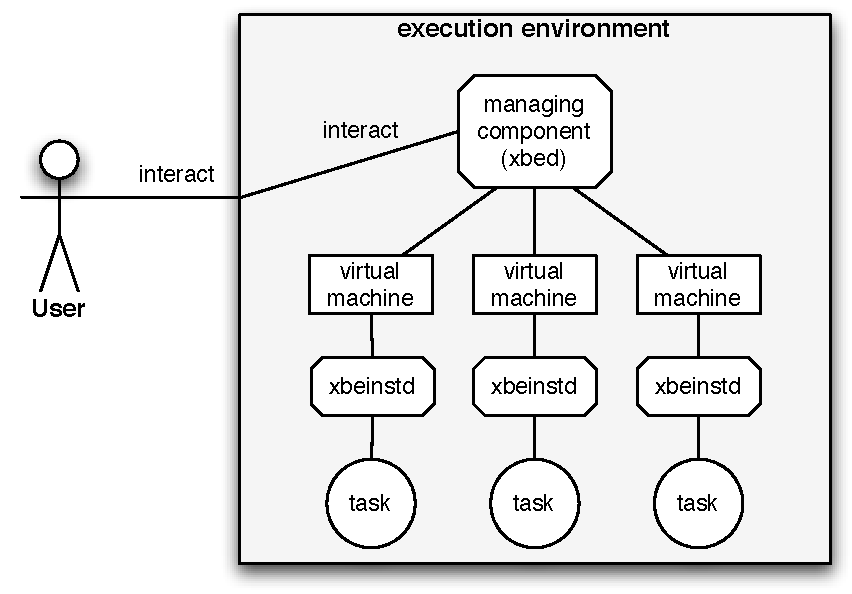
\includegraphics[scale=.5]{concrete-concept}
      \end{center}
      \caption[A  more  concrete  concept]{The  evolved concept,  using  a
        managing component to control  the virtual machines.  Each virtual
        machine  is   dedicated  to  a  single  task   submitted  by  some
        user. Users only interact with the managing component.}
      \label{fig:concrete-concept}
    \end{minipage}
  \end{center}
\end{figure}

Basically  this concept  defines a  client-server architecture,  where the
client is represented  by the user (or some mediator  such as a web-portal
or a  command-line client) and the  server is represented  by the managing
component.

The following  sections motivate the communication  architecture, which is
used  to connect up  clients and  the managing  component, and  a detailed
description of how the tasks should be handled.

\subsection{Basic communication architecture}
\label{sec:basic-communcation-architecture}

A  typical  way  of connecting  clients  with  some  server  is to  use  a
\gls{glo:TCP}-connection  to  the  server  for  each  client.   Since  the
communication which  takes place  in this environment  is message-oriented
--- as  you will  see later,  each request to  the server  is mapped  to a
single  XML document  ---  we can  abstract  from a  direct connection  to
logical  connection.  This  logical  connection can  be established  using
\emph{message-queue servers} (\gls{glo:MQS}).

\gls{glo:MQS}   have  several  very   important  advantages   over  direct
connections between the clients and the server:

\begin{itemize}
\item All messages are  sent to \textbf{logical queues} (i.e.~end-points),
  that  means   that  the  physical  address  (e.g.~IP   address)  of  any
  participating  service  (be  it  the  server or  a  client)  may  change
  unnoticeable to the communication partner.
\item All connections are  \textbf{outbound}, which effectively means that
  the server may also reside behind a firewall or a \gls{glo:NAT}-gateway.
  This not only increases the security  of the server (in means of allowed
  inbound  connections),  but  also  targets the  problems  which  typical
  network-policies and  resulting network-layouts of  grid-environments or
  companies impose.
\item The  \gls{glo:MQS} need not  to be on  a single machine, but  can be
  distributed  over  many computers  to  implement \textbf{fail-over}  and
  \textbf{load-balancing}.
\item  Messages are  stored within  the \gls{glo:MQS},  if they  cannot be
  delivered right now.   That may happen, if the  communication partner is
  temporarily disconnected  --- all pending messages will  be delivered as
  soon as the end-point connects again.
\item Multiple  \gls{glo:MQS} can be  configured to provide  forwarding of
  messages  destined for a  particular queue  --- that  means independence
  from the actual network-topology.
\item A \gls{glo:MQS} can be configured to provide \textbf{authentication}
  and \textbf{authorization} to limit  access to (i.e.~send to and receive
  from) particular queues.
\end{itemize}

\begin{figure}[htbp]
  \begin{center}
    \begin{minipage}{.75\textwidth}
      \begin{center}
        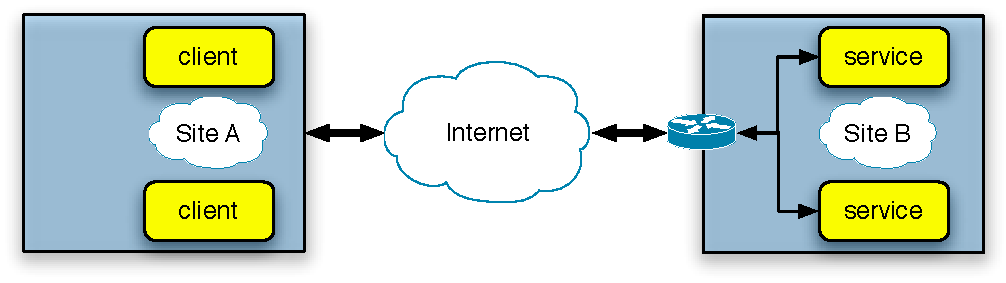
\includegraphics[scale=.5]{mqs-topology}
      \end{center}
      \caption[Example MQS topology]{A simple message-oriented system
        which is using a \gls{glo:MQS}.}
      \label{fig:mqs-topology}
    \end{minipage}
  \end{center}
\end{figure}

As you can see in  Figure~\ref{fig:mqs-topology}, site B has some services
connected to  a \gls{glo:MQS}.  These services can  be reached  by clients
from site A through an internet connection. The steps involved in building
up this communication scheme are:
\begin{enumerate}
\item  Each service  connects to  the \gls{glo:MQS}  and \emph{subscribes}
  itself to a unique queue (e.g.~service.\emph{X}).
\item    Clients   subscribe    themselves   to    unique    queues,   too
  (e.g.~client.\emph{Y}).
\end{enumerate}

Now  that each  party is  subscribed to  its own  unique queue,  a two-way
communication is possible:
\begin{enumerate}
\item A client  that wants to communicate with one  of the services, sends
  its messages  to the unique queue  of that particular  service. The sent
  message  contains a  \emph{reply-to} field  which is  set to  the unique
  queue of the client.
\item Answers from  a service to a connected client are  sent to the queue
  specified in the reply-to field of received messages.
\end{enumerate}

\section{Support for Calana}
\label{sec:calana-support}

\emph{Calana} is  a new  Grid-scheduler approach proposed  by M.~Dalheimer
\cite{dalheimer05agentbased}.  The  scheduler uses \emph{agents}  that are
responsible for  a single  resource and at  least one  \emph{broker}.  The
broker initiates an \emph{auction} among  the connected agents to assign a
task to some resource.

\begin{figure}[htbp]
  \begin{center}
    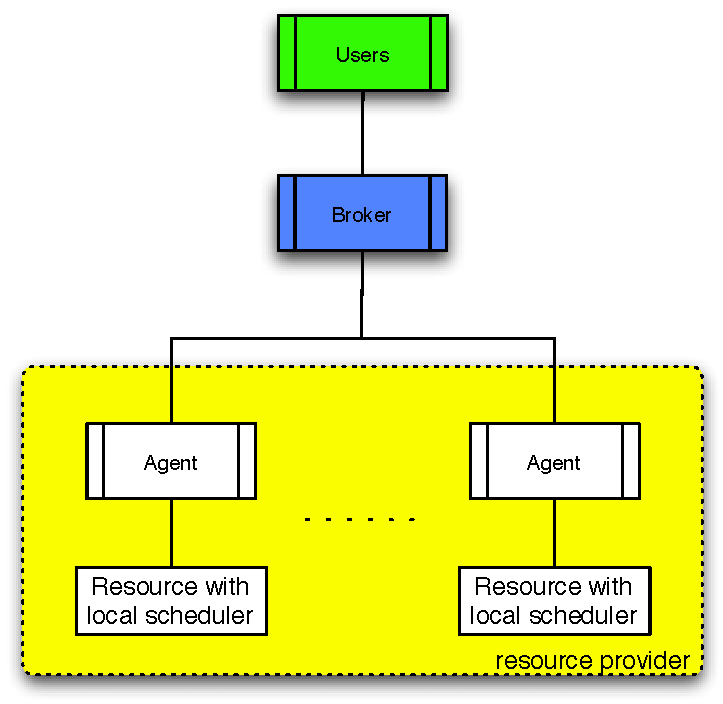
\includegraphics[scale=0.5]{calana-architecture}
  \end{center}
  \caption{Architecture of Calana}
  \label{fig:calana-architecture}
\end{figure}

An  abstract   view  over   the  architecture  of   Calana  is   shown  in
Figure~\ref{fig:calana-architecture}.   For a  detailed discussion  of the
Calana-protocol  that  is used  to  perform an  auction,  have  a look  at
\cite{dalheimer06calanaprotocol,petry06}, but  the  main steps  involved
are:
\begin{enumerate}
\item When a user submits a job to the Calana-broker, the broker will open
  up an auction and try to \emph{book} a resource for the task.
\item    For   each   task    an   auction    is   created    by   sending
  \texttt{BookingReq}-messages to the connected agents.
\item The agents will make  one or more \emph{reservations} on their local
  scheduler  and  answer with  a  \texttt{AuctionBid}.   Bids contain  for
  example  the  cost  of   using  the  resource  and  various  reservation
  parameters  such  as  the   earliest  start-time  and  duration  of  the
  reservation.
\item To make a decision, the  broker judges all received bids and chooses
  the     best     one      according     to     some     preference-model
  \cite{dalheimer05agentbased, petry06}.
\item If  the user  accepts the decision,  the broker  \emph{confirms} the
  reservation.
\end{enumerate}

To  support  Calana, the  \gls{glo:XenBEE}  must  provide some  additional
functionality. One of these functionalities is a mechanism to \emph{make},
\emph{cancel}   and   \emph{confirm}   reservations.   To   reflect   that
requirement, we discussed about a common state-model for the jobs and came
to the consensus of adopting the \gls{glo:BES} model to our needs.

The implementation of Calana, which is currently still in development, too
uses message queues to implement the communication between the brokers and
the agents.

\begin{figure}[htbp]
  \begin{center}
    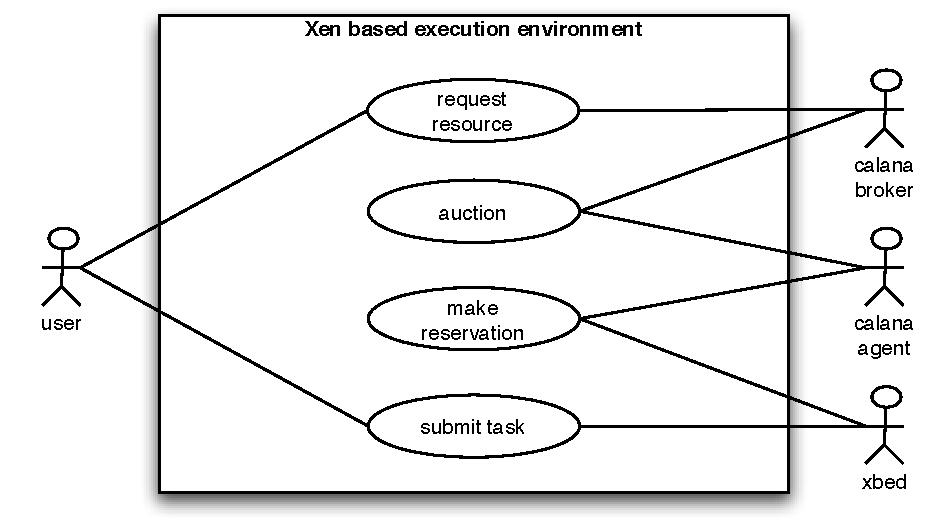
\includegraphics[scale=0.7]{uc-calana-xenbee}
  \end{center}
  \caption[Calana and  XenBEE]{The actors and use cases  that are involved
    when a Calana agent uses the \gls{glo:XenBEE} as its resource.}
  \label{fig:calana-xenbee}
\end{figure}

The picture  in Figure~\ref{fig:calana-xenbee} describes how  a user would
interact  with  a  system,  that   uses  Calana  for  scheduling  and  the
\gls{glo:XenBEE} as  its execution environment. The user  first requests a
resource from  the broker, who in turn  will open up an  auction among the
agents.   One of  those  agents are  shown  in the  figure,  he creates  a
reservation on the \emph{xbed} he  is attached to.  The user is eventually
presented  a unique identifier  for his  reservation which  he can  use to
submit his task to the \emph{xbed}.

\section{Use cases}
\label{sec:use-cases}

This section describes possible use cases for the \gls{glo:XenBEE}. I have
already shortly described, what the  basic requirements to this system are
and now  I am  going to show  you some  use cases and  which parts  of the
architecture are involved in each of them.

The ``big picture'' is shown in Figure~\ref{fig:system-usecases}, it shows
a compendium  of several possible  use cases from  a very high  level. The
involved    actors    are     the    \emph{user},    the    \emph{managing
  component}\footnote{denoted as \emph{xbed} --- the ``Xen-based Execution
  Daemon''}     mentioned      earlier     and     a      new     managing
component\footnote{denoted   as   \emph{xbeinstd}   ---  the   ``Xen-based
  Execution Instance Daemon''} which  is running on and solely responsible
for a single virtual machine.

\begin{figure}[htbp]
  \begin{center}
    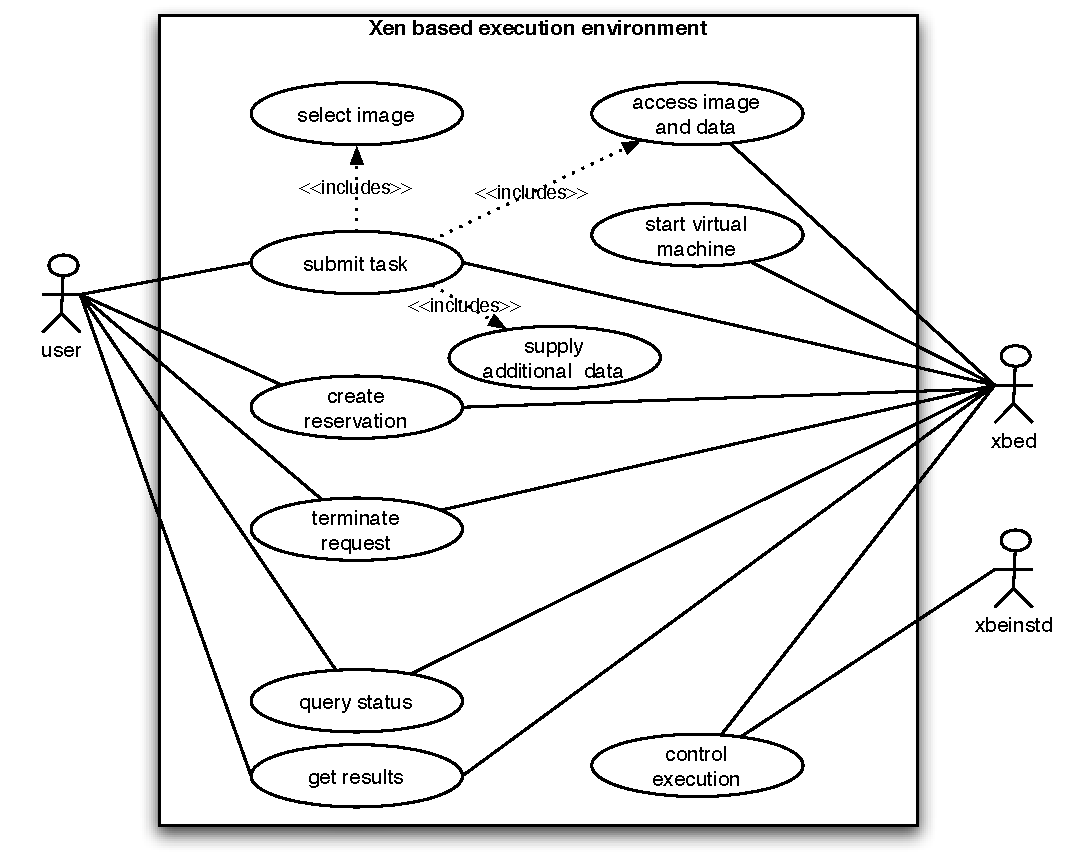
\includegraphics[scale=0.7]{system-usecase}
  \end{center}
  \caption[Use case  overview]{An overview  of several possible  use cases
    and the involved actors.}
  \label{fig:system-usecases}
\end{figure}


\subsection{Task submission}
\label{sec:uc-task-submission}

The very  first use case is  the submission of a  \emph{simple} task. With
\emph{simple} I mean, that the  task does not require any additional data,
it just  requires a previously prepared \gls{glo:image}  that contains the
application and the \emph{xbeinstd}.

On  server-side, the  \emph{xbed}  will associate  the  submission with  a
previously acquired  reservation ---  i.e.~the user creates  a reservation
first  which results in  some kind  of handle  (a unique  identifier which
refers to the  reservation) and then the user submits  his task using that
reservation.

\begin{figure}[htbp]
  \begin{center}
    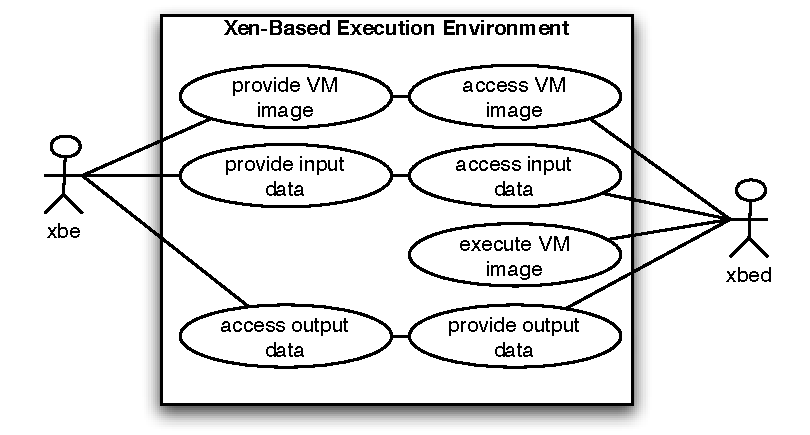
\includegraphics[scale=.75]{uc-submit-task}
  \end{center}
  \caption[UC Task submission]{Actors involved  in the task submission use
    case.}
  \label{fig:uc-submit-task}
\end{figure}

\paragraph{Selecting an image}
In  Figure~\ref{fig:uc-submit-task} the  required steps  for  submitting a
task are  shown. The  submission of  a task includes  the selection  of an
image  that  contains  the  application  the user  wants  to  execute.   A
sophisticated process of image-selection  can be rather complicated, since
it involves matching of available images against a description provided by
the user. Such  selection mechanisms are out of the  scope of this thesis,
but  in  a  later  use  case,  server-side  \emph{caching  of  data}  (see
Section~\ref{sec:uc-data-caching}),  a  simple way  of  selection will  be
described.

\paragraph{Accessing the image}
After the user submitted a  task, the \emph{xbed} has to \emph{access} the
specified image,  i.e.~the \emph{xbed} will initiate the  retrieval of the
image.   The  location  of  the  image  can for  example  be  given  as  a
\gls{glo:URI}  to   provide  an  uniform  and   extensible  mechanism  for
describing data locations.

If errors occur  during the image retrieval, the  \emph{xbed} has to abort
the task execution and must inform the user about the failure.

\subsection{Data staging}
\label{sec:uc-data-staging}

This  use case  is an  enhancements  over the  previous one,  it not  only
involves the  submission of an image,  but also the  specification of data
that  must  be  available  prior  executing  the task  and  that  must  be
transfered back to user after the task has finished.

\begin{figure}[htbp]
  \begin{center}
    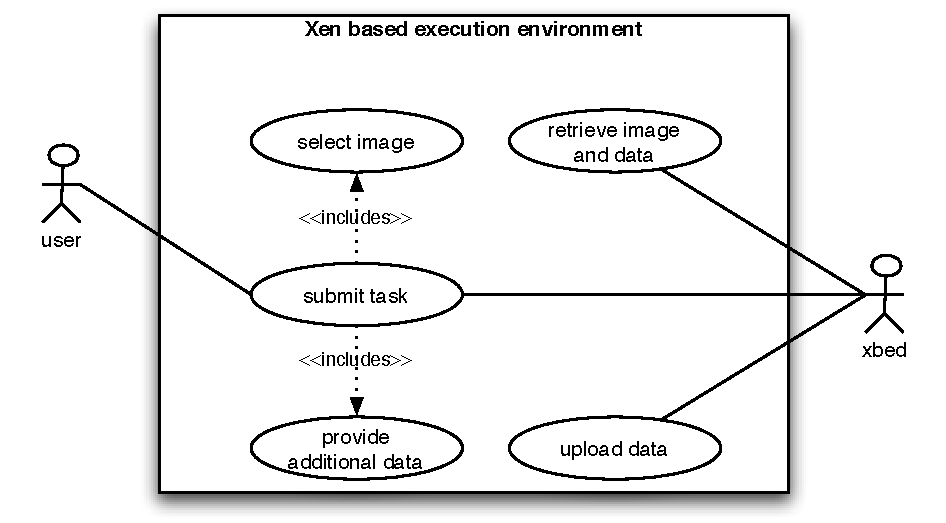
\includegraphics[scale=.75]{uc-data-staging}
  \end{center}
  \caption[UC  Data  Staging]{A user  submitting  a  task with  additional
    data.}
  \label{fig:uc-data-staging}
\end{figure}

Again,  the JSDL comes  into play  here, because  it already  supports the
description of staging operations. The \emph{xbed} has now to retrieve not
only  the image  file, but  also  all the  additional files  the user  has
specified to be staged in.

After the job  has finished its execution, the  \emph{xbed} is responsible
for staging  out generated  files. Therefore the  user must  specify which
files that are and to which locations they have to be uploaded. Source and
destination locations of files can again be specified as \gls{glo:URI}s.

\subsection{On-demand VM-deployment}
\label{sec:uc-on-demand-vm-deployment}

Well, this use  case can be seen  as a variant of the  task submission use
case. The purpose of this use case is the creation of a virtual machine on
user request without executing any task.

The resulting virtual  machine could be accessed by  the user through some
remote mechanism such as \gls{glo:SSH} \cite{openssh}.  With \gls{glo:SSH}
the user gains full control over his created virtual machine and can setup
and install any application he likes.

The login  to the  VM can  be provided using  public-keys that  are either
previously  installed  into the  image  or  uploaded  later on  using  the
standard   stage-in   process  (please   consult   the  documentation   on
\gls{glo:SSH} for more information about public-key authorization).


\subsection{Caching of data}
\label{sec:uc-data-caching}

Imagine a user,  who wants to execute the  same application several times.
That would mean he has to submit the same image over and over again, which
imposes a heavy load on the network connecting user and provider (i.e. the
host on which the \emph{xbed} runs). It would be wise to provide a caching
mechanism, that  allows the  user to store  his image on  server-side. The
caching efficiently  reduces network load and  decreases overall execution
time \cite{locality-principle}.

\begin{figure}[h]
  \begin{center}
    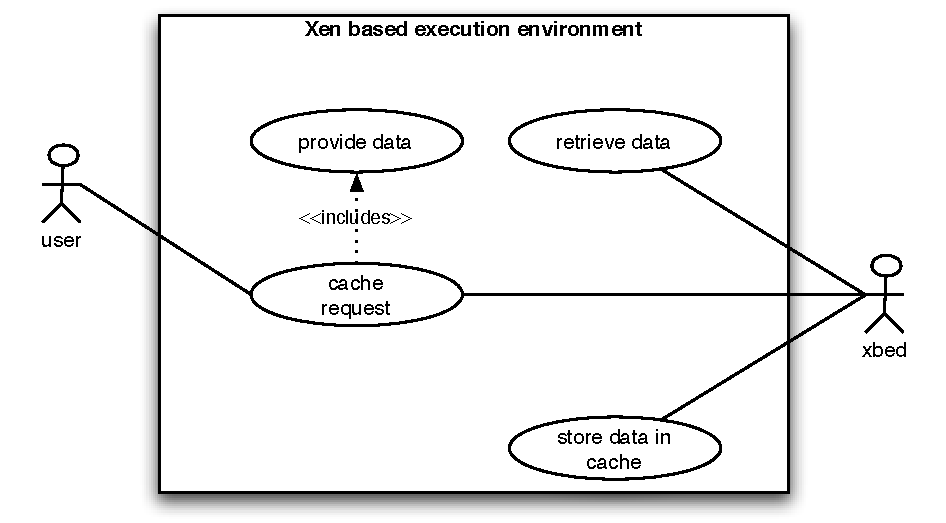
\includegraphics[scale=.75]{uc-data-caching}
  \end{center}
  \caption[UC  Data  Caching]{A user  who  is  requesting  the caching  of
    (arbitrary) data.}
  \label{fig:uc-data-caching}
\end{figure}

In  Figure~\ref{fig:uc-data-caching} the required  steps for  caching some
data are  shown. The user  makes his request  for caching the data  to the
\emph{xbed}, which in turn retrieves the data and stores it in a cache. To
make  the ``discovery''  of cached  data easier  for the  users,  the user
should be required to give some descriptive information for the data he is
going to  cache. As the return of  the request, the user  should receive a
unique identifier or an \gls{glo:URI} for the created entry in the cache.

The details  of how  exactly the caching  works are  highly implementation
specific, the most important point is  how the cached data can be referred
to by users of the system at a later point in time.

\paragraph{Referencing cached  data}

Cached data must be referable by the user for subsequent task submissions.
Since the submission of tasks uses \gls{glo:URI}s to indicate the location
of a  file, an obvious  way is  to use a  \gls{glo:URI} here as  well. The
caching of some data should  therefore result in a \gls{glo:URI}, that the
user can use in his job and staging descriptions.

\begin{figure}[h!]
  \begin{center}
    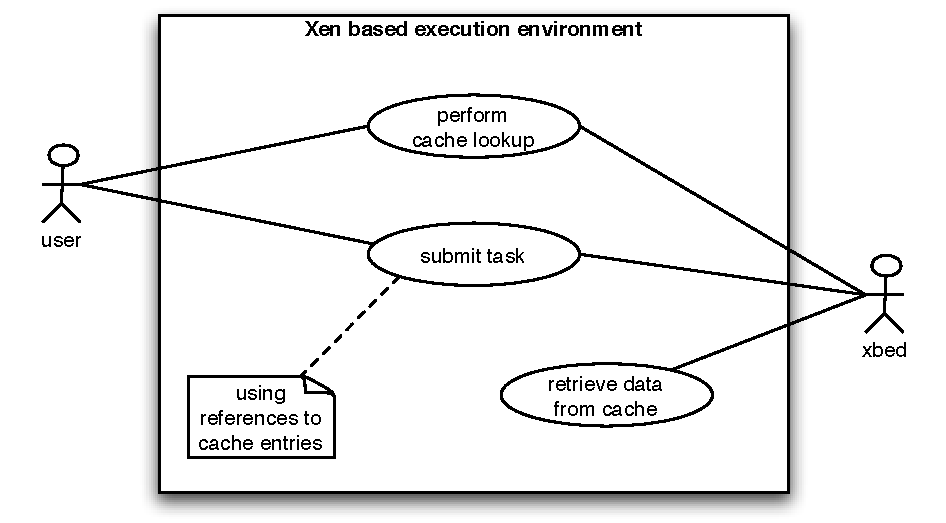
\includegraphics[scale=.75]{uc-cache-lookup}
  \end{center}
  \caption[UC  Cache Lookup]{A user  who  is using cached entries within
    his task submission.}
  \label{fig:uc-cache-lookup}
\end{figure}

Additionally, a really  nice thing to have in this  situation is some kind
of a lookup mechanism for cached  entries --- i.e.~a user does not need to
remember all the  \gls{glo:URI}s his entries have, but can  use a query to
the    system   and   thus    figure   out,    which   cache    entry   to
use. Figure~\ref{fig:uc-cache-lookup} shows you  how a user looks up cache
entries and uses them in a subsequent task submission.

\subsection{Terminating a task}
\label{sec:uc-terminate-task}

As   you   could   see   in   the   \gls{glo:BES}   job   state-model   in
Figure~\ref{fig:bes-extended},  the  user  must  have the  possibility  to
terminate his  submitted task at any  time and no matter  what the current
state of the task is.

\begin{figure}[h!]
  \begin{center}
    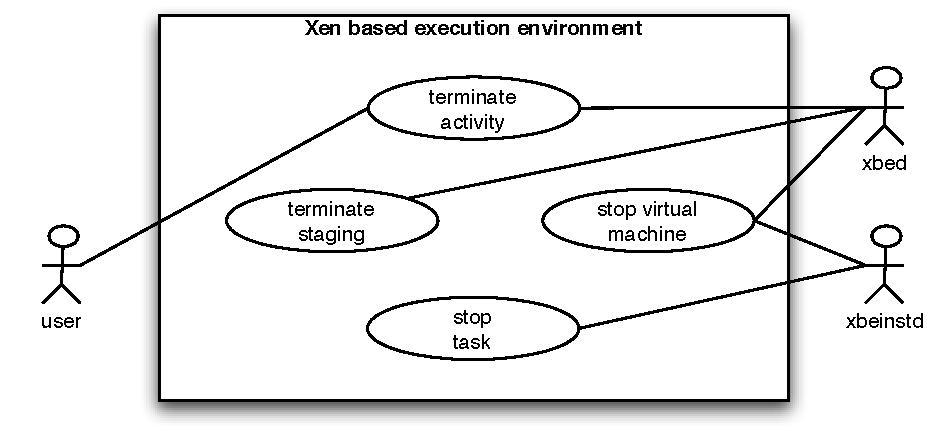
\includegraphics[scale=.75]{uc-terminate-task}
  \end{center}
  \caption[UC Terminate Task]{A user  who is requesting the termination of
    his  submitted task  and possible  use cases  that may  then  arise on
    server-side.}
  \label{fig:uc-terminate-task}
\end{figure}

The termination request  for a task can be received in  any state and that
may require  additional actions to be  taken in the  \emph{xbed}.  If, for
instance,  a virtual  machine has  already been  created and  is currently
executing the user's task, the application and the virtual machine have to
be terminated, too.  The same  holds for staging activities, that could be
currently active, they  have to be terminated cleanly  as well.  These use
cases are  shown in  Figure~\ref{fig:uc-terminate-task}. As you  can seen,
the \emph{xbeinstd} may be involved again, since the actual execution of a
task falls within his responsibility.

\subsection{Providing encrypted data}
\label{sec:uc-ecrypted-data}

Since all  data is referred to  by \gls{glo:URI}s, that  may be accessible
not  only  from  the  \emph{xbed}  itself, but  also  from  other  sources
(i.e.~probably unknown and  hostile ones), it is desirable  to store those
files encrypted. Of  course, if a user stores  an encrypted image-file and
wants  the \emph{xbed} to  use it  for execution,  the image-file  must be
decrypted on server-side prior booting a virtual machine with it.

\begin{figure}[h!]
  \begin{center}
    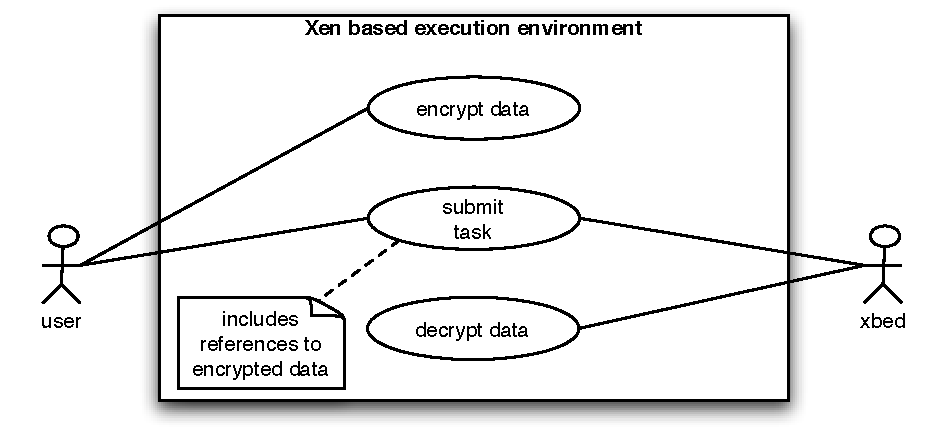
\includegraphics[scale=.75]{uc-encrypted-data}
  \end{center}
  \caption[UC  Encrypted  Data]{Submission   of  encrypted  data  and  its
    decryption prior execution by the \emph{xbed}.}
  \label{fig:uc-terminate-task}
\end{figure}

\section{Security issues}
\label{sec:security-requirements}

The proposed system  will use message queues to  transfer messages between
clients and the server, that means  all messages that are sent can be read
by any person or system in between any two communication partners. 

A   typical  solution   to  make   the  transfer   secure  is   using  the
\emph{Transport Layer  Security} protocol --- or  \gls{glo:TLS} for short.
\gls{glo:TLS} makes sure that  traffic between two endpoints is transfered
securely --- i.e.~no eavesdropping, modification or message forgery.

The  \emph{Transport Layer  Security} protocol,  which is  discussed  in a
moment, and the afterwards examined \emph{Message Layer Security} protocol
are  both using cryptographic  certificates such  as \emph{\gls{glo:X509}}
certificates.

The  certificates  are  based  on  public/private  key  pairs,  whereas  a
certificate consists of a  pair's public-key combined with some additional
information, e.g.~the owner and issuer of the certificate, used algorithms
and  so  on.  Most  importantly  is the  fact,  that  certificates can  be
\emph{cryptographically    signed}     by    a    certificate    authority
(\gls{glo:CA}). The  next passage  will shortly describe  how certificates
can  be  used  in  a  \emph{Public Key  Infrastructure}  using  public-key
cryptography.

\subsection{Public Key Infrastructure (PKI)}

A  \emph{Public Key  Infrastructure} provides  the authentication  of user
identities using certificates.  The main  aspect is that there are special
\textbf{trusted} authorities (\emph{Certificate Authority}, \gls{glo:CA}),
that are permitted  to \textbf{sign} other certificates.  If  a user wants
to prove his  identity to another entity, his  certificate is validated by
that entity, if it is valid, the prove has been successful.

The \gls{glo:CA} is responsible for checking that the public-key contained
in  the certificate  actually belongs  to the  requesting user,  server or
other  entity denoted  in the  certificate. This  checking process  is for
example done by  verifying the credentials of a user  (e.g.~with help of a
photo identification or something similar).

Any third-party that trusts a given CA will transparently trust any entity
that offers a certificate signed by that particular CA.

\begin{figure}[h]
  \begin{center}
    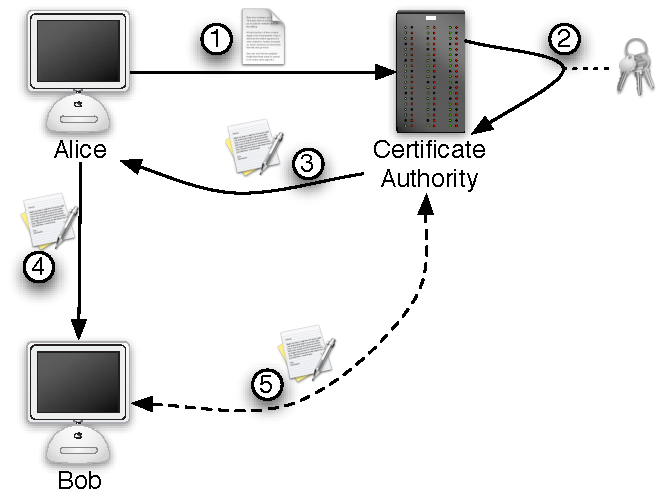
\includegraphics[scale=.75]{pki}
  \end{center}
  \caption[Public  Key Infrastructure]{Alice  proofs her  identity  to Bob
    using a certificate  that is signed by a CA that  both, Alice and Bob,
    trust.}
  \label{fig:pki}
\end{figure}

Validation is performed by verifying  that the certificate itself has been
signed  by a  trusted authority  --- the  actual validation  process  is a
little   bit  more  complex,   since  it   involves  checking   against  a
\emph{Revocation List} and  a ``best before'' date (i.e.~life  time of the
certificate), too.

The  signing  process  uses  the  authority's private  key  to  compute  a
cryptographic signature. This private-key must of course be kept in a very
secure  location  (e.g.~on a  physically  from  the Internet  disconnected
computer) ---  if it would fall into  the wrong hands, the  whole chain of
trust is compromised.

An  example verification  process  is shown  in Figure~\ref{fig:pki},  the
steps can be described as follows:
\begin{enumerate}
\item \emph{Alice} request the signing of her certificate by a CA and thus
  sends a certificate request to the CA containing her public-key.
\item The CA in turn verifies Alice's credentials and eventually signs the
  certificate with its private key.
\item The signed certificate is sent back to \emph{Alice} for her later use.
\item Now,  \emph{Alice} wants to prove  her identity to a  friend of her,
  \emph{Bob},   therefore   \emph{Alice}    sends   her   certificate   to
  \emph{Bob}.  The   proof  may  be   necessary  to  establish   a  secure
  communication over an insecure channel, e.g.~the Internet.
\item \emph{Bob}  verifies the received certificate against  the very same
  CA by  which \emph{Alice} had her certificate  signed.  Since \emph{Bob}
  trusts the  CA and the received  certificate states, that  it belongs to
  his  friend \emph{Alice},  he  can be  assured,  that he  is talking  to
  \emph{Alice}.
\end{enumerate}

\bigskip

Both  of  the following  protocols  can make  use  of  a \gls{glo:PKI}  to
authenticate communication partners.

\subsection{Transport Layer Security (TLS)}

The \gls{glo:TLS}  protocol is often  offered by web- or  email-servers to
make  the  communication   with  a  client  (such  as   a  browser  or  an
email-client) secure.

On-line   banking,   for   instance,   typically   requires   a   Personal
Identification Number  (PIN) to make sure  that it is actually  you who is
trying to access your accounts.  Using unencrypted transfer of the PIN and
other data would mean, that any  system, which is in between your computer
and the  one of your  bank, is  able to read  your PIN and  probably other
information about you. It is also possible that a \emph{man-in-the-middle}
spoofs or modifies  transactions to withdraw money from  your account. Two
things are  very important in  this case: The  first and most  obvious is,
that the information you and  your bank exchange are encrypted. The second
requirement is,  that you  are able  to verify that  the receiver  of your
messages is actually a computer belonging  to your bank and not to someone
else.

\gls{glo:TLS} uses  certificates on the  server-side, so that  clients can
validate  that  they  are  actually  communicating with  the  server  they
intended to  communicate with.  In  the case of  a bank or  any well-known
service  provider   in  the  Internet,  the  certificates   in  place  are
cryptographically  signed by a  \emph{trusted} authority.   A certificate,
that is signed by such an authority you trust, is automatically assumed to
actually belong to the server where the certificate came from.

\bigskip

Unfortunately, \gls{glo:TLS}  cannot be used in a  message-queue system to
secure the traffic  between clients and servers. That  is because there is
no direct connection between client and server --- both are just connected
to their message-queue server. \gls{glo:TLS} can in this case only be used
to secure  the communication between  any end-point and  the message-queue
server it  is connected to.

After transmitting a message over a with \gls{glo:TLS} secured connection,
the  message is  stored in  clear text  on the  message-queue  server. The
message   will  then   again  be   transmitted  securely   to   the  final
destination. But  any person  or system with  access to  the message-queue
server can read, modify or even spoof transmitted messages --- without the
knowledge of either sender or receiver.

To  secure  the  logical   message-based  communication  between  any  two
end-points, a  different kind of security  layer has to be  used here: the
\emph{Message Layer Security} --- or \gls{glo:MLS} for short.

\subsection{Message Layer Security (MLS)}

As the name of this protocol  may already suggest, the security focuses on
the transmitted messages not on  the transportation of the messages.  That
means, the transport layer over which  messages are sent is not altered or
secured in any way  --- it can be as insecure as  before.  But even though
the messages are transmitted over a potentially insecure channel, they are
still protected against eavesdropping, tampering and spoofing.

\gls{glo:MLS} too makes use  of certificates to provide authentication and
encryption. To  establish a  secure communication between  a client  and a
server,  the  client  needs  to  \emph{know}  (i.e.~have  access  to)  the
certificate  of the server.   Since encryption  with a  public/private key
algorithm   is    rather   slow,    in   most   cases    a   \emph{session
  key}\footnote{typically  random data}  will be  negotiated  first.  This
session  key is  then used  to perform  \emph{symmetric} ciphering  of the
messages, which is a lot faster.

\bigskip

The \gls{glo:XenBEE}  must make use  of \gls{glo:MLS} to  provide security
for  its users.   Additionally, as  it is  common  among Grid-middlewares,
\gls{glo:X509}  certificates  are   used  to  authenticate  and  authorize
users. The  server is going  to use a  user's certificate to  validate his
identity and  possibly to send messages  the user --- thus  both sides may
initiate a secure communication.


%%% Local Variables: 
%%% mode: latex
%%% TeX-master: "main.tex"
%%% End: 

\setchapterpreamble[o]{%
  \dictum[Steve Jobs]{\textit{``Design is not  just what it looks like and
      feels like. Design is how it works.''}}}

\chapter{Design and Implementation}
\label{cha:design}

This chapter is about the design and implementation of the \emph{Xen-Based
  Execution  Environment} (\gls{glo:XenBEE}).   The  execution environment
incorporates  a total  of three  main  components: the  \emph{xbe} on  the
user's side, the \emph{xbed} on  the server's side and the \emph{xbeinstd}
on  the  side of  a  single virtual  machine.   All  components have  been
implemented     using    the     \emph{Python}     programming    language
\cite{python-language}. In particular, version  $2.5$ of that language has
been used.

Some additional  modules and programs which  are not part  of the standard
libraries shipped with Python have  been used, though. Among these are for
instance  the \texttt{twisted}  framework \cite{twisted-python}  which has
been  used  for  the  network  code,  a  library  called  \texttt{libvirt}
\cite{libvirt}  that  was used  to  connect  to  the Xen  virtual  machine
monitor, and a library that  provides Python bindings to the \texttt{curl}
library \cite{pycurl}.


\section{Overview}
\label{sec:design:overview}

The picture in Figure~\ref{fig:architecture-overview} shows an overview of
the three components which, when put together, make up the \emph{Xen-Based
  Execution  Environment} (\gls{glo:XenBEE}).

\begin{figure}[ht]
  \centering
  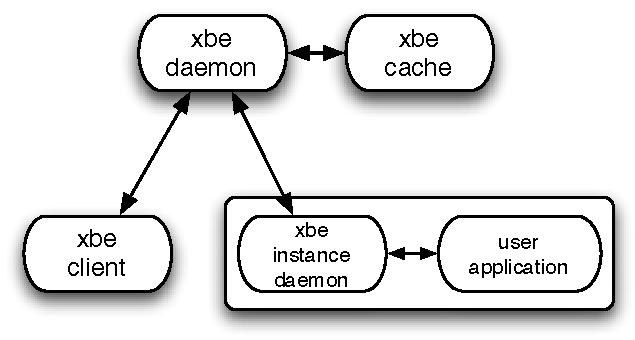
\includegraphics[scale=.7]{architecture-overview}
  \caption[Overview of the  \gls{glo:XenBEE} components]{The components of
    the Xen-Based Execution Environment}
  \label{fig:architecture-overview}
\end{figure}

The ``thicker'' connections between \emph{xbe} and \emph{xbed}, as well as
between \emph{xbed}  and \emph{xbeinstd} are  logical connections realized
by using message-queues and one or more \gls{glo:MQS} in between.  Whereas
the ``thinner'' links are either inner-process connections (in case of the
cache) or  connections between  parent and child  process (in case  of the
user-application).

On the left hand side of the picture are the users using the \emph{xbe} to
communicate with the execution  environment. The \emph{xbe} refers in this
case  to the command  line tool  which I  have implemented  as a  proof of
concept  to interact  with the  \emph{xbed}.  The  interface that  an user
utilizes to execute his applications  with the \gls{glo:XenBEE} could be a
web-portal or some other tool with a graphical user interface as well.

\medskip

On the right hand side are the components that are required to execute the
applications within  virtual machines.  The \emph{xbed} has  to be running
on a machine  that supports the Xen hypervisor.   It maintains an internal
connection  to a local  cache which  can be  used by  any user  to deposit
arbitrary data on the  server side.  The \emph{xbed} uses \texttt{libvirt}
to connect to the Xen hypervisor and to manage active virtual machines.

Each  virtual machine  must  provide  the \emph{xbeinstd}.  It  has to  be
started  at some  point during  the  initialization process  of the  guest
operating system. Any image that is submitted to the execution environment
must therefore  contain this  program. The \emph{xbeinstd}  is responsible
for two  major issues:  executing the actual  application and  keeping the
virtual machine instance alive.   Execution of an application involves for
instance  passing  arguments  to   the  executable,  setting  the  working
directory and redirecting the input and output streams. The \emph{xbed} is
going  to shut  stale virtual  machines down,  unless  the \emph{xbeinstd}
sends  regular keep-alive  messages  to the  \emph{xbed}.   If the  user's
application has finished, the \emph{xbeinstd} signals the \emph{xbed} that
the virtual machine is ready to be shut down.

\section[The Xen-Based Execution Daemon]{The Xen-Based Execution Daemon (xbed)}
\label{sec:xbed}

This  section describes  the  ``heart'' of  the  \gls{glo:XenBEE} ---  the
\emph{xbed}.   The  \emph{xbed}  is  itself composed  of  several  smaller
components that  are each responsible for  a single detail  of the daemon.
The   main   components   though   are   the   \texttt{TaskManager},   the
\texttt{InstanceManager} and  the \texttt{Cache}.  The latter  is a rather
simple implementation of  a local data cache which will  be discussed in a
later section.

\begin{figure}[ht]
  \centering
  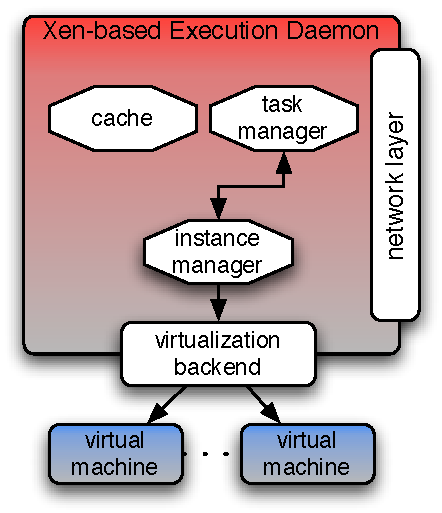
\includegraphics[scale=.55]{xbed-architecture}
  \caption[Components of the xbed]{The most important components of the xbed}
  \label{fig:xbed-architecture}
\end{figure}

\subsubsection{Network Layer}

On startup, the  daemon tries to connect to  the message-queue server that
has been  defined either in  its configuration file  or as a  command line
parameter. This process  is realized by the \emph{network  layer}. It uses
the  \texttt{twisted} framework to  establish a  \gls{glo:TCP} connection.
When the connection has been successfully established, a special transport
protocol  --- the  STOMP  protocol  \cite{stomp} ---  is  attached to  the
connection. STOMP is the \emph{Streaming Text Oriented Messaging Protocol}
and  basically defines a  very simple  protocol to  send and  receive text
messages over a  message-queue server.  On top of  this text message based
protocol are  XML based protocols that accomplish  the whole communication
between  all components.   There is  currently a  basic XML  protocol that
encapsulates single ``messages'', consisting  just of header and body, and
two  protocols  that connect  up  the  \emph{xbe}  and the  \emph{xbeinst}
accordingly.  A special protocol  providing security related services (\ie
privacy and validity) can be added as an additional layer.

Anyway, the details  of the \gls{glo:STOMP} and XML  protocols, as well as
the network  layer which is to  some extent equal among  all components of
the        \gls{glo:XenBEE},       will       be        discussed       in
Section~\ref{sec:communication-protocol},
\emph{\nameref{sec:communication-protocol}}.

\subsubsection{Task-Manager}

When an  user submits,  terminates or  requests the status  of one  of her
jobs, the  message is actually handled by  the \texttt{TaskManager}.  This
component controls all tasks, the system knows of. A ``task'' does in this
case  not refer  to the  actual application  an user  submitted, but  to a
container that holds the task's  state machine, description and probably a
reference to the virtual machine instance used for this task.

A new task gets initialized every  time an user requests a reservation. At
this time it contains nothing more  than the state machine which is in its
start-state                               (\ie \texttt{Pending:Reserved}).
Section~\ref{sec:xbed:job-model}  discusses   the  implementation  of  the
job-model that has been used to  represent an activity.

Each task and each reservation has its own unique identifier by which they
are known  to the system  and to the  user.  Those unique  identifiers are
implemented     by    using     \emph{Universal     Unique    Identifiers}
(\gls{glo:UUID}s).  Whereas  the task identifier is more  or less publicly
available\footnote{a listing  of all current tasks comparable  to the UNIX
  \texttt{ps}  command could be  possible}, the  identifier of  the user's
reservation is  only known to  that particular user (or  some intermediary
software such as  a Calana-agent). All requests that an  user makes to the
system require the reservation's unique identifier.

When an user confirms a reservation,  he also sends the job description as
a \gls{glo:JSDL}  document along with the confirmation  message.  The task
is  thus completely  specified and  may  perform the  transition into  the
\texttt{Executing} state. To this time, the task-manager creates a special
spool directory  for that  task which is  eventually going to  contain all
necessary  files to  create the  virtual  machine and  execute the  user's
application. The  details of how the  required files are  obtained will be
discussed  in   a  later  section  (Section~\ref{sec:xbed:data-transfer}).
After  all   files  have  been   retrieved,  the  \texttt{InstanceManager}
component is used to create a new virtual machine for the task.

\subsubsection{Instance-Manager}

The instance-manager's purpose is  to create, control, monitor and destroy
active virtual  machine instances.  Again  unique identifiers are  used to
name the  virtual machines. To start  a virtual machine  several files are
required:

\begin{itemize}
\item  An  operating  system  installation  which  resides  in  a  special
  file-system \gls{glo:image} file.
\item  A  \gls{glo:kernel}  and   potentially  an  initial  ramdisk  image
  (initrd). The  initrd typically  contains additional device  drivers and
  setup routines that are not directly included in the kernel.
\end{itemize}

These files must  be provided by the user, because she  knows best how the
operating system must be set up to run the specific application.

By just using these three files, a virtual machine cannot be created right
away, it must be \emph{configured}  first.  The configuration of a virtual
machine is manifold, it contains descriptions of the operating system that
is to  be used (\ie the  mentioned three files), memory  settings (\ie the
amount of  virtualized physical  memory), the number  of virtual  CPUs and
network parameters.

\subparagraph{Instance Configuration and Setup}

The \emph{xbed}  provides the possibility to  use different virtualization
back-ends,  but  the  current  implementation supports  only  Xen  virtual
machines. It could, for instance, be possible to implement a back-end that
uses VMWare's  \cite{vmware} virtual machines, even no  virtual machine at
all could be thinkable.

The back-end uses  the \texttt{libvirt} \gls{glo:API} to connect
to  the Xen hypervisor.  This connection  is basically  used to  query the
current state of  a virtual machine and to shut  a running virtual machine
down.   Virtual machine creation  is implemented  by using  a call  to the
\texttt{xm} command line tool provided by the Xen user-space tools.  Prior
a  new  instance   can  be  created,  a  configuration   file  has  to  be
generated. This configuration file contains the mentioned parameters.

The  network  configuration   of  a  virtual  machine  is   based  on  the
\emph{Dynamic Host Configuration  Protocol} (\gls{glo:DHCP}).  That means,
the guest  \gls{glo:OS} has  to be configured  to use  \gls{glo:DHCP}. The
administrator of  the host, on which  the \emph{xbed} runs,  can specify a
list  of  \gls{glo:MAC}  addresses  that  shall be  used  by  the  virtual
machines. In addition to  these \gls{glo:MAC} addresses, the administrator
can also  specify a \gls{glo:URI}  or an IP  address by which  the virtual
machine

Virtualized  physical  memory  and  the  number of  virtual  CPUs  can  be
specified  in the  \gls{glo:JSDL} document  using the  predefined resource
descriptions.

\subparagraph{Instance Creation}

The next step is the generation  of a configuration file which can be used
by the back-end --- in this case  Xen --- to set up a new virtual machine.
The task's  state machine  is triggered  to change its  state to  the next
sub-state   of  \texttt{Running}:  \texttt{InstanceStarting}.    Once  the
virtual machine has  been created, the \emph{xbed} awaits  a callback from
the virtual machine.  This callback  expresses itself in form of a message
sent  by  the \emph{xbeinstd}  running  within  the  just created  virtual
machine.  If  this signal does  not get sent  within a given  timeout, the
virtual machine  instance is  assumed to be  broken. The  \emph{xbed} will
therefore shutdown  and destroy  this virtual machine.   Consequently, the
execution  of the  user's task  has  failed.

The callback  from the  \emph{xbeinstd} fulfills two  important functions.
Firstly it makes sure that  the virtual machine's network configuration is
correct  and   fully  functional.   Secondly  it  is   verified  that  the
\emph{xbeinstd}  is  installed  in  the  image  and  did  start  properly.
Improperly configured images are thus recognized very fast.

Now, that the virtual machine  is ready to execute the user's application,
the task's description  may be sent to the  \emph{xbeinstd} and the task's
state machine  may eventually change its state  to \texttt{Executing}. The
details  of  executing  the  application  is  going  to  be  discussed  in
Section~\ref{sec:xbeinstd}.

After  finishing the  execution  of the  user's  application, the  virtual
machine will  be shut down and the  result can be staged  out according to
the specified \gls{glo:JSDL} document.

The next sections  describe the implementation of the  used job-model, how
the staging  of input  and output data  is performed  and how an  user can
benefit from using the provided data-cache.

\subsection{Job-model Implementation}
\label{sec:xbed:job-model}

In     the     sections    \emph{`\nameref{sec:fundamentals:bes}'}     and
\emph{`\nameref{sec:calana-support}'}               on               pages
\pageref{sec:fundamentals:bes}       and      \pageref{sec:calana-support}
respectively, I have already discussed the usage of the job-model that has
been  proposed  by the  \gls{glo:OGSA}-\gls{glo:BES}  working group.   The
Calana  architecture   requires  the  model  to   contain  extensions  for
\emph{reservation} and \emph{data staging}.

To model  the process of starting  a virtual machine, I  have extended the
model  again  to provide  an  additional state  \texttt{Instance-Starting}
which  is a  sub-state  of  the basic  state  \texttt{Running}. The  final
job-model is shown in Figure~\ref{fig:bes-job-model}.

\begin{figure}[ht]
  \centering
  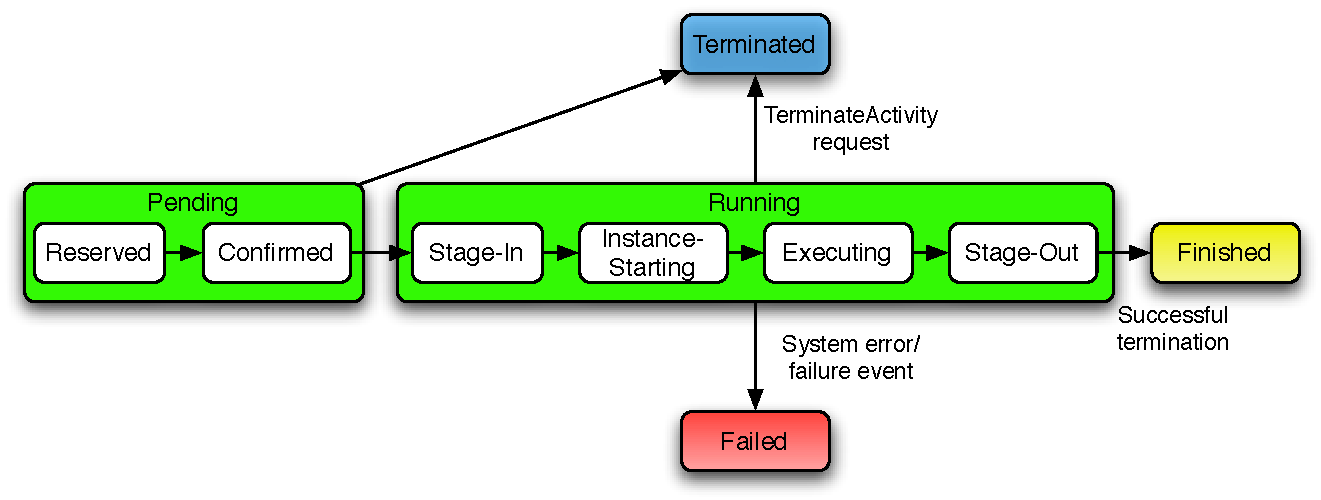
\includegraphics[scale=.55]{bes-job-model}
  \caption{The job-model used in the \gls{glo:XenBEE}}
  \label{fig:bes-job-model}
\end{figure}

The  implementation of  this model  builds up  on an  implementation  of a
\emph{Finite  State  Machine}  (\gls{glo:FSM}).  The  \texttt{Task}  class
contains a reference to an instance  of such an \gls{glo:FSM}. Each time a
state  change is  desired the  \gls{glo:FSM} is  called with  an ``input''
signal. The  \gls{glo:FSM} then calls registered  functions that implement
the transition's behavior. If, for example, an user wants to terminate his
activity, the  \gls{glo:FSM} is presented with  a ``terminate-token''. The
FSM  calls  then specialized  functions  that  deal  with the  termination
request according to the current state. That means, distinct functions are
perhaps   called  when   traversing  from   \texttt{Pending:Reserved}  and
\texttt{Running:Executing} to the \texttt{Terminated} state, respectively.

Some of the transitions  involve rather complex and time-consuming actions
(\eg  file  transfers).   Those  complex transitions  are  represented  by
\emph{activity-objects}.    An   activity-object   is  an   object   which
encapsulates  some behavior  along  with  a state  ---  commonly known  as
\emph{Function}-objects or \emph{Functors}.  I named them activity-objects
on  purpose, because they  are usually  executed by  a separate  thread of
control  in concurrency  to other  activities within  the  system. Another
reason for  encapsulating some of  the transitions in  activity-objects is
the possible intervention by an user.

The  BES model  allows an  user to  terminate his  task at  any  time.  In
particular  that means,  that any  action  belonging to  that task,  which
currently takes place on the server, has to be stopped or aborted.

Since the task-manager does not only create, but also manage the tasks, he
is responsible  for stopping current activity-objects  of a task  if he is
asked to do so.  For that reason, he  is in charge of a per task list that
contains all  current activity-objects for that task.  If the task-manager
is now going to  handle a request for termination of one  of the tasks, he
first cancels  all registered activity-objects before letting  the task to
change its state to \texttt{Terminated}.

\begin{figure}[ht]
  \centering
  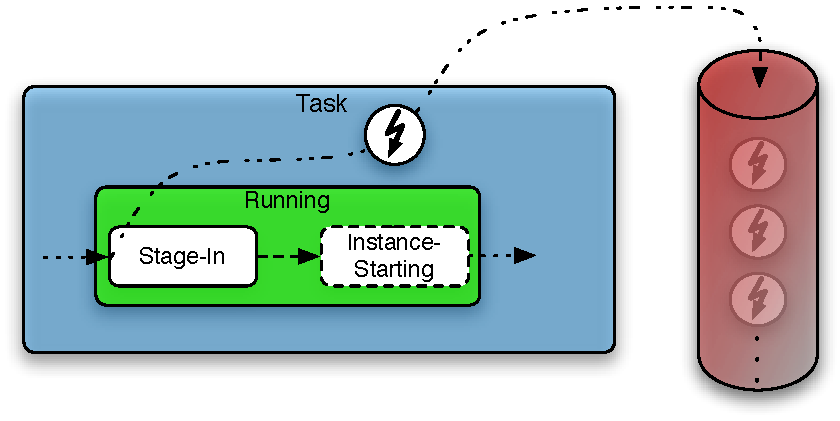
\includegraphics[scale=.55]{activity-queue}
  \caption{Handling of \emph{activity-objects} with an activity-queue.}
  \label{fig:activity-queue}
\end{figure}

The picture in Figure~\ref{fig:activity-queue} shows such a case. The task
(represented  by  the blue  box)  is  currently  in the  \texttt{Stage-In}
sub-state  of \texttt{Running}  and is  awaiting the  availability  of its
required files.   The activity-object which represents  here the operation
of staging  files in is shown  as the encircled lightning  bolt.  When the
task transitions into the  \texttt{Stage-In} state, it registers the shown
activity-object with the task-manager. The task-manager in turn adds it to
his queue  of current activity-objects (shown  as the reddish  tube in the
right of the picture).  When the activity-object is finished (figuratively
speaking: if the lightning bolt exits through the bottom of the tube), the
task may  advance its state  to \texttt{Instance-Starting}, \ie it  can be
attempted to start an instance for this task.

Since  the  retrieval of  files  from  different  locations (specified  by
\gls{glo:URI}s  in the \gls{glo:JSDL})  may take  some time,  this example
also motivates  the usage of threads  to decouple other  activities of the
system from these steps.  When terminating a threaded activity-object, the
responsible thread is signalled to abort whatever it is doing at the time.

The  whole   cycle  through   which  a  task   may  run  is   depicted  in
Figure~\ref{fig:act-execute-task}  on  page~\pageref{fig:act-execute-task}
as an activity  diagram.  The only sub-activity that  cannot be aborted at
all is  the \emph{stop instance}  operation. That is because  the shutdown
process  of the  underlying virtual  machine just  cannot be  cancelled or
reversed. That  is also the  reason to not  having an extra  sub-state for
that operation in the job-model.

\begin{figure}[ht]
  \centering
  \includegraphics[scale=.55]{act-execute-task}
  \caption[Summary of executing a task]{Summary of the steps involved when executing a task.}
  \label{fig:act-execute-task}
\end{figure}

The  process starts  with waiting  on  a ``ready-to-go''  signal which  is
usually included  directly in the \texttt{Confirm} message  received by an
user,  but  can  also  be  given  in  a  subsequent  message  on  its  own
(\texttt{Start\-Request})\footnote{the  communication   protocol  and  the
  messages           involved          are           discussed          in
  Section~\ref{sec:communication-protocol},
  \emph{\nameref{sec:communication-protocol}}.}.  The  next steps resemble
the  previously discussed  job-model. Of  course, any  of those  steps may
\emph{fail}, which effectively  results in the failing of  the whole task.
The operations that are involved  when one of the sub-activities fails are
the  same  as  for  the  abortion of  that  sub-activity.   Actually,  the
\emph{stop instance} operation cannot fail, since it is always possible to
forcibly shut down a virtual machine.

The \emph{start  instance} operation differs from the  other operations in
that two components are involved, the \emph{xbed} and the \emph{xbeinstd}.
The \emph{xbed}  first attempts  to start a  back-end instance (\eg  a Xen
virtual machine) and waits for the instance to be started, eventually.

After the instance  has been started, \ie the back-end  did not reject the
provided  configuration, the  \emph{xbed} (actually  the  thread executing
this particular activity-object) waits  for the \emph{xbeinstd} to send an
\texttt{Instance\-Available}        message       back        to       the
\emph{xbed}. Figure~\ref{fig:act-start-instance} shows the details of that
particular step.

\begin{figure}[ht]
  \centering
  \includegraphics[scale=.55]{act-start-instance}
  \caption[Start Instance Activity]{The  \emph{xbed} waits for the virtual
    machine to  be available.   The availability of  a virtual  machine is
    made sure by waiting on a special message from the \emph{xbeinstd}.}
  \label{fig:act-start-instance}
\end{figure}

As you  can see,  there are  three different outcomes  for this  step. The
instance  can  be  marked  as  being  available  which  renders  the  task
eventually executable,  the step can as  well be aborted due  to a request
for termination by the user or the  instance can fail to start at all. The
task's state will be changed according to the outcome of this step.

After   sending   the   \texttt{Instance\-Alive}   notification   to   the
\emph{xbed},  the  \emph{xbeinstd}   waits  for  the  task's  description.
Additionally,  it will send  messages to  the \emph{xbed}  regularly, thus
making sure, that the virtual machine is still ``alive''.

The  next section deals  with the  staging operations  in more  detail. In
particular this means, how exactly  the files are retrieved, how files can
be compressed  to reduce  the required network-bandwidth  and how  one can
make sure that the files have been transferred correctly.

\subsection{Data Transfer Handling}
\label{sec:xbed:data-transfer}

The  handling  of data  transfer  covers the  staging  of  files into  the
execution environment and out from the execution environment, in this work
referred   to  as  ``stage-in''   and  ``stage-out''   respectively.   The
description  that  is  required  for  each of  the  staging  processes  is
completely  covered  within  the  \gls{glo:JSDL} document  which  an  user
submitted  to the  execution  environment.  However,  some extensions  are
required,       those       will       be      handled       with       in
Section~\ref{sec:xen-based-submission}.

The  stage-in process  is  twofold.  The  first  part of  stage-in is  the
acquirement of files  that are mandatory for the  execution environment to
create    virtual    machine,    these    are    the    early    mentioned
\emph{\gls{glo:image}}  and  \emph{\gls{glo:kernel}}  files  (probably  an
\emph{\gls{glo:initrd}}  as well).   Without  these files,  the next  part
cannot be started.

The second  part of the stage-in  process handles the input  files that an
user had specified for his application. These definitions use the standard
\texttt{DataStaging}  element of  the \gls{glo:JSDL}  specification. These
files  are directly  retrieved into  the virtual  machine image  which was
previously obtained, hence the two parts of the staging process.

All files, including the virtual machine specific ones, are referred to as
\emph{Uniform  Resource  Identifier}s  (\gls{glo:URI}s). That  means,  all
files must be ``somehow'' accessible by the \emph{xbed}.  An user can, for
instance, specify files that  are located on an \texttt{\gls{glo:HTTP}} or
on an \texttt{\gls{glo:FTP}} server --- currently only these two protocols
and  a special  URI to  reference to  cached files  are  supported.  Those
\gls{glo:URI}s are then retrieved by the \emph{xbed} by using the standard
mechanisms for  file retrieval  based on these  protocols ---  the library
\texttt{libcurl}, which relates to the UNIX \texttt{curl} command, is used
to implement download and upload.

\subsubsection{Support for compressed files}

As said before,  all input files related to  the application are retrieved
into  the virtual  machine image  directly. Consequently,  the  image must
provide enough  free space  to hold all  input and generated  output data,
which  can be  quite a  lot. Since  the  image is  an ordinary  file on  a
file-system, it can  easily consume unpredictable size. This  image has to
be  transfered  from  the user  (\ie  the  location  he specified  in  the
\gls{glo:JSDL}) to  the host on  which the \emph{xbed}  runs. Fortunately,
the image is nearly empty before transmitting it, since it contains only a
basic operating system installation  along with the user's application and
its dependencies.

The \emph{xbed} allows an user to submit compressed files. The compression
is extremely  useful when the file is  mostly ``empty'' as it  is the case
for the  image files, for  instance --- an  image file that was  $8$~GB in
size and contained  about $750$~MB data produced a  compressed file (using
\texttt{bzip2})  that was  about  $500$~MB  in size  only.   The usage  of
compressed files  reduces the  time needed to  transfer large,  but mostly
empty images significantly. The user is allowed to tag every file that she
submits to the execution environment  with the mode of compression and the
\emph{xbed} will decompress the file after retrieval.

\begin{figure}[ht]
  \centering
  \includegraphics[scale=.55]{act-retrieve-file}
  \caption[File  Retrieval  Activity]{Steps  involved when  retrieving  a
    \gls{glo:URI}.}
  \label{fig:act-retrieve-file}
\end{figure}

\subsubsection{Support for validation of files}

Figure~\ref{fig:act-retrieve-file} shows the involved steps when a file is
retrieved by the \emph{xbed}. Another feature added to this process is the
validation of the retrieved data. If  an user wants to make sure, that the
file had not been modified in some way, she can provide a checksum and the
used    algorithm   along   with    the   \gls{glo:URI}.     Typically   a
\emph{cryptographic  hash   function}  is   used  to  compute   a  digital
fingerprint of the  data. All secure hash algorithms  that are provided by
the  Python  \texttt{hashlib} module  are  supported  (some examples  are:
\texttt{SHA1}, \texttt{SHA256} or \texttt{MD5}).

\subsubsection{The whole stage-in process}

The  stage-in   process  is   split  into  several   steps  as   shown  in
Figure~\ref{fig:act-stage-in}. The process always starts with the creation
of a \texttt{\gls{glo:chroot}} environment\footnote{The terms \emph{chroot
    environment} and \emph{jail  environment} are used interchangeably.  A
  short description of  a \texttt{chroot} environment can be  found in the
  glossary.}  within  the spool directory  that has been created  for that
task.  The  description of  the necessary files  for a virtual  machine is
contained   in  an   extra  element   within  the   task's  \gls{glo:JSDL}
description. An user can either  specify the required files (image, kernel
and initrd) on  its own or he can specify  a \texttt{bzip2} compressed tar
archive (``package'')  that contains  these files.  Additionally,  an user
has the possibility to define several executable scripts that are uploaded
to  the execution  environment and  get called  at various  stages  of the
stage-in process.

After  the package  or  the  virtual machine  files  have been  retrieved,
validated and  probably decompressed, the ``pre-setup''  hook is executed.
This  hook consists  of the  scripts that  were either  in the  package or
specified  by the user  and tagged  to be  in this  hook. All  scripts are
executed in the previously created \gls{glo:chrootenv} so that they cannot
access any file that does not belong to this task. Until now the execution
environment had  not touched the  image file, so  that one of  the scripts
could be used to decrypt the file, for instance.

\begin{figure}[ht]
  \centering
  \includegraphics[scale=.55]{act-stage-in}
  \caption[Stage-In  Activity]{Overview  of  the  parts  of  the  stage-in
    activity.}
  \label{fig:act-stage-in}
\end{figure}

Now that all virtual machine specific files are available, the application
specific data can be retrieved. The \emph{xbed} assumes, that the image is
mountable by the UNIX \texttt{mount}  command and mounts it to a temporary
location within the jail environment.

All  JSDL-\texttt{DataStaging} elements that  define a  stage-in operation
are now handled with the  same retrieval mechanism as described above. The
paths that are used in the  job description are interpreted to be relative
to the mount point of the image.

Finally   the   ``setup''-hook  is   executed   using  the   user-supplied
scripts. These scripts  are given the path to  the image's mount-point and
can,  for  example,  decrypt  already  staged-in files  or  even  retrieve
additional input  data. If  everything went well,  the virtual  machine is
completely set up and can be started.

\subsubsection{Upload of files}

The upload of files from the execution environment to a location specified
by the user  is also accomplished by using  \gls{glo:URI}s. The process of
uploading a file is less  complicated than the retrieval process, since it
currently does  not involve compression or validation  directly.

The first step  after the virtual machine has been shut  down is again the
mounting of the image to a temporary location within the jail environment.
To provide  the possibility to  compress the files before  uploading them,
the ``cleanup'' hook is called before any of the actual staging operations
is called. The next step  is the handling of the JSDL-\texttt{DataStaging}
elements that  define a stage-out operation. The  only currently supported
protocols that can  be used for the upload  are \texttt{\gls{glo:FTP}} and
\texttt{\gls{glo:HTTP}}.  In the  final  step of  the  upload process  the
``post-cleanup''  hook is  called;  to that  time,  all specified  staging
operations have already been successfully performed and the image has been
unmounted.

If everything  went well, all  stored data\footnote{this does  not include
  internal data structures (\eg exit-code).}  that belongs to this task is
destroyed (\ie  the spool directory will  be deleted) and the  task is put
into the \texttt{Finished} state.

\subsection{Caching Of Arbitrary Files}
\label{sec:caching}

Compression   of  files   can   decrease  the   deployment  time   already
significantly, but  to avoid  long-distance transfers over  an unspecified
network connection, the  caching of files on the  server side is required,
this    follows    strictly    from    the    \emph{locality    principle}
\cite{locality-principle}.  The \emph{xbed} supports this by providing the
user with a  simple data-cache incorporated into the  system.  The user is
able to store  arbitrary data on the server prior submitting  a job to the
system. This makes the initialization  of a virtual machine for often used
images a lot faster compared  to always retrieving them over a potentially
slow network connection.

\subsubsection{Adding data to the cache}

An  user  adds  files  to   the  execution  environment  by  specifying  a
\gls{glo:URI} that can be retrieved by the \emph{xbed}.  This will usually
be the same \gls{glo:URI} the user would have given in his job description
(\eg a location  on some \texttt{\gls{glo:FTP}} or \texttt{\gls{glo:HTTP}}
server).  The \emph{xbed} attempts to retrieve the given \gls{glo:URI} and
adds a new entry to a database.

Actually the  complete mechanism  of caching is  implemented in  a special
component  within  the  \emph{xbed}  on   its  own.   The  cache  uses  an
\gls{glo:SQL}-database  to store information  about the  cached data  in a
persistent way. An user can add two different pieces of information to the
data he wants to have cached.  The first is the \textbf{type} of the data,
which can  be one  of \texttt{image}, \texttt{kernel},  \texttt{initrd} or
\texttt{data},  where the  \texttt{data} type  is just  a  placeholder for
arbitrary data  that does not fit  into one of the  other categories.  The
second piece of information is  a \textbf{description} that can be used to
describe the data in more detail,  \eg the version of a specific kernel, a
list of the applications that are installed within an image or the type of
compression   if  the   data   had  been   compressed.   Additionally   an
\texttt{SHA1}  digital fingerprint  of the  data is  computed  and stored,
along with the provided information, in the database.

The  cache-component  assigns each  entry  a  unique  identifier based  on
\gls{glo:UUID}s, this identifier  can later be used in  a \gls{glo:URI} to
refer to that  entry.  When using the \emph{xbe} command  line tool to add
data to  the cache, the \gls{glo:URI}  of the newly created  entry will be
printed on the screen upon success.

\subsubsection{Discovering cache entries}

The first way of ``discovering'' an  entry of the cache is simply to write
down the  \gls{glo:URI} one has received  upon addition of  the entry. But
that is not always feasible, since the entry could be shared among several
users who do not know each  other --- say, an administrator or provider of
a virtual machine image  added it to the cache, so that  it can be used by
several, to that time unknown, users.

The  discovery of  cached entries  is  implemented in  the \emph{xbed}  by
simply providing the  user with a list of all  entries. This list contains
most importantly the \gls{glo:URI} of the  entry, the type of data and the
description the submitter had given.

\begin{figure}[ht]
  \centering
  \includegraphics[scale=.55]{msc-list-cache}
  \caption[MSC List Cache Entries]{TODO: fill me in}
  \label{fig:msc-list-cache}
\end{figure}

The      \emph{Message     Sequence     Chart}      (\gls{glo:MSC})     in
Figure~\ref{fig:msc-list-cache} shows  the messages that  are sent between
the  client and  the server.   The client  requests a  list of  all cached
entries  by sending  the \texttt{ListCache}  message. Thereupon  makes the
\emph{xbed} a call to the cache-component  that provides him a list of all
entries. This list is eventually  transformed into an XML-message and sent
back to the client.  A sample output of the \texttt{xbe showcache} command
is shown in the following listing:

\bigskip

\begin{center}
  \begin{minipage}{.75\textwidth}
    \begin{lstlisting}[captionpos=b,backgroundcolor=\color{listingcolor},frame=lines,numbers=left,numberstyle=\tiny,caption={\emph{xbe} output of cache entries.},label={lst:xbe-listcache-out}]
<CacheEntries with 1 entry:
{'cache://xbe-file-cache/adfd0a99-4761-4816-8902-db8d62c8e482':
  {'description': 'Ubuntu kernel (2.6)',
   'hash': '732ca16f330c2c382e83cb997f5e027687a285aa',
   'type': 'kernel'}}
>
    \end{lstlisting}
  \end{minipage}
\end{center}

\subsubsection{Using cache entries}

Cache  entries can  be used  rather  easy. The  user is  just required  to
specify  the  \gls{glo:URI} of  a  cache  entry  instead of  the  original
\gls{glo:URI}.   The \emph{xbed} will  lookup the  specified \gls{glo:URI}
during the  stage-in process and  retrieve the data  from the cache,  if a
valid entry  could be found. The  same retrieval mechanism  applies to the
cached entries, so that compression  and validation can be used with them,
too.


\subsection[The Xen-based Submission Description Language]{The Xen-based Submission Description Language (XSDL)}
\label{sec:xen-based-submission}

This  section  describes  the   extensions  to  the  \emph{Job  Submission
  Description  Language} that  were developed.   The extensions  have been
required,  since   the  \gls{glo:JSDL}  does  not   directly  support  the
description of virtual machines.

There are actually two  different kinds of extensions: general extensions,
that  can also  be used  to enhance  some of  the  standard \gls{glo:JSDL}
elements, as well as an extension  that is purely specific to the proposed
execution environment.

\subsubsection{General extension elements}

As  described  above,  the  \gls{glo:XenBEE} supports  the  submission  of
compressed  files and  the  validation  of those  files  based on  digital
fingerprints.   To reflect this  behavior along  with the  job submission,
additional ``decorator'' elements have  been added.  The following example
(Listing~\ref{lst:xbe-xsdl-example}) shows the  usage of these decorators.
The  \gls{glo:JSDL} does only  support plain  \gls{glo:URI}s.  If  such an
\gls{glo:URI} is now used along with  one or more of these decorators, the
\emph{xbed} interprets the URI correctly.

\medskip
\begin{center}
  \begin{minipage}{.75\textwidth}
    \begin{lstlisting}[captionpos=b,backgroundcolor=\color{listingcolor},frame=lines,numbers=none,numberstyle=\tiny,caption={Example
        with the general \texttt{Hash} and \texttt{Compression}
        extensions.},label={lst:xbe-xsdl-example-hash},language=XML]
<jsdl:Source>
  <jsdl:URI>
    ftp://ftp.example.com/pub/input-file
  </jsdl:URI>
  <xsdl:Hash algorithm="sha1">
    a3b180e5dc2359849ffa927b93414ada20807a0c
  </xsdl:Hash>
  <xsdl:Compression algorithm="bzip2"/>
</jsdl:Source>
    \end{lstlisting}
  \end{minipage}
\end{center}

The    example   in   Listing~\ref{lst:xbe-xsdl-example-hash}\footnote{The
  namespace    prefixes    refer   to    the    namespaces   defined    in
  \emph{\nameref{sec:fundamentals:xml}},       Table~\ref{tab:namespaces}.}
could  be  an  excerpt  of  a  JSDL-\texttt{DataStaging}  operation.   The
\texttt{Source} element contains the URI that refers to the location of an
input file which should be staged in.

The \texttt{Hash}  extension stores the digital fingerprint  of the source
file and the algorithm that has been used to generate it. This fingerprint
is used by  the \emph{xbed} to verify that the  retrieved file is actually
the same  as on the  server. The \texttt{Compression} extension  holds the
algorithm only --- one  of \texttt{bzip2}, \texttt{gzip}, \texttt{tbz} and
\texttt{tgz} ---  that has been used  to compress the file.  In this case,
the  file  \texttt{input-file}   is  compressed  with  the  \texttt{bzip2}
algorithm.

An XML-Schema document is used to validate each one of the extensions. For
example,  the  compression  algorithm  is  checked  against  the  list  of
supported  algorithms and  the  content of  the  \texttt{Hash} element  is
restricted to hexadecimal digits.

When the document is parsed a  special class will be instantiated for each
of    these   elements.    That    are   the    \texttt{Compression}   and
\texttt{HashValue} classes. Both are initialized with the parameters given
to the element  and are used to decompress or  validate the retrieved file
respectively.

\subsubsection{\gls{glo:XenBEE} specific extensions}

The staging operations  that are provided by the  \gls{glo:JSDL} cannot be
used  to  describe   the  required  files  for  a   virtual  machine  (\ie
\emph{image}, \emph{kernel} and  \emph{initrd}). Those operations ``work''
on the file-system hierarchy that  is perceived by the application itself,
and that is already the file-system of the virtual machine.

However, the virtual machine specific files  have to be staged in as well,
so there  was a need  to provide an  extension to the  \gls{glo:JSDL}. The
extension follows  the \gls{glo:JSDL} in the  way it is  structured and is
added as an additional element to the JSDL-\texttt{Resources} element. The
extension  defines an  \texttt{InstanceDefinition} element  which contains
the  actual \texttt{InstanceDescription}.  The  following listing  shows a
thorough example usage of this extension.

\begin{center}
  \begin{minipage}{.9\textwidth}
    \begin{lstlisting}[captionpos=b,backgroundcolor=\color{listingcolor},frame=lines,numbers=none,stepnumber=5,numberfirstline=false,numberstyle=\tiny,caption={Example
      of an \texttt{InstanceDefinition} element describing the required
      files of a virtual machine.},label={lst:xbe-xsdl-example},language=XML]
<xsdl:InstanceDefinition>
  <xsdl:InstanceDescription>
    <xsdl:Instance>
      <xsdl:Image fs-type="ext3">
        <xsdl:Location>
          <xsdl:URI>http://www.example.com/base.img</xsdl:URI>
        </xsdl:Location>
      </xsdl:Image>
      <xsdl:Kernel>
        <xsdl:Location>
          <xsdl:URI>http://www.example.com/kernel</xsdl:URI>
        </xsdl:Location>
      </xsdl:Kernel>
      <xsdl:Initrd> <!-- the initrd is optional -->
        <xsdl:Location>
          <xsdl:URI>http://www.example.com/initrd</xsdl:URI>
        </xsdl:Location>
      </xsdl:Initrd>
    </xsdl:Instance>
  </xsdl:InstanceDescription>
</xsdl:InstanceDefinition>
    \end{lstlisting}
  \end{minipage}
\end{center}

Each one of the special files has its own element, \ie the \texttt{Image},
\texttt{Kernel} and \texttt{Initrd}  elements, whereas the \texttt{Initrd}
element is optional.  The locations  of these files are specified by using
an   instance   of  the   \texttt{Location}   element   that  contains   a
\gls{glo:URI}.   The   image  specification  can   contain  an  additional
attribute   that  defines   the  used   file-system  ---   currently  only
\texttt{ext2} and  \texttt{ext3} are supported.\footnote{Both  of them are
  standard file-systems  found on Linux systems.}   The generic extensions
discussed before can be used with the \texttt{Location} elements as well.

The here defined  files are staged directly into  the spool directory that
has   been  created  exclusively   for  this   single  job,   whereas  the
JSDL-\texttt{DataStaging} files are retrieved into the image.

\section[The Xen-Based Execution Instance Daemon]{The Xen-Based Execution Instance Daemon (xbeinstd)}
\label{sec:xbeinstd}

The  \emph{Xen-Based  Execution  Instance   Daemon}  is  a  rather  simple
component   which  runs   within  a   virtual  machine   created   by  the
\emph{xbed}. The user  or the person who provides the  image for a virtual
machine  is  required  to  install  this daemon  inside  the  image  prior
submission. The daemon  must also be started during  the initialization of
the operating system (an \texttt{init}-script to start and stop the daemon
on UNIX-like systems is provided in the source package).

When the \emph{xbed} creates a  new virtual machine it adds two parameters
to the kernel which are eventually exported to the \texttt{init}-script as
environment variables.  The first parameter contains the unique identifier
of the  instance, so that  a the \emph{xbeinstd}  is aware of  the virtual
machine identification  allocated by  the \emph{xbed}, whereas  the second
contains a  \gls{glo:URI}.  The \gls{glo:URI}\footnote{The  URI could, for
  example,   look   like:   \url{stomp://mqs.example.com/xenbee.daemon.1}}
specifies the  message-queue server  and the queue  that shall be  used to
contact the \emph{xbed}. Both parameters  together are used to establish a
two-way  communication between  \emph{xbed} and  \emph{xbeinstd}  based on
message-queues.

\subsubsection{Startup of the xbeinstd}

On  startup,  the \emph{xbeinstd}  uses  the  \gls{glo:URI}  given in  the
environment variable  \texttt{XBE\_SERVER} or as a  command line parameter
to  connect  to  the  message-queue  server.  When  the  connection  could
successfully be  established, the  \emph{xbeinstd} subscribes itself  to a
unique  queue which  uses  the identifier  of  the virtual  machine it  is
running on.

Now that  the \emph{xbeinstd}  is completely set  up, it  notifies ``his''
\emph{xbed}  that  it  is  available  now. Therefore  it  sends  a  simple
\texttt{InstanceAvailable} message to the  \emph{xbed} and waits for a job
that   it  can   execute.   Additionally   to  that,   it   sends  regular
\texttt{InstanceAlive} message to the \emph{xbed}. These messages tell the
\emph{xbed} that the instance is still functional\footnote{The \emph{xbed}
  shuts virtual  machines down,  if they do  not send  keep-alive messages
  regularly.},  they also contain  some informational  values such  as the
uptime and idle-time of the virtual machine.

\subsubsection{Execution of the user's application}

Once the \emph{xbed}  is aware of the availability  of the virtual machine
and  the   \emph{xbeinstd},  it  sends  the  job   description  using  the
\texttt{ExecuteTask} message to  the virtual machine. The \emph{xbeinstd},
in turn, parses the \gls{glo:JSDL} document contained in this message.

The    JSDL     supports    the    description     of    executables    on
\gls{glo:POSIX}-compliant  systems  using the  \texttt{POSIX\-Application}
extension. The individual  steps that lead eventually to  the execution of
the application can be summarized as follows:

\begin{itemize}
\item The  \texttt{Executable}, \texttt{Argument} and \texttt{Environment}
  elements are parsed.  These values are assembled to  the parameters that
  are eventually passed to the \texttt{execve} system-call.
\item  The  input,  output  and  error  streams  of  the  application  are
  redirected  either to the  files specified  in the  JSDL document,  or to
  \texttt{/dev/null}.
\item  The working  directory  of the  application  is set  either to  the
  directory specified in the JSDL document, or to \texttt{``/''}.
\item  Finally the  application  is executed  as  a child  process of  the
  \emph{xbeinstd}.
\end{itemize}

Additionally   to  the   environment  variables   specified  in   the  job
description,  an  \texttt{``MQS''}   environment  variable  is  set.   Per
default, this  variable is  set to the  message-queue server that  is also
used by  the \emph{xbeinstd}, but the  value can be overridden  by an user
using  an  \texttt{Environment}   element  that  explicitly  defines  this
variable.   An  application  that  is  distributed  over  several  virtual
machines can make use of  this variable for communication and coordination
purposes.

When the application finishes  its execution, the \emph{xbeinstd} notifies
the   \emph{xbed}   about   that   using   an   \texttt{ExecutionFinished}
message. The  daemon does  not terminate itself,  it rather waits  for the
\emph{xbed} to shut the virtual machine down. I decided to implement it in
that way, to have the option to possibly reuse the virtual machine, \ie in
the future, it  could be possible to execute more  than one application in
the same virtual machine.

\subsubsection{On-demand virtual machine deployment}

In the  previous section  I have described  how ordinary  applications are
executed  with  the  \emph{xbeinstd},  but  those  applications  typically
terminate after some  time. The on-demand deployment of  a virtual machine
does not aim at the execution  of an application specified in the JSDL, it
just aims at the creation of the virtual machine.

To keep the  \emph{xbeinstd} simple, the best way was  to define a special
extension to  the JSDL.  This  extension aims at  the \texttt{Application}
element   just  as   the  POSIX   extensions.   The   element   is  called
\texttt{XBEApplication}.  The  following listing  shows the usage  of this
extension.  The  only ``executable''  that  is  currently  defined is  the
\texttt{ContinuousTask}.

\bigskip

\begin{center}
  \begin{minipage}{.75\textwidth}
    \begin{lstlisting}[captionpos=b,backgroundcolor=\color{listingcolor},frame=lines,numbers=none,stepnumber=5,numberfirstline=false,numberstyle=\tiny,caption={Example
        of a \texttt{ContinuousTask} used for on-demand virtual machine deployment.},label={lst:xbe-xbeinstd-continuous-task},language=XML]
<jsdl:Application>
  <xbe:XBEApplication>
    <xbe:ContinuousTask/>
  </xbe:XBEApplication>
</jsdl:Application>
    \end{lstlisting}
  \end{minipage}
\end{center}

When  the \emph{xbeinstd}  encounters  this specific  \texttt{Application}
element, it does  nothing, actually.  The user must log  in to the created
virtual machine, \eg by using a remote shell such as \gls{glo:SSH}.

\section[The Xen-Based Execution Command Line Client]{The Xen-Based Execution
  Command Line Client (xbe)}
\label{sec:command-line-client}

The implemented  command line  client is very  straightforward to  use. It
provides the user with an  on-line help system, which provides information
about all supported commands and how they are used. The help system can be
activated by issuing the \texttt{xbe help} shell command in a terminal.

The  \emph{xbe}  has  an  interface   to  all  aspects  of  the  execution
environment  that  have been  discussed  so far.   It  allows  an user  to
\texttt{reserve}, \texttt{confirm} or \texttt{terminate} a reservation and
it  is   also  possible  to   monitor  the  \texttt{status}  of   a  given
reservation. The tool too has an interface to the cache and it is able add
data to  the cache  and list  the current contents  by using  the commands
\texttt{cache} and \texttt{showcache}, respectively.

Since the protocol assumes a two-step  process for the submission of a new
job  (\ie creation  and  confirmation of  a  reservation), the  \emph{xbe}
provides a  convenience command,  that allows an  user to perform  the two
steps in one \texttt{submit} command.  The \texttt{submit}, as well as the
\texttt{confirm} commands  require the job definition  as a \gls{glo:JSDL}
document.   The  creation   of  such  a  document  is   not  part  of  the
\gls{glo:XenBEE},  but several example  files are  included in  the source
distribution.

\medskip

The  next  section  is  going  to discuss  the  implemented  message-based
communication protocol in detail.

\section{The Communication Protocol Stack}
\label{sec:communication-protocol}

The three components that have been discussed in the previous sections are
using message-queues and one  or more message-queue servers to communicate
with each other.

This section  describes the details of the  communication architecture and
its  individual  layers.  There  are  four  layers, the  \emph{Application
  Layer},  that  implements  the  behavior  of each  single  message,  the
\emph{XML Message Layer} that represents  each message as an XML document,
the  \emph{Security  Layer} which  provides  authenticity  and privacy  as
described            in            Section~\ref{sec:secure-communication},
\emph{\nameref{sec:secure-communication}},  and at  the  lowest level  the
\emph{STOMP  Layer} which  is  used to  communicate  with a  message-queue
server.     An     overview    over    the    layers     is    shown    in
Figure~\ref{fig:communication-layers}                                    on
page~\pageref{fig:communication-layers}.

\begin{figure}[ht]
  \centering
  \includegraphics[scale=.7]{protocol-layers}
  \caption[Protocol  Layers]{The  individual   protocol  layers  that  are
    involved when sending a message to another component.}
  \label{fig:communication-layers}
\end{figure}

In the \emph{Application Layer} a  message is represented by an object, so
that information contained in the  message can easily be read and written.
The message  is then  transformed into an  XML-document and passed  to the
next layer, \ie the \emph{XML Message Layer}. The \emph{Security Layer} is
actually  an XML-based  layer,  too,  it signs  and  encrypts the  message
received from  the upper layer in  an XML-message.  The final  step is the
sending of the message  to the communication partner's message-queue using
the STOMP protocol.

\medskip

The following sections describe the common format of the XML messages that
are used  in the security  layer, as well  as in the message  layer. After
that each  layer of  the protocol stack  is discussed in  detail, starting
with the STOMP layer.  The  application layer is not described here, since
it has already been covered in the previous sections.

\subsection{XML Messages}

The  XML messages  that  are used  in  the \emph{Security  Layer} and  the
\emph{XML Message Layer} share a  common structure. The messages are split
into two parts \emph{MessageHeader}  and \emph{MessageBody} which are both
children of the top-level \emph{Message} element.

The  header,  for  example,  may  contain  security  related  information,
currently it is  only used by the security layer.   The body, however, can
either be empty, too, or  contain another XML document that represents the
application data.

\bigskip
\begin{center}
  \begin{minipage}{.75\textwidth}
    \begin{lstlisting}[captionpos=b,backgroundcolor=\color{listingcolor},frame=lines,numbers=none,stepnumber=5,numberfirstline=false,numberstyle=\tiny,caption={The
        structure of an XML message.},label={lst:xml-message-example},language=XML]
<xbe:Message>
   <xbe:MessageHeader>
     <!-- security related information, etc. -->
   </xbe:MessageHeader>
   <xbe:MessageBody>
     <!-- payload XML document representing
          application data. For example:
          an encrypted XML document, Error, etc. -->
   </xbe:MessageBody>
</xbe:Message>
    \end{lstlisting}
  \end{minipage}
\end{center}
\medskip

The \texttt{Error} message is used in all XML-based protocol layers of the
\gls{glo:XenBEE} to indicate error or ``status'' conditions.  This message
may be  sent in reply to  any other message  except another \texttt{Error}
message.   The  following   table  (Table~\ref{tab:msg:error})  lists  the
attributes of such an error message.

\begin{table}[ht]
  \centering
  \begin{tabular}{@{}lp{.5\textwidth}@{}}\toprule
    attribute        & \multicolumn{1}{l}{description} \\ \midrule % header
    code             & The error code \\
    description      & Generic information about the error \\
    message          & A descriptive message of the exact error that occurred. \\
    \bottomrule
  \end{tabular}
  \caption{Attributes of the \texttt{Error} message.}
  \label{tab:msg:error}
\end{table}

Some important error codes, their names and a short description are listed
in Table~\ref{tab:msg:errorcodes}. The error code $200$ is actually not an
error in the common sense, it is a ``no-error'' error (it is comparable to
the HTTP Status Code $200$).

To transfer an XML document, the internal tree representation is converted
into a textual  representation and then sent to  the communication partner
through the lower transportation layer.

\bigskip
\begin{table}[ht]
  \centering
  \begin{tabular}{@{}llp{.5\textwidth}@{}}\toprule
    code  & name                      & description \\ \midrule % header
    $200$ & \texttt{OK}               & everything is okay \\ %, \ie ``no error'' \\
    $300$ & \texttt{SERVER\_BUSY}     & the request could not be handled right now \\
    $400$ & \texttt{ILLEGAL\_REQUEST} & the received message was invalid, \eg XML validation failed \\
    $501$ & \texttt{TICKET\_INVALID}  & the client specified an illegal reservation identification (ticket) \\
    $502$ & \texttt{SECURITY\_ERROR}  & the message-layer security could not be established \\
    $503$ & \texttt{UNAUTHORIZED}     & the user's certificate is not allowed \\
    \bottomrule
  \end{tabular}
  \caption{Important error codes and their descriptions.}
  \label{tab:msg:errorcodes}
\end{table}

\subsection{The STOMP Layer}
\label{sec:protocol:stomp}

The  \emph{Streaming  Text  Oriented Message  Protocol}  (\gls{glo:STOMP})
\cite{stomp} is the  layer at the lowest level and  is used to communicate
with  a  message-queue  server.

When  one  of  \gls{glo:XenBEE}'s  components wants  to  communicate  with
another   component,  it   connects  to   a  message-queue   server  using
\gls{glo:TCP}.    This   connection   can   now  used   to   establish   a
Stomp-connection. If  an user wants  to request the  status of one  of his
submissions,  he  passes an  \gls{glo:URI}  to  the  \emph{xbe}. This  URI
contains   the  low-level   transport  mechanism,   the  address   of  the
message-queue server and  the queue that must be  used to communicate with
the other side.  Consider the following URI:
\begin{quote}
  \url{stomp://mqs.example.com:61613/a}
\end{quote}
It specifies,  that Stomp should be  used to connect  to the message-queue
server that is listening at the given address. To reach the service on the
other  side,  messages  are  sent  to the  queue  \texttt{``a''}  on  this
message-queue server.

Since the available Stomp clients  for Python did not meet my expectations
and requirements --- they did not integrate well with the \texttt{twisted}
framework,  I  implemented  the   client  side  of  the  protocol  myself.
Therefore, the source distribution  of \gls{glo:XenBEE} includes a generic
implementation of the Stomp protocol that can be used in other projects as
well.  Additionally, a small  command line tool (\texttt{stompclient}) has
been implemented  which can be used  for testing purposes  --- it supports
the subscription  to multiple message-queues, as well  as the transmission
of files to an arbitrary destination queue.

\subsection*{Protocol Description}

The Stomp protocol comes ``from the HTTP school of design'' and the client
is really easy to implement. The  site at \cite{stomp} states, that even a
\texttt{telnet} session can be used to communicate with a Stomp server.

The  messages  that  are  sent   between  client  and  server  are  called
\emph{Frames}  and consist of  three parts:  \emph{Command}, \emph{Header}
and \emph{Body}.   The \emph{Command} defines  the type of the  frame (\eg
\texttt{SUBSCRIBE} is used to subscribe  to a message-queue on the server,
\texttt{SEND} is  used to send an application  message). The \emph{Header}
consists of key-value pair lines; the  header's end is denoted by an empty
line. The \emph{Body} contains the payload  of the frame and is ended by a
\texttt{null} (control-@  in ASCII) byte. This section  does only describe
those   frames  that   are   relevant  to   the   implementation  of   the
\gls{glo:XenBEE}.

\subsubsection{Connecting to a Stomp Server}

After  a  client   is  connected  to  a  Stomp-server,   \eg  by  using  a
TCP-connection, it has to login  before it can actually use the connection
to  send  and  receive  messages   ---  this  is  achieved  by  sending  a
\texttt{CONNECT}  frame   to  the  server   as  shown  in   the  following
Listing~\ref{lst:stomp-connect}.

\medskip
\begin{center}
  \begin{minipage}{.75\textwidth}
    \begin{lstlisting}[captionpos=b,backgroundcolor=\color{listingcolor},frame=lines,numbers=none,stepnumber=5,numberfirstline=false,numberstyle=\tiny,caption={The initial
      \texttt{CONNECT} message sent by a Stomp client.},label={lst:stomp-connect}]
CONNECT
login: <username>
passcode: <passcode>

^@
    \end{lstlisting}
  \end{minipage}
\end{center}

The \texttt{CONNECT} frame supports two header elements, \texttt{username}
and  \texttt{passcode} that  can be  used by  the server  administrator to
restrict  the  access   to  the  server.   The  server   sends  either  an
\texttt{ERROR}  frame  which   contains  detailed  information  about  the
occurred   error   or  it   sends   the   \texttt{CONNECTED}  frame   (see
Listing~\ref{lst:stomp-connected}).

\medskip
\begin{center}
  \begin{minipage}{.75\textwidth}
    \begin{lstlisting}[captionpos=b,backgroundcolor=\color{listingcolor},frame=lines,numbers=none,stepnumber=5,numberfirstline=false,numberstyle=\tiny,caption={The
        \texttt{CONNECTED} message sent by a Stomp server after a client
        has successfully logged in.},label={lst:stomp-connected}]
CONNECTED
session-id: <session-id>

^@
    \end{lstlisting}
  \end{minipage}
\end{center}

According to  the Stomp protocol specification found  in \cite{stomp}, the
\texttt{session-id}  header  element  is  a  unique  identifier  for  this
session, but it is not actually used yet.

\subsubsection{Subscribing to Message-Queues}

A  Stomp  client  may  subscribe  to  as many  queues  or  topics  as  the
application requires (see Listing~\ref{lst:stomp-subscribe} for an example
frame). The Stomp  server takes control of the  subscriptions and forwards
all   messages   that   are    targeted   at   a   particular   queue   or
topic. \emph{Topics}  and \emph{queues} differ mainly in  the way messages
are    handled.    A    topic    has   the    semantics    of   a    $m:n$
communication\footnote{$m$ is the number  of clients that send messages to
  that topic or  queue, $n$ is the number of  subscribers.}, \ie a message
that   is   sent  to   a   topic   will   be  received   by   \textbf{all}
subscribers. \emph{Queues}, on the other  hand, have $m:1$ semantics --- a
sent  message is  only received  by \textbf{at  most one}  client  that is
subscribed to  that queue.  If more  than one client did  subscribe to the
same queue, the server may randomly select one of them to be the receiver.

\medskip
\begin{center}
  \begin{minipage}{.75\textwidth}
    \begin{lstlisting}[captionpos=b,backgroundcolor=\color{listingcolor},frame=lines,numbers=none,stepnumber=5,numberfirstline=false,numberstyle=\tiny,caption={The
        \texttt{SUBSCRIBE} frame used for queue or topic subscription.},label={lst:stomp-subscribe}]
SUBSCRIBE
destination: /queue/foobar
ack: client

^@
    \end{lstlisting}
  \end{minipage}
\end{center}

The  frame  that  is  shown  above  subscribes the  client  to  the  queue
\texttt{foobar} and  will receive messages  targeted to that  queue. Stomp
distinguishes   queues   and   topics   by   special   prefixes   in   the
\texttt{destination}    header    element,    \ie   \texttt{/queue}    and
\texttt{/topic}, respectively. The header element \texttt{ack} can take on
two different  values \texttt{client} and  \texttt{auto}. If it is  set to
\texttt{client}, the  recipient of the  message must send  an \texttt{ACK}
frame to acknowledge the reception,  otherwise the frame is not considered
to  be  delivered  and  will  be  sent  again later.   If  it  is  set  to
\texttt{auto}, the  frame will be sent  only once\footnote{A message-queue
  server delivers messages not until  at least one client is subscribed to
  that queue.}  and is discarded afterwards.

To  end   a  previously  made   subscription,  the  client  can   send  an
\texttt{UNSUBSCRIBE} frame  (see Listing~\ref{lst:stomp-unsubscribe}). The
following listing cancels the subscription to the \texttt{foobar} queue:

\medskip
\begin{center}
  \begin{minipage}{.75\textwidth}
    \begin{lstlisting}[captionpos=b,backgroundcolor=\color{listingcolor},frame=lines,numbers=none,stepnumber=5,numberfirstline=false,numberstyle=\tiny,caption={The
        \texttt{UNSUBSCRIBE} frame revokes a previously made subscription.},label={lst:stomp-unsubscribe}]
UNSUBSCRIBE
destination: /queue/foobar

^@
    \end{lstlisting}
  \end{minipage}
\end{center}

\medskip

The  components of  the  \gls{glo:XenBEE} use  queues  to establish  their
communication.   The \emph{xbed}  subscribes to  a queue  that  looks like
\texttt{xenbee.daemon.<unique-id>},  however, the actual  queue has  to be
configured by  an administrator  (\ie specify the  unique identification).
The    \emph{xbeinstd}    subscribes     to    queues    of    the    form
\texttt{xenbee.instance.<UUID>} ---  the UUID is the  unique identifier of
the virtual machine  instance. The \emph{xbe} is no  exception to that and
subscribes to queues of  the form \texttt{xenbee.client.<UUID>}, where the
UUID is randomly chosen.


\subsubsection{Sending and Receiving Messages}

To  send   application  data  to   another  entity,  the  sender   uses  a
\texttt{SEND}  frame.    An  example   of  such  a   frame  is   shown  in
Listing~\ref{lst:stomp-send}. The shown  frame represents the transmission
of the  message ``Hello  World!'' (without the  quotation marks)  to queue
\texttt{a}.  The  \texttt{reply-to} header is  used to tell  the receiving
entity to which queue it has to address its replies.

\medskip
\begin{center}
  \begin{minipage}{.75\textwidth}
    \begin{lstlisting}[captionpos=b,backgroundcolor=\color{listingcolor},frame=lines,numbers=none,stepnumber=5,numberfirstline=false,numberstyle=\tiny,caption={The
        \texttt{SEND} frame is used to send application data.},label={lst:stomp-send}]
SEND
destination: /queue/a
reply-to: /queue/b
content-length: 12

Hello World!^@
    \end{lstlisting}
  \end{minipage}
\end{center}

The  \texttt{content-length}  header  defines  the actual  length  of  the
payload  (the empty  line between  header and  body marks  the end  of the
header).   The   string  ``Hello   World!''   consists  of   exactly  $12$
characters.  The Stomp client can  now be sure that the next \texttt{null}
byte indeed marks the end of this frame.  If no \texttt{content-length} is
specified,  the Stomp  client assumes  that the  frame ends  at  the first
occurrence of a  \texttt{null} byte.  Depending on the  payload data, this
can be  harmful ---  consider, for example,  the transmission of  raw, \ie
non-ASCII, data, in this type of  data a \texttt{null} byte is very likely
to occur.

This message is transmitted by the server to one of the consumers that are
subscribed   to   the  queue   \texttt{``a''}.    The  following   listing
(Listing~\ref{lst:stomp-message})  shows  how  the resulting  frame  could
probably look like:

\medskip
\begin{center}
  \begin{minipage}{.75\textwidth}
    \begin{lstlisting}[captionpos=b,backgroundcolor=\color{listingcolor},frame=lines,numbers=none,stepnumber=5,numberfirstline=false,numberstyle=\tiny,caption={The
        \texttt{MESSAGE} frame is used by the server to transmit a message
        to a client.},label={lst:stomp-message}]
MESSAGE
destination: /queue/a
message-id: <message-identifier>
reply-to: /queue/b
content-length: 12

Hello World!^@
    \end{lstlisting}
  \end{minipage}
\end{center}

The   header    elements   \texttt{destination},   \texttt{reply-to}   and
\texttt{content-length} are still  the same. But a new  header element has
been added  by the server,  too.  The \texttt{message-id}  header uniquely
identifies  this  message  ---   if  the  queue-subscription  was  set  to
\texttt{client}-acknowledge mode,  this identifier has  to be used  in the
subsequent \texttt{ACK} frame.

\medskip

This  concludes  the  basic  transportation  layer that  is  used  in  the
\gls{glo:XenBEE}. All  messages that are  received by the Stomp  layer are
forwarded to the upper layer and will be handled by specialized protocols.

\subsection{The Security Layer}
\label{sec:protocol:security}

This layer  implements the \emph{Message Layer  Security} functionality as
described in Section~\ref{sec:fundamentals:mls}.  The protocol is based on
XML  messages that  are  sent  through the  lower  layer.  Currently,  the
\emph{Security Layer} is only used in the communication between \emph{xbe}
and \emph{xbed}, \ie between user and server.

The protocol is split into  two phases, an \emph{initialization phase} and
the actual \emph{communication phase}. During the initialization phase the
communication partners  exchange their public-key certificates  and set up
the  encryption  scheme  that  shall  be  used in  the  next  phase.   The
certificates are then validated  against a Certificate Authority to verify
the identity  of the  communication partner. The  subsequent communication
phase uses  the exchanged  information of the  first phase  and transports
application data in a secure way (\ie digitally signed and encrypted).

\subsubsection{Initialization Phase}

This phase is  entered whenever one of the endpoints wants  to start a new
communication with another endpoint. That means both sides can establish a
new connection, but most  of the time it will be the  client side (\eg the
\emph{xbe}) that initiates the connection. Before the actual communication
can  be secured,  the public-key  certificates of  both endpoints  must be
exchanged.

\begin{figure}[ht]
  \centering
  \includegraphics[scale=.55]{msc-establish-mls}
  \caption[MSC    Message   Layer    Security]{Exchange    of   public-key
    certificates.}
  \label{fig:msc-establish-mls}
\end{figure}

The   \gls{glo:MSC}  in  Figure~\ref{fig:msc-establish-mls}   shows  which
messages are sent to establish  a secure communication. They start both in
the \texttt{disconnected}  state and the client  starts the initialization
process  by sending a  \texttt{EstablishMLS} message  to the  server. This
message contains the client's certificate  and the signature in the header
of the message.  The message also says that the client is currently in the
\texttt{disconnected} state which tells the server to send his certificate
as well.

The  server  receives  the  message,  verifies  its  signature  using  the
certificate included in the message and finally validates this certificate
against a  \gls{glo:CA}. If  the certificate is  valid, the  server checks
whether the  certificate owner  is authorized to  connect at all.   If the
certificate could not be validated (\ie the signature did not match or the
certificate  was not  issued  by the  \gls{glo:CA})  or the  owner of  the
certificate is disallowed to connect, an \texttt{Error} message indicating
the reason for failure is sent back. If the user is allowed to connect and
the   received   message   has    been   valid,   the   server   sends   a
\texttt{EstablishMLS},  too.  As  requested  by the  client, this  message
includes the server's certificate, but this time the \texttt{disconnected}
flag is set to \texttt{false}.

All transmitted messages are digitally signed by the sender. At the end of
the two-way handshake, both sides  know the other's certificate, so that a
public-key based, secure communication can be established.

\subsubsection{Communication Phase}

This phase  handles the signing  and encryption of the  actual application
data  (\emph{payload messages}).  The  signature of  the payload  is added
directly  to   the  \texttt{MessageHeader}  of  the   payload,  while  the
encryption  of  a  message  creates  a  new  message,  the  \emph{envelope
  message}.   The schematic  process of  transmitting a  message  from the
\emph{xbe} to the \emph{xbed} is shown in Figure~\ref{fig:net-mls}.
 
Before a message  is encrypted, it is signed by  the sender, the procedure
for generating the signature can be summarized in the following steps:

\begin{itemize}
\item     Generate     the     canonical     representation     of     the
  \emph{payload-message's} XML document (see \cite{canonical-xml} for more
  information on \emph{Canonical XML}).
\item  Transform this  canonical form  into a  textual  representation and
  compute its digital fingerprint using a secure hash algorithm.
\item Sign this digital fingerprint  with the sender's private key and add
  the resulting signature to the header of the payload message.
\end{itemize}

\begin{figure}[ht]
  \centering
  \includegraphics[scale=.55]{message-layer-security}
  \caption[Message Layer Security]{Secure transmission of an XML document.}
  \label{fig:net-mls}
\end{figure}

To validate such  a message, the recipient must  remove the signature from
the message's header first. Now  he can compute the digital fingerprint of
the message in the same way  as the sender.  Finally, to actually validate
the message, the  signature is validated with the  sender's public-key ---
if the result is equal to the fingerprint, the message is valid.

The next step is the encryption  of the signed message, therefore the just
mentioned  envelope message is  created.  The  encryption is  performed by
using  a   symmetric  encryption  algorithm  with   a  randomly  generated
key\footnote{The  current  implementation  uses the  \texttt{DES-EDE3-CBC}
  algorithm.  Detailed information  on this algorithm can be  found in RFC
  $2420$,   \emph{The   PPP  Triple-DES   Encryption   Protocol}  and   in
  \cite{schneier95}.}.   This  key  is  then itself  encrypted  using  the
recipient's public-key  and added to  the header of the  envelope message.
The  body  of  the  envelope  consists  of  the  encrypted  message  in  a
\texttt{\gls{glo:base64}}  encoding.   The skeleton  of  such an  envelope
message is shown in Listing~\ref{lst:encrypted-message-skeleton}.

\medskip
\begin{center}
  \begin{minipage}{.9\textwidth}
    \begin{lstlisting}[captionpos=b,backgroundcolor=\color{listingcolor},frame=lines,numbers=none,stepnumber=5,numberfirstline=false,numberstyle=\tiny,caption={The
        skeleton of an encrypted message.},label={lst:encrypted-message-skeleton},language=XML]
<xbe:Message>
  <xbe:MessageHeader>
    <xbe-sec:CipherInfo>
      <xbe-sec:CipherKey>encrypted key</xbe-sec:CipherKey>
      <xbe-sec:CipherIV>Initialization Vector</xbe-sec:CipherIV>
      <xbe-sec:CipherAlgorithm>
        encryption/decryption algorithm
      </xbe-sec:CipherAlgorithm>
    </xbe-sec:CipherInfo>
  </xbe:MessageHeader>
  <xbe:MessageBody>
    <xbe-sec:CipherData>
      <xbe-sec:CipherValue>encrypted message</xbe-sec:CipherValue>
    </xbe-sec:CipherData>
  </xbe:MessageBody>
</xbe:Message>
    \end{lstlisting}
  \end{minipage}
\end{center}

\medskip

The first implementation of all security related functions made use of the
\texttt{M2Crypto}  library  \cite{m2crypto}.   Unfortunately,  during  the
tests  of the  \gls{glo:XenBEE} on  a $64$-bit  architecture  this library
failed  to work, even  though it  worked on  a $32$-bit  architecture just
fine. I decided to drop  this library and implement the same functionality
using direct  calls to the  \texttt{openssl} executable.  This is  just an
workaround  until  the problems  with  the  \texttt{M2Crypto} library  are
solved.

The  next  sections describe  the  \emph{XML  Message  Layer}.  There  are
actually  two  different protocols  involved,  one  for the  communication
between the user (\emph{xbe}) and  the \emph{xbed} and another one for the
communication  between   a  virtual  machine   (\emph{xbeinstd})  and  the
\emph{xbed}.

\subsection{Communication between xbe and xbed}

This  section  describes the  messages  that  are  sent between  a  client
application, \ie  the \emph{xbe}, and  the \emph{xbed}. All  messages have
the    same,    basic    structure,   \ie    \texttt{MessageHeader}    and
\texttt{MessageBody}, whereas the body  contains the actual content. Prior
any application  data is exchanged,  the \emph{Message Layer  Security} is
established and  I assume in  the subsequent sequence diagrams,  that both
\emph{xbe} and \emph{xbed} are  already in the \texttt{connected} state as
shown in Figure~\ref{fig:msc-establish-mls}.

\subsubsection{Create a new reservation}

To  create a  new reservation  with the  \emph{xbed}, the  client  sends a
\texttt{ReservationRequest} message.  The server  checks, if it can accept
a  new reservation currently  (current load,  number of  virtual machines,
etc.)    and  returns   a  \texttt{ReservationResponse}   message   or  an
\texttt{Error} indicating that the  request failed. If the reservation was
successful,  the  \texttt{TaskManager}  is  used  to  create  a  new  task
object. A successful reservation is shown in Figure~\ref{fig:msc-reserve}.

The \texttt{ReservationRequest} contains no  attributes to the time of the
implementation, since  a special resource managing  and description system
was  out  of  the  scope  of   this  work.

The returned \texttt{ReservationResponse}  message has only one attribute:
the   \texttt{ticket}   which    uniquely   identifies   the   just   made
reservation. This  ticket is only known  to the client and  the server and
must be  used by the client  in any subsequent request  that concerns this
reservation.

\begin{figure}[ht]
  \centering
  \includegraphics[scale=.55]{msc-reserve}
  \caption[MSC Create  Reservation]{Create   a  new  reservation  with  the
    \emph{xbed}.}
  \label{fig:msc-reserve}
\end{figure}


\subsubsection{Confirm a reservation}

The next a user may want to do, is to confirm the reservation --- as shown
in   Figure~\ref{fig:msc-confirm}.    Therefore,   the  client   sends   a
\texttt{ConfirmReservation}  message. On  reception of  this  message, the
server  first  validates the  contained  JSDL  document  against the  JSDL
specification,  then  it  is  checked  if  an  \texttt{InstanceDefinition}
element  is included  and  finally  the validity  of  this description  is
checked as well.   If any one of these checks  fails, an \texttt{Error} is
returned and  the user  has the possibility  to modify the  submission and
resend  the  \texttt{ConfirmReservation}  message.   If  the  document  is
completely  valid,  the  task  is   looked  up  and  the  transition  from
\texttt{Pending:Reserved} to \texttt{Pending:Confirmed} is performed.
% An
% error   is   also    returned,   when   the   task   was    not   in   the
% \texttt{Pending:Reserved} state anymore.

\begin{figure}[ht]
  \centering
  \includegraphics[scale=.55]{msc-confirm}
  \caption[MSC Confirm  Reservation]{The \emph{xbe} confirms  a previously
    made reservation.}
  \label{fig:msc-confirm}
\end{figure}

The \texttt{ConfirmReservation}  message contains the  previously obtained
ticket, the JSDL  document and a \texttt{start\_flag} (an  overview can be
found  in Table~\ref{tab:msg:confirm-reservation}). If  this flag  is set,
the \emph{xbed}  performs the  transition into the  \texttt{Running} state
automatically  as soon  as possible.   If the  flag is  not set,  the task
remains in the \texttt{Pending:Confirmed}  state until the client sends an
explicit \texttt{StartRequest} message.

\bigskip

\begin{table}[ht]
  \centering
  \begin{tabular}{@{}lp{.5\textwidth}@{}}\toprule
    attribute        & \multicolumn{1}{l}{description} \\ \midrule % header
    ticket           &  the reservation identification number \\
    jsdl             & the JSDL-document that describes the task \\
    start\_task      & a flag that indicates whether to start the task immediately  \\
    \bottomrule
  \end{tabular}
  \caption{Attributes of the \texttt{ConfirmReservation} message.}
  \label{tab:msg:confirm-reservation}
\end{table}

\subsubsection{Request the status of a task}

To   request   the   status   of    a   task,   the   client   sends   the
\texttt{StatusRequest}       message        to       the       \emph{xbed}
(Figure~\ref{fig:msc-status-request}).   This message contains  the ticket
that is  required to refer  to the reservation.   The server looks  up the
task  that belongs  to the  given  reservation and  retrieves the  current
status of the task.

\begin{figure}[ht]
  \centering
  \includegraphics[scale=.5]{msc-status-request}
  \caption[MSC Request Task Status]{TODO: fill me in}
  \label{fig:msc-status-request}
\end{figure}

The reply from  the server is a \texttt{StatusList}  message that contains
the  current   state  (using  the  XML  representation   proposed  by  the
\gls{glo:BES} specification  \cite{ogsa-bes}) and other  information about
the task. Table~\ref{tab:msg:status-list} shows  a summary of the included
attributes.  The  exit code is only  available, if the task  is already in
the \texttt{Finished} state.

\medskip
\begin{table}[ht]
  \centering
  \begin{tabular}{@{}lp{.5\textwidth}@{}}\toprule
    attribute        & \multicolumn{1}{l}{description} \\ \midrule % header
    entries          & list of \texttt{Status} elements, whereas each
                       entry represents a single task and contains
                       the following attributes \\
    task-id          & the unique identification of the task \\
    state            & the current state (BES specification format) \\
    meta             & meta information such as log messages, exit code, various timestamps \\
    \bottomrule
  \end{tabular}
  \caption{Attributes of the \texttt{StatusList} message.}
  \label{tab:msg:status-list}
\end{table}


The \texttt{meta} information  included in the \texttt{StatusList} message
is a dictionary (\ie a list of key-value pairs), that contains information
that could be useful for a human being or possibly the client.  There are,
for example,  timestamps that are set  when a transition  is completed. If
the  virtual  machine  is  already  running,  the  current  IP-address  is
included, too.

% \begin{table}[ht]
%   \centering
%   \begin{tabular}{@{}lp{.5\textwidth}@{}}\toprule
%     attribute        & \multicolumn{1}{l}{description} \\ \midrule % header
%     ticket           & the reservation identification number \\
%     remove\_entry    & a flag that indicates to remove the entry (only valid if the task is in a final state) \\
%     \bottomrule
%   \end{tabular}
%   \caption{Attributes of the \texttt{StatusRequest} message.}
%   \label{tab:msg:status-request}
% \end{table}

\subsubsection{Terminating a reservation}

If a  user wants to terminate  his reservation, the client  simply sends a
\texttt{TerminateRequest} that contains  the identification number for the
reservation  along with  a reason  why the  termination is  requested.  In
addition to  that, the user  can tell the  \emph{xbed} to remove  the data
structures that would else be kept for later reference.

% \begin{figure}[ht]
%   \centering
%   \includegraphics[scale=.55]{msc-terminate}
%   \caption[MSC Terminate Task Request]{TODO: fill me in}
%   \label{fig:msc-terminate}
% \end{figure}

\begin{table}[ht]
  \centering
  \begin{tabular}{@{}lp{.5\textwidth}@{}}\toprule
    attribute        & \multicolumn{1}{l}{description} \\ \midrule % header
    ticket           & the reservation identification number \\
    reason           & the reason why the reservation shall be terminated \\
    remove\_entry    & a flag that indicates to automatically remove the entry after it is terminated \\
    \bottomrule
  \end{tabular}
  \caption{Attributes of the \texttt{TerminateRequest} message.}
  \label{tab:msg:terminate-request}
\end{table}

The server  replies to this  message with an \texttt{Error}  message which
either indicates  that the termination is  in progress or  that some error
occurred.

\subsubsection{Messages related to the Cache}

The  next messages  are those  that currently  provide the  access  to the
server-side cache. An user  can add a new entry to the  cache by sending a
\texttt{CacheFile} message that contains the required information, \ie the
\gls{glo:URI} of the data that shall be cached, a description and the type
of data.

To request a  list of all currently  cached files, the user has  to send a
\texttt{ListCache}   message.    The   reply   to  this   message   is   a
\texttt{CacheEntries} message that contains a description for all entries.
The attributes of this message are shown in Table~\ref{tab:msg:}

\begin{table}[ht]
  \centering
  \begin{tabular}{@{}lp{.5\textwidth}@{}}\toprule
    attribute        & \multicolumn{1}{l}{description} \\ \midrule % header
    entries          & list of \texttt{Entry} items with the following attributes \\
    uri              & the \gls{glo:URI} of this cache entry \\
    description      & description of the entry \\
    type             & type of cached data \\
    hash             & the digital fingerprint of the data \\
    \bottomrule
  \end{tabular}
  \caption{Attributes of the \texttt{CacheEntries} message.}
  \label{tab:msg:cache-entries}
\end{table}

To   remove  a   file  from   the   cache,  the   user  has   to  send   a
\texttt{CacheRemove} message which contains the \gls{glo:URI} of the cache
entry.
 
\subsection{Communication between xbeinstd and xbed}

The  communication between  the  instance daemon  and  the \emph{xbed}  is
currently    provided   by    just   five    different    messages.    The
\texttt{InstanceAvailable} message  is the first  message that is  sent be
the  \emph{xbeinstd} after  it has  been started.   The  continuously sent
\texttt{InstanceAlive}  message  contains  runtime information  about  the
virtual machine, such  as the uptime and the length of  time for which the
system has been idle.

The \texttt{ExecuteTask} message is used  by the \emph{xbed} to send a job
description to  the virtual machine and  the \texttt{ExecutionFinished} is
sent back  when the job  finishes, it just  contains the exit code  of the
application. When an user request  the termination of her reservation, the
\emph{xbed}    sends    a    \texttt{TerminateTask}   message    to    the
\emph{xbeinstd}. This message leads to a clean and correct shutdown of the
application.


% \subsubsection{Network Topology}
% \label{sec:network-topology}

% \begin{itemize}
% \item simple topology: just one mqs (preferably on the xbed-host)
% \item advanced topology: many mqs with configured forwarding
% \item avoids common problems that arise with NAT and firewall policies
% \item xbeinstd and possibly the application use the same mqs as the xbed
% \end{itemize}

% \begin{figure}[ht]
%   \centering
%   \includegraphics[scale=.55]{simple-network-topology}
%   \caption[Network  Topology   (simple)]{The  simplest  network  topology,
%     consisting of  only one Message  Queue Server and  three communication
%     partners.}
%   \label{fig:simple-net-top}
% \end{figure}

% \begin{figure}[ht]
%   \centering
%   \includegraphics[scale=.55]{network-topology}
%   \caption[Network  Topology]{TODO: fill me in}
%   \label{fig:net-top}
% \end{figure}

%%% Local Variables: 
%%% mode: latex
%%% TeX-master: "main"
%%% End: 


\chapter{Results}
\label{cha:results}

%%% Local Variables: 
%%% mode: latex
%%% TeX-master: "main"
%%% End: 


\chapter{Conclusions}
\label{cha:conclusions}

%%% Local Variables: 
%%% mode: latex
%%% TeX-master: "main"
%%% End: 


%  A P P E N D I C E S
\appendix
%\def\chaptername{Appendix}
%\include{appendix1}
%\include{appendix2}


%  R E F E R E N C E S

\renewcommand{\bibname}{References}
%\addcontentsline{toc}{chapter}{\quad\,\,{List of References}}

\bibliographystyle{plainnat}
\bibliography{bibliography}

% \printindex
%\renewcommand{\glossarypreamble}{You need not to know everything, you just
%  need to know where to find it.\par}
\printglossary


% Supplementary references?


% Theses do not have indices.

\end{document}
